% =============================================================================
% $Id$
% Top-level latex file for the SBGN Process Description specification document.
%
% $HeadURL$
% =============================================================================

\documentclass[11pt,oneside]{book}
\usepackage{enumitem}
\usepackage{etoolbox}
\usepackage[olditem,oldenum]{paralist}
%% ----------------------------------------------------------------------------
%% Layout customizations and macro definitions.
%% ----------------------------------------------------------------------------

%For edition of the draft, set to true. Set to false for release
\newbool{draft}
\setbool{draft}{false}

% $HeadURL$

%% ----------------------------------------------------------------------------
%% Load up packages we need.
%% ----------------------------------------------------------------------------

% Warning: more \usepackage commands are used later in this file.

\usepackage{ifpdf}

\ifpdf
  % Case: using pdflatex

  \usepackage[pdftex]{graphicx}
  \DeclareGraphicsExtensions{.pdf,.png}

  % Options get even more complicated.  If we're producing grayscale output,
  % we don't want to bother with coloring links, but we still want to load
  % hyperref so that its macros are defined (and we don't have to redefine
  % everything that uses hyperref).  So:

  \usepackage[pdftex,breaklinks=true,colorlinks=true,plainpages=false,
  pdfpagelabels,bookmarks=true,bookmarksopen=true,bookmarksopenlevel=2,
  pdfhighlight=/O,linkcolor={RoyalBlue},citecolor={RoyalBlue},
  urlcolor={RoyalBlue}]{hyperref}

  \usepackage[pdftex,rgb,dvipsnames,svgnames,hyperref,table]{xcolor}

\else
%   % Case: not using pdflatex

  \usepackage{graphicx}
  \DeclareGraphicsExtensions{.eps,.png}

  \usepackage[breaklinks,plainpages=false,pdfpagelabels]{hyperref}
  \usepackage[rgb,dvipsnames,svgnames,hyperref,table]{xcolor}

\fi



\usepackage[a4paper,centering,margin=1in,marginparwidth=0.75in]{geometry}
\usepackage[utf8]{inputenc} % unicode support
\usepackage{shadow}
\usepackage{supertabular}
\usepackage{multirow}
\usepackage{multicol}
\usepackage{enumitem}
\usepackage{lscape}
\usepackage{layout}
\usepackage{array}
\usepackage{fancybox}
\usepackage{xspace}
\usepackage{float}
\usepackage{eso-pic}
\usepackage[american]{varioref}
\usepackage[normalem]{ulem}
\usepackage{amssymb}
\usepackage{gensymb}
\usepackage{tabu}
\usepackage[export]{adjustbox}

% Hyperref, xcolor, graphicx and possibly others have a flag "pdftex"
% that needs to be used if pdflatex is being used.  The following puts
% these inside a conditional for that situation.

% Package 'rotating' needs to come after the others.

\usepackage{rotating}

% Booktabs for sharp-looking \toprule, \midrule, \bottomrule in tables.

\usepackage{booktabs}
\setlength{\cmidrulewidth}{0.3 pt}
\setlength{\lightrulewidth}{0.3 pt}
\setlength{\heavyrulewidth}{0.9 pt}


%% ----------------------------------------------------------------------------
%% Special customizations
%% ----------------------------------------------------------------------------

\makeatletter

% Adjust bottom-of-page behavior and page line spacing.

\raggedbottom
\renewcommand{\baselinestretch}{0.98}

% Numbers the paragraph, but does not lists them in the ToC

\setcounter{secnumdepth}{4}
\setcounter{tocdepth}{2}

% Fix placement of figures & tables.  This keeps latex from shoving big
% floats to the end of a document when they are somewhat big, which it will
% do even if you put [htb] as the argument.

\setcounter{topnumber}{2}
\renewcommand\topfraction{1.0}
\setcounter{bottomnumber}{1}
\renewcommand\bottomfraction{1.0}
\renewcommand\textfraction{0.0}
\renewcommand\floatpagefraction{0.9}

% Adjustment to the spacing around tables and figures.

\renewcommand{\intextsep}{2em}

% This sets up Helvetica for headings.  The font scaling is
% because the default Helvetica size is too big.

\RequirePackage{helvet}
\def\Hv@scale{0.87}

% The following sets up txtt for the typewriter font.

\renewcommand{\ttdefault}{txtt}
\DeclareMathAlphabet{\mathtt}{OT1}{txtt}{m}{n}
\SetMathAlphabet{\mathtt}{bold}{OT1}{txtt}{b}{n}

% The next bit is an adaption of code from ot1phv.fd and adapted to the txtt
% fonts.  The txtt fonts are just a tad too big, so this tries to rescale
% them down a tiny bit.  This isn't completely right because I couldn't
% figure out the right syntax when the DeclareFontShape uses ssub below.
% (Notice how the ones with ssub don't have the \Txtt@@scale factor.)

\def\Txtt@scale{0.975}
\edef\Txtt@@scale{s*[\csname Txtt@scale\endcsname]}%

\DeclareFontFamily{OT1}{txtt}{\hyphenchar \font\m@ne}
\DeclareFontShape{OT1}{txtt}{m}{n}{	%rebular
     <-> \Txtt@@scale txtt%
}{}
\DeclareFontShape{OT1}{txtt}{m}{sc}{	%cap & small cap
     <-> \Txtt@@scale txttsc%
}{}
\DeclareFontShape{OT1}{txtt}{m}{sl}{	%slanted
     <-> \Txtt@@scale txttsl%
}{}
\DeclareFontShape{OT1}{txtt}{m}{it}{	%italic
     <-> ssub * txtt/m/sl%
}{}
\DeclareFontShape{OT1}{txtt}{m}{ui}{	%unslanted italic
     <-> ssub * txtt/m/sl%
}{}
\DeclareFontShape{OT1}{txtt}{b}{n}{	%bold
     <-> \Txtt@@scale txbtt%
}{}
\DeclareFontShape{OT1}{txtt}{b}{sc}{	%bold cap & small cap
     <-> \Txtt@@scale txbttsc%
}{}
\DeclareFontShape{OT1}{txtt}{b}{sl}{	%bold slanted
     <-> \Txtt@@scale txbttsl%
}{}
\DeclareFontShape{OT1}{txtt}{b}{it}{	%bold italic
     <-> ssub * txtt/b/sl%
}{}
\DeclareFontShape{OT1}{txtt}{b}{ui}{	%bold unslanted italic
     <-> ssub * txtt/b/sl%
}{}
\DeclareFontShape{OT1}{txtt}{bx}{n}{	%bold extended
     <-> ssub * txtt/b/n%
}{}
\DeclareFontShape{OT1}{txtt}{bx}{sc}{	%bold extended cap & small cap
     <-> ssub * txtt/b/sc%
}{}
\DeclareFontShape{OT1}{txtt}{bx}{sl}{	%bold extended slanted
     <-> ssub * txtt/b/sl%
}{}
\DeclareFontShape{OT1}{txtt}{bx}{it}{	%bold extended italic
     <-> ssub * txtt/b/sl%
}{}
\DeclareFontShape{OT1}{txtt}{bx}{ui}{	%bold extended unslanted italic
     <-> ssub * txtt/b/sl%
}{}

% This next set of commands uses the sectsty package to change
% section labels to be in a sans-serif font and put the numbers
% into the left margin.

\usepackage{sectsty}
\allsectionsfont{\sffamily\raggedright}
\def\@seccntformat#1{\protect\makebox[0pt][r]{\csname the#1\endcsname\quad}}

% The next definitions change the style of the section headings.

\renewcommand{\section}{\@startsection%
  {section}{1}{0pt}{-3ex \@plus -0.5ex \@minus -.2ex}%
  {1ex}{\Large\bfseries\sffamily}}

\renewcommand{\subsection}{\@startsection%
  {subsection}{2}{0pt}{-2.5ex \@plus -1ex \@minus -.2ex}%
  {1ex}{\large\bfseries\sffamily}}

\renewcommand{\subsubsection}{\@startsection%
  {subsubsection}{3}{0pt}{-1.5ex \@plus -1ex \@minus -.2ex}%
  {0.8ex}{\slshape\normalsize\bfseries\sffamily}}

\renewcommand{\paragraph}{\@startsection%
  {paragraph}{4}{0pt}{-1.25ex \@plus -1ex \@minus -.2ex}%
  {0.5ex}{\slshape\normalsize\sffamily}}

% Below, we take out the heading embedded by the \tableofcontents
% command so that we can control where it's put.

\renewcommand\tableofcontents{%
    \if@twocolumn
      \@restonecoltrue\onecolumn
    \else
      \@restonecolfalse
    \fi
    \@starttoc{toc}%
    \if@restonecol\twocolumn\fi
}

% There seems to be no way to redefine the font used by the table of contents
% line printing command except to modify the source from latex.ltx.

\def\@dottedtocline#1#2#3#4#5{%
  \ifnum #1>\c@tocdepth \else
    \vskip \z@ \@plus.2\p@
    {\leftskip #2\relax \rightskip \@tocrmarg \parfillskip -\rightskip
     \parindent #2\relax\@afterindenttrue
     \interlinepenalty\@M
     \leavevmode
     \@tempdima #3\relax
     \advance\leftskip \@tempdima \null\nobreak\hskip -\leftskip
     {#4}\nobreak
     \leaders\hbox{$\m@th
        \mkern \@dotsep mu\hbox{.}\mkern \@dotsep
        mu$}\hfill
     \nobreak
     \hb@xt@\@pnumwidth{\hfil\normalfont\sffamily \normalcolor #5}%
     \par}%
  \fi}

% The following was ripped out of caption.sty, version 1.4b.
% Copyright (C) 1994-95 Harald Axel Sommerfeldt
% The first few lines set up the parameters for the layout created
% by this style file.

\newcommand{\captionsize}{\small}
\newcommand{\captionfont}{\captionsize\itshape}
\newcommand{\captionlabelfont}{\captionsize\sffamily\bfseries\upshape}
\newlength{\captionmargin}
\setlength{\captionmargin}{6ex}

\newsavebox{\as@captionbox}
\newlength{\as@captionwidth}
\newcommand{\as@normalcaption}[2]{%
  #1 #2\par}
\let\as@caption\as@normalcaption
\newcommand{\as@centercaption}[2]{%
  \parbox[t]{\as@captionwidth}{{\centering#1 #2\par}}}
\let\as@shortcaption\as@centercaption
\newcommand{\as@makecaption}[2]{%
  \setlength{\leftskip}{\captionmargin}%
  \setlength{\rightskip}{\captionmargin}%
  \addtolength{\as@captionwidth}{-2\captionmargin}%
  \renewcommand{\baselinestretch}{0.9}
  \captionfont%
  \sbox{\as@captionbox}{{\captionlabelfont #1:} #2}%
  \ifdim \wd\as@captionbox >\as@captionwidth
    \as@caption{{\captionlabelfont #1:}}{#2}%
  \else%
    \as@shortcaption{{\captionlabelfont #1:}}{#2}%
  \fi}
\renewcommand{\@makecaption}[2]{%
  \vskip\abovecaptionskip%
  \setlength{\as@captionwidth}{\linewidth}%
  \as@makecaption{#1}{#2}%
  \vskip\belowcaptionskip}
\ifx\@makerotcaption\undefined
\else
  \typeout{\space\space\space\space\space\space\space\space\space
           `rotating' package detected}
  \renewcommand{\@makerotcaption}[2]{%
    \renewcommand{\baselinestretch}{0.9}
    \captionfont%
    \sbox{\as@captionbox}{{\captionlabelfont #1:} #2}%
    \ifdim \wd\as@captionbox > .8\vsize
      \rotatebox{90}{%
        \setlength{\as@captionwidth}{.8\textheight}%
        \begin{minipage}{\as@captionwidth}%
          \as@caption{{\captionlabelfont #1:}}{#2}%
        \end{minipage}}\par
    \else%
      \rotatebox{90}{\usebox{\as@captionbox}}%
    \fi
    \hspace{12pt}}
\fi
\ifx\floatc@plain\undefined
\else
  \typeout{\space\space\space\space\space\space\space\space\space
           `float' package detected}
  \renewcommand\floatc@plain[2]{%
    \setlength{\as@captionwidth}{\linewidth}%
    \as@makecaption{#1}{#2}}
  \ifx\as@ruled\undefined
  \else
    \renewcommand\floatc@ruled[2]{%
      \setlength{\as@captionwidth}{\linewidth}%
      \renewcommand{\baselinestretch}{0.9}
      \captionfont%
      \as@caption{{\captionlabelfont #1:}}{#2}}
  \fi
\fi

% We define our own description environment for documenting SBGN glyphs.

\newenvironment{glyphDescription}{%
  \renewcommand{\descriptionlabel}[1]{\hspace{\labelsep}\textsf{\textbf{##1}}}%
  \begin{description}}%
  {\end{description}}

\newcommand{\glyphSboTerm}{\item[SBO Term:]\mbox{}\newline}
\newcommand{\glyphContainer}{\item[Container:]\mbox{}\newline}
\newcommand{\glyphLabel}{\item[Label:]\mbox{}\newline}
\newcommand{\glyphAux}{\item[Auxiliary items:]\mbox{}\newline}
\newcommand{\glyphOrigin}{\item[Origin:]\mbox{}\newline}
\newcommand{\glyphTarget}{\item[Target:]\mbox{}\newline}
\newcommand{\glyphIncoming}{\item[Incoming arcs:]\mbox{}\newline}
\newcommand{\glyphOutgoing}{\item[Outgoing arcs:]\mbox{}\newline}
\newcommand{\glyphNode}{\item[Node:]\mbox{}\newline}
\newcommand{\glyphEndPoint}{\item[End point:]\mbox{}\newline}
\newcommand{\glyphSymbol}{\item[Symbol:]\mbox{}\newline}

%To make corrections
\usepackage[normalem]{ulem}
\newcommand{\corr}[2]{\sout{#1}#2} % #=1old text #2=new text

%% ----------------------------------------------------------------------------
%% The end.
%% ----------------------------------------------------------------------------

\makeatother


%%% Local Variables: 
%%% mode: latex
%%% TeX-master: "../sbgn_PD-level1"
%%% End: 

% $HeadURL$

% ----------------------------------------------------------------
% Definitions that change with releases of the document.
% ----------------------------------------------------------------

\newcommand{\sbgndate}{14 February, 2010}

% ----------------------------------------------------------------
% Common commands when writing.
% ----------------------------------------------------------------

\newcommand{\SBGNPDLone}{SBGN \PD Level~1\xspace}

\newcommand{\PD}{Process Description\xspace}
\newcommand{\PDs}{Process Descriptions\xspace}
\newcommand{\PDm}{Process Description map\xspace}
\newcommand{\PDms}{Process Description maps\xspace}
\newcommand{\PDl}{Process Description language\xspace}

\newcommand{\ER}{Entity Relationship\xspace}
\newcommand{\ERs}{Entity Relationships\xspace}
\newcommand{\ERm}{Entity Relationship map\xspace}
\newcommand{\ERms}{Entity Relationship maps\xspace}
\newcommand{\ERl}{Entity Relationship language\xspace}

\newcommand{\AF}{Activity Flow\xspace}
\newcommand{\AFs}{Activity Flows\xspace}
\newcommand{\AFm}{Activity Flow map\xspace}
\newcommand{\AFms}{Activity Flow maps\xspace}
\newcommand{\AFl}{Activity Flow language\xspace}

% The name of a glyph is emphasized. Note that this is only the
% case when we talk about the glyph, not the biological concept
% represented by the glyph.

\newcommand{\glyph}[1]    {\emph{#1}} 
\newcommand{\vglyph}[1]   {\begin{sideways}\emph{#1}\end{sideways}}

\newcommand{\ERonly}      {\shabox{\textbf{ER only}}} 
\newcommand{\STonly}      {\shabox{\textbf{ST only}}} 
\newcommand{\AFonly}      {\shabox{\textbf{AF only}}} 
\newcommand{\NotER}       {\shabox{\textbf{Not ER. AF and ST only}}} 
\newcommand{\NotAF}       {\shabox{\textbf{Not AF. ST and ER only}}} 

\newcommand{\sbo}         {Systems Biology Ontology\xspace}
\newcommand{\sbourl}      {\url{http://www.ebi.ac.uk/sbo/}\xspace}
\newcommand{\sboid}[1]    {\texttt{#1}}

\newcommand{\lenov}       {Le~Nov\`{e}re\xspace}
\newcommand{\D}           {\displaystyle}
\newcommand{\tm}          {\textsuperscript{\tiny{\texttrademark}}}

\newcommand{\literalFont}[1]{\textup{\texttt{#1}}}
\newcommand{\figureFont}[1]{\textsf{\textbf{#1}}}

\newcommand{\link}[2]     {\literalFont{\href{#1}{#2}}}
\newcommand{\mailto}[1]   {\link{mailto:#1}{#1}}

\newcommand{\chap}[1]     {Chapter~\protect\ref{chp:#1}\xspace}
\newcommand{\sect}[1]     {Section~\protect\ref{sec:#1}\xspace}
\newcommand{\fig}[1]      {Figure~\protect\vref{fig:#1}\xspace}
\newcommand{\novreffig}[1]      {Figure~\protect\ref{fig:#1}\xspace}
\newcommand{\tab}[1]      {Table~\protect\vref{tab:#1}\xspace}
\newcommand{\eg}          {e.g.,\xspace}
\newcommand{\ie}          {i.e.,\xspace}

% \AddToShipoutPicture{\resizebox{0.9\pdfpagewidth}{0.9\pdfpageheight}% 
% {\rotatebox{60}{\color[gray]{0.8}\hspace*{5mm}\textsc{Working draft}}}}

% ----------------------------------------------------------------
% Commands for internal comments.
% ----------------------------------------------------------------

\newcommand\question[2]{{\color{red}[#1]}\marginpar{\color{red}\small\emph{#1: #2}}}
\newcommand\comment[2]{\footnote{{\color{blue}[#2] #1}}}

% Uncomment the definitions below to hide questions & comments.

% \renewcommand\question[2]{}
% \renewcommand\comment[2]{}


% ----------------------------------------------------------------
% SBGN logo.
% ----------------------------------------------------------------

\newcommand{\logofilebasename}{sbgn-logo-rgb}

\ifpdf
  % When creating PDFs, request the JPG format specifically,
  % because the resulting quality in the PDF final output is best
  % that way.
  \newcommand{\SBGNLogoFile}{\logofilebasename.jpg}
\else
  \newcommand{\SBGNLogoFile}{\logofilebasename.eps}
\fi

% Graphics path adjustments to get the logo.  The path setup is so
% that the \includegraphics can find the logo file no matter where
% the document is located (but obviously, it only works for
% certain path combinations -- it's a total hack).

\graphicspath{{.}{./images/}{../images/}}



% The following is for [X]Emacs users.  Please leave in place.
% Local Variables:
% TeX-master: "../sbgn_PD-level1"
% End:

% \input{sources/latex-commenting}
% \input{sources/latex-modifications}
\usepackage[normalem]{ulem}
\usepackage[titles]{tocloft}
\usepackage{etoolbox}
\usepackage{xstring}
\usepackage{xparse}
\usepackage{expl3}

% ----------------------------------------------------------------
% Convenient macros to highlight modifications
% ----------------------------------------------------------------

\ExplSyntaxOn
\ifbool{draft}{
    \newcommand{\listmodificationname}{List of Modifications}
    \newlistof{modification}{mod}{\listmodificationname}

    \def\old{\color{red!80!black}}
    \def\new{\color{green!60!black}}

    \newenvironment{modification}[1][Modification]
    {
        \refstepcounter{modification}
        \label{mod:\themodification}
        \addcontentsline{mod}{modification}{\protect\numberline{\thesection.\themodification}#1}
        \noindent
    }
    {
        \color{black}
        \ignorespacesafterend
    }

    \DeclareDocumentCommand{\corr}{ O{Correction} m  m }{
        \begingroup
        \old-[#2]\new+[#3]
        \refstepcounter{modification}
        \label{mod:\themodification}
        \addcontentsline{mod}{modification}{\protect\numberline{\thesection.\themodification} \hspace{1.0cm} #1}
        \endgroup
    }

    \DeclareDocumentCommand{\add}{ O{Addition} m }{
        \begingroup
            \new+[#2]
            \refstepcounter{modification}
            \label{mod:\themodification}
            \addcontentsline{mod}{modification}{\protect\numberline{\thesection.\themodification} \hspace{1.0cm} #1}
        \endgroup
    }

    \DeclareDocumentCommand{\rem}{ O{Correction}  m }{
        \begingroup
        \old-[#2]
        \refstepcounter{modification}
        \label{mod:\themodification}
        \addcontentsline{mod}{modification}{\protect\numberline{\thesection.\themodification} \hspace{1.0cm} #1}
        \endgroup
    }
}{

\DeclareDocumentCommand{\corr}{mm}{
    \tl_if_blank:nTF{#2}
    {#2\ignorespaces}
    {#2}
}

    \DeclareDocumentCommand{\add}{ O{Correction} m }{
        #2
    }

    \DeclareDocumentCommand{\rem}{ O{Correction}  m }{
    }
}
% ----------------------------------------------------------------
% Convenient macros for commenting.
% ----------------------------------------------------------------

\ifbool{draft}{
    \usepackage{todonotes}
    \usepackage{marginnote}
    \renewcommand{\marginpar}{\marginnote}
    \geometry{showframe,a4paper,papersize={11.3in, 12.7 in},right=4in,marginparsep=1in,marginparwidth=3in}
    \newcommand{\mazein}[1]{\todo[color=blue!30]{Alexander: #1}}
    \newcommand{\dogrusoz}[1]{\todo[color=red!30]{Ugur: #1}}
    \newcommand{\toure}[1]{\todo[color=orange!30]{Vasundra: #1}}
    \newcommand{\draeger}[1]{\todo[color=green!30]{Andreas: #1}}
    \newcommand{\rougny}[1]{\todo[color=brown!30]{Adrien: #1}}
    \newcommand{\luna}[1]{\todo[color=gray!30]{Augustin: #1}}
    \newcommand{\lenovere}[1]{\todo[color=yellow!30]{Nicolas: #1}}
    \newcommand{\wu}[1]{\todo[color=white!30]{Guanming: #1}}
    \newcommand{\balaur}[1]{\todo[color=purple!30]{Irina: #1}}
    \newcommand{\borlinghaus}[1]{\todo[color=purple!30]{Hanna: #1}}
    \newcommand{\blinov}[1]{\todo[color=blue!30]{Michael: #1}}

}{
    \newcommand{\mazein}[1]{}
    \newcommand{\dogrusoz}[1]{}
    \newcommand{\toure}[1]{}
    \newcommand{\draeger}[1]{}
    \newcommand{\rougny}[1]{}
    \newcommand{\luna}[1]{}
    \newcommand{\lenovere}[1]{}
    \newcommand{\wu}[1]{}
    \newcommand{\balaur}[1]{}
    \newcommand{\borlinghaus}[1]{}
    \newcommand{\blinov}[1]{}
}

\ExplSyntaxOff


%% ----------------------------------------------------------------------------
\begin{document}
%% ----------------------------------------------------------------------------
\frontmatter

\ifbool{draft}{
    Here are some useful commands for the edition opf the spec:\\

\noindent\textbf{Comments:} comments can be added in the margins using the command
\begin{center}
    \Verb|\your_name{your_comment}|
\end{center}

\noindent\textbf{Modifications:} modifications can be added using the commands
\begin{center}
\Verb|\add[optional title]{text to be added}| and \Verb|\corr[optional title]{text to be deleted}{text to be added}|
\end{center}

for additions and corrections, respectively.
These modifications will appear in the ``List of Modifications'' below.\\

\begingroup
    \let\cleardoublepage\relax
    \listofmodification
\endgroup
\newpage


}{
}

% $HeadURL$

\begin{titlepage}

\vspace*{0.75in}

\begin{center}

  \textbf{\sffamily\bfseries\huge
    Systems Biology Graphical Notation:\\[0.3em]
    \PDl Level 1}

\vspace*{0.5in}

\Large
\textbf{Version 2.0}\\[0.1in]
\large
%Date: 
\today\\[0.25in]
%\sbgndate\\[0.25in]
% * <a.mazein@gmail.com> 2018-03-27T18:50:47.485Z:
% 
% > sbgndate
% How do we change the date?
% 
% ^.
%Date: \today\\[0.25in]

 % \cornersize{0.3}\ovalbox{\begin{minipage}{4.9in}\color{DarkRed}
 % Disclaimer: This is a working draft of the SBGN Process Description
 % Level~1 Version 1.2 specification.  It is not a normative document.
 % \end{minipage}}

% \cornersize{0.3}\ovalbox{\begin{minipage}{4.9in}\color{DarkRed}
% Disclaimer: This is a release candiate of the SBGN \PDl
% Level~1 Release 1.3 specification.  Please report any errors to the issues tracker at \url{http://sourceforge.net/projects/sbgn/develop}.
% It is not a normative document.
% \end{minipage}}

\vspace{0.5in}
\textbf{\sffamily Editors}:\\[7pt]
% * <a.mazein@gmail.com> 2018-03-27T18:45:56.575Z:
% 
% > Editors
% Let's update the list of authors and include all the current editors. The order is to be discussed. We should acknowledge the work of Stuart and Tobias one way or another.
% 
% ^ <a.mazein@gmail.com> 2018-03-27T19:33:53.951Z.
\begin{tabular}{l>{\hspace*{15pt}}r}
Adrien Rougny   & \emph{AIST, Japan}\\
Vasundra Touré   & \emph{NTNU, Norway}\\
Stuart Moodie   & \emph{Eight Pillars Ltd, UK}\\
Irina Balaur & \emph{EISBM, France}\\
Tobias Czauderna   & \emph{Monash University, Australia}\\
Hanna Borlinghaus & \emph{University of Konstanz, Germany}\\
Ugur Dogrusoz   & \emph{Bilkent University, Turkey}\\
Alexander Mazein   & \emph{University of Luxembourg, Luxembourg}\\
Andreas Dräger   & \emph{University of Tübingen, Germany}\\
Michael Blinov & \emph{UConn School of Medicine, USA}\\
Alice Vill\'{e}ger   & \emph{Freelance IT Consultant, UK}\\
% Nicolas \lenov   & \emph{Babraham Institute, UK}\\
Robin Haw   & \emph{Ontario Institute for Cancer Research, Canada}\\
Emek Demir    & \emph{OHSU, USA}\\
Huaiyu Mi	& \emph{University of Southern California, USA}\\
Anatoly Sorokin   & \emph{Institute of Cell Biophysics RAS, RU}\\ 
Falk Schreiber	 & \emph{University of Konstanz, Germany}\\
Augustin Luna   & \emph{Dana-Faber Cancer Institute, USA}\\
\end{tabular}

% \vspace*{1em}
% \textbf{\sffamily Principal Authors}:\\[7pt]
% \begin{tabular}{l>{\hspace*{15pt}}r}
% Nicolas \lenov   & \emph{EMBL European Bioinformatics Institute, UK}\\
% Stuart Moodie    & \emph{CSBE, University of Edinburgh, UK}\\
% Anatoly Sorokin  & \emph{University of Edinburgh, UK}\\
% Michael Hucka	 & \emph{California Institute of Technology, USA}\\
% Falk Schreiber	 & \emph{IPK Gatersleben \& MLU Halle, Germany}\\
% Emek Demir	 & \emph{MSKCC Computational Biology Center, USA}\\
% Huaiyu Mi	 & \emph{SRI International, USA}\\
% Yukiko Matsuoka	 & \emph{The Systems Biology Institute, Japan}\\
% Katja Wegner	 & \emph{University of Hertfordshire, UK}\\
% \multicolumn{2}{l}{\emph{and}}\\
% Hiroaki Kitano	 & \emph{The Systems Biology Institute, Japan}\\
% \end{tabular}

\vfill

\normalsize
\begin{minipage}{5in}
  \emph{To discuss any aspect of SBGN, please send your messages
    to the mailing list \mailto{sbgn-discuss@googlegroups.com}.  To get
    subscribed to the mailing list or to contact us directly,
    please write to \mailto{sbgn-editors@googlegroups.com}. Bug reports and specific comments about the specification should be entered in the issue tracker \url{https://github.com/sbgn/process-descriptions/issues}.}
\end{minipage}

\vfill

\centerline{\includegraphics[width=1.25in]{\SBGNLogoFile}}

\end{center}

\end{titlepage}

% The title page is considered unnumbered and the next page after this
% starts with the page number 1 (actually, i), but the duplication of page
% number 1 confuses hyperref and leads to the following latex warning:
%
%   "pdfTeX warning (ext4): destination with the same identifier
%   (name{page.1}) has been already used, duplicate ignored"
%
% The following change makes the title page have page number 1 and the next
% page after that it becomes page ii.  This is unorthodox, but seems not
% completely unreasonable, and it avoids the confusing warning above.

\setcounter{page}{2}


% The following is for [X]Emacs users.  Please leave in place.
% Local Variables:
% TeX-master: "../sbgn_PD-level1"
% End:

% $HeadURL$

\chapter{Preface}

\section*{Acknowledgements}

The authors are grateful to all the attendees of the SBGN meetings, as well as to the subscribers of the \mailto{sbgn-discuss@googlegroups.com} mailing list.
The authors would like to acknowledge especially the help of Frank T. Bergmann, Sarala Dissanayake, Ralph Gauges, Peter Ghazal, and Lu Li.
Stuart Moodie and Anatoly Sorokin would like to acknowledge Igor Goryanin whose financial support and encouragement enabled us to commit the necessary time to the development of SBGN.
\add{Augustin Luna would also like to acknowledge Chris Sander for his financial support towards the development of this specification.}
A more comprehensive list of people involved in SBGN development is available in appendix~\ref{sec:acknowledgements} \add{along with acknowledgement of financial support}.

\luna{removed the financial support paragraph it is duplicated in Financial Support section}

% The following is for [X]Emacs users.  Please leave in place.
% Local Variables:
% TeX-master: "../sbgn_PD-level1"
% End:

% $HeadURL$

\clearpage
\chapter*{Contents}

\begingroup
\sffamily
\small
\setlength{\columnsep}{12pt}%
\begin{multicols}{2}
  \tableofcontents
\end{multicols}
\endgroup



% The following is for [X]Emacs users.  Please leave in place.
% Local Variables:
% TeX-master: "../sbgn_PD-level1"
% End:


\mainmatter

% $HeadURL$

% =============================================================================
% introduction
% =============================================================================

\chapter{Introduction}

The goal of the \textbf{S}ystems \textbf{B}iology \textbf{G}raphical 
\textbf{N}otation (SBGN) is to standardize the graphical/visual 
representation of biochemical and cellular processes. SBGN 
defines comprehensive sets of symbols with precise semantics, together with 
detailed syntactic rules defining their use.  It also describes the manner 
in which such graphical information should be interpreted. For a general 
description of SBGN, one can read:

\begin{quote}
 Nicolas Le Nov\`{e}re, Michael Hucka, Huaiyu Mi, Stuart Moodie, Falk 
Schreiber, Anatoly Sorokin, Emek Demir, Katja Wegner, Mirit I Aladjem, 
Sarala M Wimalaratne, Frank T Bergman, Ralph Gauges, Peter Ghazal, Hideya 
Kawaji, Lu Li, Yukiko Matsuoka, Alice Vill\'{e}ger, Sarah E Boyd, Laurence 
Calzone, Melanie Courtot, Ugur Dogrusoz, Tom C Freeman, Akira Funahashi, 
Samik Ghosh, Akiya Jouraku, Sohyoung Kim, Fedor Kolpakov, Augustin Luna, 
Sven Sahle, Esther Schmidt, Steven Watterson, Guanming Wu, Igor Goryanin, 
Douglas B Kell, Chris Sander, Herbert Sauro, Jacky L Snoep, Kurt Kohn  \& 
Hiroaki Kitano. The Systems Biology Graphical Notation. \emph{Nature 
Biotechnology} \textbf{27}, 735 - 741 (2009).  \url{http://dx.doi.org/10.1038/nbt.1558}
\end{quote}

This document defines the \emph{\PD{}} visual language of SBGN. \PDs are 
one of three views of a biological process offered by SBGN.  It is the 
product of many hours of discussion and development by many individuals and 
groups.

\section{SBGN levels and versions}
\label{sec:sbgn-levels}

It was clear at the outset of SBGN development that it would be impossible 
to design a perfect and complete notation right from the beginning.  Apart 
from the prescience this would require (which, sadly, none of the authors 
possess), it also would likely need a vast language that most newcomers 
would shun as being too complex.  Thus, the SBGN community followed an idea 
used in the development of other standards, i.e. stratify language 
development into levels.

A \emph{level} of one of the SBGN languages represents a set of features 
deemed to fit together cohesively, constituting a usable set of 
functionality that the user community agrees is sufficient for a reasonable 
set of tasks and goals.  Within \emph{levels}, \emph{versions} represent 
small evolution of a language, that may involve new glyphs, refined 
semantics, but no fundamental change of the way maps are to be generated 
and interpreted. Capabilities and features that cannot be agreed upon and 
are judged insufficiently critical to require inclusion in a given level, 
are postponed to a higher level or version.  In this way, the development 
of SBGN languages is envisioned to proceed in stages, with each higher 
levels adding richness compared to the levels below it.

\section{Developments, discussions, and notifications of updates}
\label{sec:discussions}

The SBGN website (\url{http://sbgn.org/}) is a portal for all things 
related to SBGN.  It provides a web forum interface to the SBGN discussion 
list (\mailto{sbgn-discuss@caltech.edu}) and information about how anyone 
may subscribe to it.  The easiest and best way to get involved in SBGN 
discussions is to join the mailing list and participate.

Face-to-face meetings of the SBGN community are announced on the website as 
well as the mailing list.  Although no set schedule currently exists for 
workshops and other meetings, we envision holding at least one public 
workshop per year.  As with other similar efforts, the workshops are likely 
to be held as satellite workshops of larger conferences, enabling attendees 
to use their international travel time and money more efficiently.

Notifications of updates to the SBGN specification are also broadcast on 
the mailing list and announced on the SBGN website.

\section{Note on typographical convention}
The concept represented by a glyph is written using a normal font, while a 
\glyph{glyph} means the SBGN visual representation of the concept. For 
instance ``a biological process is encoded by the SBGN PD \glyph{process}''.

% The following is for [X]Emacs users.  Please leave in place.
% Local Variables:
% TeX-master: "../sbgn_PD-level1"
% End:

% $HeadURL$

\chapter{Process Description Glyphs}
\label{chp:glyphs}

%[Note on the color code: \textcolor{blue}{The glyphs that have been thorougly discussed, and are considered frozen, are represented in blue}. \textcolor{green}{The glyphs that have been thorougly discussed, but are still posing problems are represented in green}. \textcolor{red}{The glyphs that have been proposed but for which in-depth discussion is yet to come are represented in red}.]


\section{Overview}

% $HeadURL$

To set the stage for what follows in this chapter, we give first a brief overview of some of the concepts in the \PDl with the help of an example shown in \fig{eg1}.

\begin{figure}[H]
  \centering
  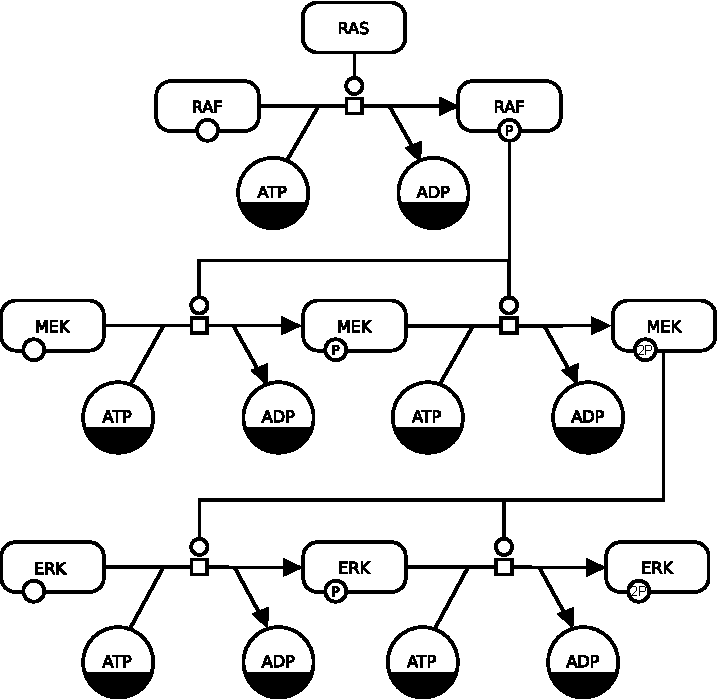
\includegraphics[scale=0.7]{examples/MAPK-only}
  \caption{This example of a \PD map uses two kinds of entity pool nodes: one
    for pools of different macromolecules (\sect{macromolecule}) and
    another for pools of simple chemicals (\sect{simpleChemical}).  Most
    \glyph{macromolecule} nodes in this map are adorned with \glyph{state
    variables} (\sect{stateVariable}) representing phosphorylation states.
    This map uses one type of \glyph{process node}, the \glyph{process} node
    (\sect{process}), and three kinds of connecting arc, \glyph{consumption} (\sect{consumption}), \glyph{production} (\sect{production}) and \glyph{catalysis}
    (\sect{catalysis}).  Finally, some entity pool nodes have dark bands
    along their bottoms; these are \glyph{clone markers} (\sect{cloneMarker}) indicating that the same
    pool nodes appear multiple times in the map.}
  \label{fig:eg1}
\end{figure}

The map in \fig{eg1} is a simple map for part of a mitogen-activated protein kinase (MAPK) cascade.  The larger nodes in the figure (some of which are in the shape of rounded rectangles and others in the shape of circles) represent biological materials---things like macromolecules and simple chemicals.  The biological materials are altered via processes, which are indicated in \PDl by lines with arrows and other decorations.  In this particular map, all of the processes happen to be the same: processes catalysed by biochemical entities.  The directions of the arrows indicate the direction of the processes; for example, unphosphorylated RAF kinase processes to phosphorylated RAF kinase via a process catalysed by RAS. Although ATP and ADP are shown as incidental to the phosphorylations on this particular graph, they are involved in the same process as the proteins getting phosphorylated. The small circles on the nodes for RAF and other entity pools represent state variables (in this case, phosphorylation sites). 

The essence of the \PDs is the \emph{change}: it shows how different entities in the system process from one form to another.  The entities themselves can be many different things.  In the example of \fig{eg1}, they are pools of either macromolecules or simple chemicals, but as will become clear later in this chapter, they can be other conceptual and material constructs as well.  Note also that we speak of \emph{entity pools} rather than individuals; this is because, in biochemical network models, one does not focus on single molecules, but rather collections of molecules of the same kind.  The molecules in a given pool are considered indistinguishable from each other.  The way in which one type of entity is transformed into another is conveyed by a \emph{process node} and links between entity pool nodes, and process nodes indicate influence by the entities on the processes.  In the case of \fig{eg1}, those links describe consumption \sect{consumption}, production \sect{production} and catalysis \sect{catalysis}, but others are possible.  Finally, nodes in \PDs are usually not repeated; if they do need to be repeated, they are marked with \emph{clone markers}---specific modifications to the appearance of the node (\sect{cloneMarker}). The details of this and other aspects of \PD notation are explained in the rest of this chapter.

\tab{component-summary} summarizes the different SBGN abstractions described in this chapter.

\newcolumntype{P}[1]{>{\raggedright\hspace{0pt}\arraybackslash}p{#1}}

\begin{table}[bh]
  \centering
  \small
  \begin{tabular}{@{}llP{2.4in}P{1.6in}@{}}
    \toprule
    \textbf{Component} & \textbf{Abbrev.} & \textbf{Role} & \textbf{Examples}\\
    \midrule
    Entity pool node
    & EPN
    & A population of entities that cannot be distinguished from each other
    & Specific macromolecules or other chemical species \\[0.5em]

    Container node	
    % 
    & CN
    & An encapsulation of one or more other SBGN constructs
    & Compartments \\[1.6em]

    Process node
    & PN
    & A process that transforms one or more EPNs into one or more other EPNs
    & Process, association, dissociation \\[0.5em]

    Arc
    & ---
    & Links between EPNs, CNs or Logical Operators to PNs or Logical operators
    & Production, catalysis, inhibition \\[0.5em]

    Logical operators
    & LO
    & Combines one or several inputs into one output
    & Boolean \emph{and}, \emph{or}, \emph{not} \\
    \bottomrule
  \end{tabular}
  \caption{Summary of \PD components and their roles.}
  \label{tab:component-summary}
\end{table}



%%% Local Variables: 
%%% mode: latex
%%% TeX-master: "../sbgn_PD-level1"
%%% End: 


\section{Controlled vocabularies used in \SBGNPDLone}\label{sec:CVs}

%%%%%%%%%%%%%%%%%%%%%%%%%%%%%%%%%%%%%%%%%%%%%%%%%%%%%%%%%%%%%%%%%%%%%%
%%%%                   Controlled vocabularies
%%%%%%%%%%%%%%%%%%%%%%%%%%%%%%%%%%%%%%%%%%%%%%%%%%%%%%%%%%%%%%%%%%%%%%
%\color{blue}

Some glyphs in SBGN \PDs can contain particular kinds of textual annotations conveying information relevant to the purpose of the glyph.  These annotations are \glyph{units of information} (\sect{unitInfo}) or \glyph{state variables}  (\sect{stateVariable}).  For example, multimers can have a unit of information conveying the number of monomers composing the multimer. 

Other cases are described throughout the rest of this chapter.

The text that appears as the unit of information decorating an Entity Pool Node (EPN) must in most cases be prefixed with a controlled vocabulary term indicating the type of information being expressed.  The prefixes are mandatory except in the case of macromolecule covalent modifications (\sect{covalent-mod-cv}).  
Without the use of controlled vocabulary prefixes, it would be necessary to have different glyphs to indicate different classes of information; this would lead to an explosion in the number of symbols needed.

In the rest of this section, we describe the controlled vocabularies (CVs) used in \SBGNPDLone.  
They cover the following categories of information: an EPN's material type, an EPN's conceptual type, covalent modifications on macromolecules, the physical characteristics of compartments, and cardinality (\eg of multimers).  
In each case, some CV terms are predefined by SBGN, but unless otherwise noted, \emph{they are not the only terms permitted}.  
Users may use other CV values not listed here.
In such cases, they should explain the term's meanings in a figure legend or other text accompanying the map.
% 
Users of CV values not listed here should \emph{strongly} attempt different prefixes from those listed in this document. 


\subsection{Entity pool node material types}
\label{sec:material-types-cv}

The material type of an EPN indicates its chemical structure and physical composition.  A list of common material types is shown in \tab{material-types-cv}, but others are possible.  The values are to be taken from the \sbo (\sbourl), specifically from the branch having identifier \sboid{SBO:0000240} (the \emph{material entity} under \emph{entity}).

\begin{table}[h]
  \centering
  \begin{tabular}{l>{\ttfamily}l>{\ttfamily}l}
    \toprule
    \textbf{Name}              & \textbf{\rmfamily Label} & \textbf{\rmfamily SBO term} \\
    \midrule
    Non-macromolecular ion     & mt:ion  & SBO:0000327\\
    Non-macromolecular radical & mt:rad  & SBO:0000328\\
    Ribonucleic acid           & mt:rna  & SBO:0000250\\
    Deoxyribonucleic acid       & mt:dna  & SBO:0000251\\
    Protein                    & mt:prot & SBO:0000297\\
    Polysaccharide             & mt:psac & SBO:0000249\\
    \bottomrule
  \end{tabular}
  \caption{A sample of values from the \emph{material types} controlled
    vocabulary (\sect{material-types-cv}).}
  \label{tab:material-types-cv}
\end{table}

The material types are in contrast to the \emph{conceptual types} (see below).  The distinction is that material types are about physical composition, while conceptual types are about roles.  For example, a strand of RNA is a material type, but its use as messenger RNA is a role.


\subsection{Entity pool node conceptual types}
\label{sec:conceptual-types-cv}

An EPN's \emph{conceptual type} indicates its function within the context of a given \PD.  A list of common conceptual types is shown in \tab{conceptual-types-cv}, but others are possible.  The values are to be taken from the \sbo (\sbourl), specifically from the branch having identifier \sboid{SBO:0000241} (the \emph{conceptual entity} under \emph{entity}).  

\begin{table}[h]
  \centering
  \begin{tabular}{l>{\ttfamily}l>{\ttfamily}l}
    \toprule
    \textbf{Name}              & \textbf{\rmfamily Label} & \textbf{\rmfamily SBO term} \\
    \midrule
    Gene                      & ct:gene   & SBO:0000243\\
    Transcription start site  & ct:tss    & SBO:0000329\\
    Gene coding region        & ct:coding & SBO:0000335\\
    Gene regulatory region    & ct:grr    & SBO:0000369\\
    Messenger RNA             & ct:mRNA   & SBO:0000278\\
    \bottomrule
  \end{tabular}
  \caption{A sample of values from the \emph{conceptual types} vocabulary
    (\sect{conceptual-types-cv}).}
  \label{tab:conceptual-types-cv}
\end{table}


\subsection{Macromolecule covalent modifications}
\label{sec:covalent-mod-cv}

A common reason for the introduction of state variables (\sect{stateVariable}) on an entity is to allow access to the configuration of possible covalent modification sites on that entity.  For instance, a macromolecule may have one or more sites where a phosphate group may be attached; this change in the site's configuration (\ie being either phosphorylated or not) may factor into whether, and how, the entity can participate in different processes.  Being able to describe such modifications consistently is the motivation for the existence of SBGN's covalent modifications controlled vocabulary.

Table~\ref{tab:covalent-mod-cv} lists selected common types of covalent modifications.
The most common values are defined by the \sbo in the branch having identifier \sboid{SBO:0000210} (\emph{addition of a chemical group} under \emph{interaction}$\rightarrow$\emph{process}$\rightarrow$\emph{biochemical or transport reaction}$\rightarrow$\emph{biochemical reaction}$\rightarrow$\emph{conversion}).  The labels shown in \tab{covalent-mod-cv} are defined by \SBGNPDLone; for all other kinds of modifications not listed here, the author of a \PD must create a new label (and should also describe the meaning of the label in a legend or text accompanying the map).

\begin{table}[h]
  \centering
  \begin{tabular}{l>{\ttfamily}l>{\ttfamily}l}
    \toprule
    \textbf{Name}   & \textbf{\rmfamily Label} & \textbf{\rmfamily SBO term} \\
    \midrule
    Acetylation     & Ac    & SBO:0000215\\
    Glycosylation   & G     & SBO:0000217\\
    Hydroxylation   & OH    & SBO:0000233\\
    Methylation     & Me    & SBO:0000214\\
    Myristoylation  & My    & SBO:0000219\\
    Palmytoylation  & Pa    & SBO:0000218\\
    Phosphorylation & P     & SBO:0000216\\
    Prenylation     & Pr    & SBO:0000221\\
    Protonation     & H     & SBO:0000212\\
    Sulfation       & S     & SBO:0000220\\
    Ubiquitination  & Ub    & SBO:0000224\\
    \bottomrule
  \end{tabular}
  \caption{A sample of values from the \emph{covalent modifications} vocabulary
    (\sect{covalent-mod-cv}).}
  \label{tab:covalent-mod-cv}
\end{table}


\subsection{Physical characteristics}
\label{sec:physical-characteristics-cv}

\SBGNPDLone defines a specific unit of information for describing particular common physical characteristics.  
\tab{physical-characteristics-cv} lists the particular values defined by \SBGNPDLone.  %
%The values correspond to the \sbo branch with identifier \sboid{SBO:0000255} (\emph{physical characteristic} under \emph{quantitative parameter}).
It is anticipated that these will be used to describe the nature of a \glyph{perturbing agent} (section \ref{sec:perturbing agent}) or a \glyph{phenotype} (section \ref{sec:phenotype}).

\begin{table}[h]
  \centering
  \begin{tabular}{l>{\ttfamily}l>{\ttfamily}l}
    \toprule
    \textbf{Name}   & \textbf{\rmfamily Label} & \textbf{\rmfamily SBO term} \\
    \midrule
    Temperature   & pc:T  & SBO:0000147\\
    Voltage       & pc:V  & SBO:0000259\\
    pH            & pc:pH & SBO:0000304\\
    \bottomrule
  \end{tabular}
  \caption{A sample of values from the \emph{physical
      characteristics} vocabulary (\sect{physical-characteristics-cv}).}
  \label{tab:physical-characteristics-cv}
\end{table}


\subsection{Cardinality}
\label{sec:cardinality-cv}

\SBGNPDLone defines a specific unit of information usable on multimers for describing the number of monomers composing the multimer.  \tab{cardinality-cv} shows the way in which the values must be written.  Note that the value is a positive non-zero integer, and not (for example) a range.  There is no provision in \SBGNPDLone for specifying a range in this context because it leads to problems of entity identifiability.

\begin{table}[h]
  \centering
  \begin{tabular}{l>{\ttfamily}l>{\ttfamily}l}
    \toprule
    \textbf{Name}   & \textbf{\rmfamily Label} & \textbf{\rmfamily SBO term} \\
    \midrule
    cardinality    & N:\#  & SBO:0000364\\
    \bottomrule
  \end{tabular}
  \caption{The format of the possible values for the
    \emph{cardinality} unit of information
    (\sect{cardinality-cv}).  Here, \texttt{\#} stands for the
    number; for example, ``\texttt{N:5}''.}
  \label{tab:cardinality-cv}
\end{table}



% \normalcolor


% The following is for [X]Emacs users.  Please leave in place.
% Local Variables:
% TeX-master: "../sbgn_PD-level1"
% End:


\section{Auxiliary Units}

Auxiliary units are glyphs that decorate other glyphs, providing additional information that may be useful to the reader. These can provide annotation (\glyph{unit of information}), state information (\glyph{state variable}) or indicate duplication of entity pool nodes (\glyph{clone marker}).

\subsection{Glyph: \glyph{Unit of information}}
\label{sec:unitInfo}

When representing biological entities, it is often necessary to convey some abstract information about the entity's function that is not related to its role in the map.  The \glyph{unit of information} is a decoration that can be used in this situation to add information to an EPN.  Some example uses include: characterizing a logical part of an entity such as a functional domain (a binding domain, a catalytic site, a promoter, etc.), or the information encoded in the entity (an exon, an open reading frame, etc.).  A \glyph{unit of information} can also convey information about the physical environment, or the specific type of biological entity it is decorating. A \glyph{unit of information} is represented by a rectangle overlapping the border of the \glyph{EPN} being annotated.

The label carried by \glyph{unit of information} defines the information it carries.  For certain predefined types of information having controlled vocabularies associated with them, SBGN defines specific prefixes that must be included in the label to indicate the type of information in question.  The controlled vocabularies predefined in \SBGNPDLone are described in \sect{CVs}.

\begin{figure}[H]
  \centering
  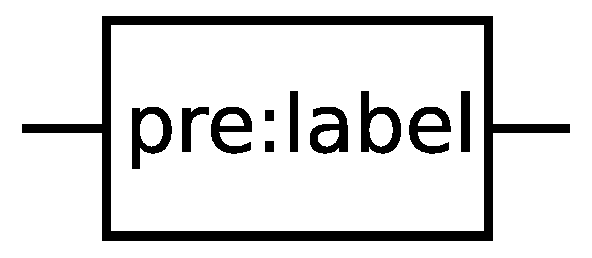
\includegraphics[scale = 0.3]{images/unitInformation}
  \caption{The \PD glyph for \glyph{unit of information}.}
  \label{fig:unitInfo}
\end{figure}




% The following is for [X]Emacs users.   Please leave in place.
% Local Variables:
% TeX-master: "../sbgn_PD-level1"
% End:



% $HeadURL$

\subsection{Glyph: \glyph{State variable}}
\label{sec:stateVariable}

Many biological entities such as molecules can exist in different states, meaning different physical or informational configurations.
These states can arise for a variety of reasons.
For example, macromolecules can be subject to post-synthesis modifications, wherein residues of the macromolecules (amino acids, nucleosides, or glucid residues) are modified through covalent linkage to other chemicals.
Other examples of states are alternative conformations as in the closed/open/desensitised conformations of a transmembrane channel, and the active/inactive forms of an enzyme.


To describe such states, the \PD introduces the concept of the state variable.
A state variable of a biological entity usually has a name (\eg ``S122'' to indicate residue Serine 122 of a protein), and can be assigned a value (\eg ``P'', to indicate a phosphate group).
Such a state variable models a dimension along which the state of the overall entity can vary.
The state of an entity can then be described by the current values assigned to all its state variables, and of all its possible components, recursively.
A state variable may be assigned no value; an example of a situation where this might arise is an unphosphorylated phosphorylation site.
% 
A state variable might also be unnamed, in cases where there is no ambiguity between this state variable and another state variable carried by the same entity (\eg when an entity carries a unique state variable, it might be unnamed).
% 
In \PD, state variables, together with the values assigned to them, are represented using the \glyph{state variable} glyph.


\begin{glyphDescription}

\glyphSboTerm
Not applicable.


\glyphIncoming
None.



\glyphOutgoing
None.


\glyphContainer
A \glyph{state variable} is represented by a ``stadium'' shape, that is two semicircles of the same radius joined by parallel segments, as shown in \novreffig{state-var}.

The centre of the shape should be placed on the border of the EPN.

% 
In previous versions of this specification, the \glyph{state variable} was represented by an elliptic shape.
This symbol is now \textbf{deprecated} in favour of the stadium shape described above.

% 



\glyphLabel
A \glyph{state variable} is identified by a label that is  a string of characters.
The characters cannot be distributed on several lines.
The centre of the label must be placed on the centre of the container.
The label may extend outside of the container.
The label is constituted of two substrings separated by the character ``@'', the first one indentifying the value of the state variable, and the second one its name.
The character ``@'' is omitted when the state variable is unnamed.
Aternatively, the substring identifying the name of the state variable may be displayed using a second label, placed outside of the shape.
This is, however, strongly discouraged.


% \glyphLabel
% A \glyph{state variable} is identified by a label that is an unbordered box containing a string of characters.
% The characters cannot be distributed on several lines.
% The centre of the label must be placed on the centre of the shape.
% The label may extend outside of the shape.
% The label is constituted of one or two substrings.
% The first substring, that is mandatory, identifies the value of the \glyph{state variable}.
% It may be empty; an example of a situation where this might arise is an unphosphorylated phosphorylation site.
% The second substring, which is optional, identifies the variable of the \glyph{state variable}, preceded by the character ``@''.
% This substring should be included in the label if confusion is possible between several \glyph{state variables} (\eg several phosphorylation sites).
% In previous versions of this specification, the substring identifying the variable could be displayed in an additional label lying outside of the \glyph{state variable}'s shape.
% This is now \textbf{deprecated}.

\glyphAux
None.

\end{glyphDescription}

\begin{figure}[H]
  \centering
  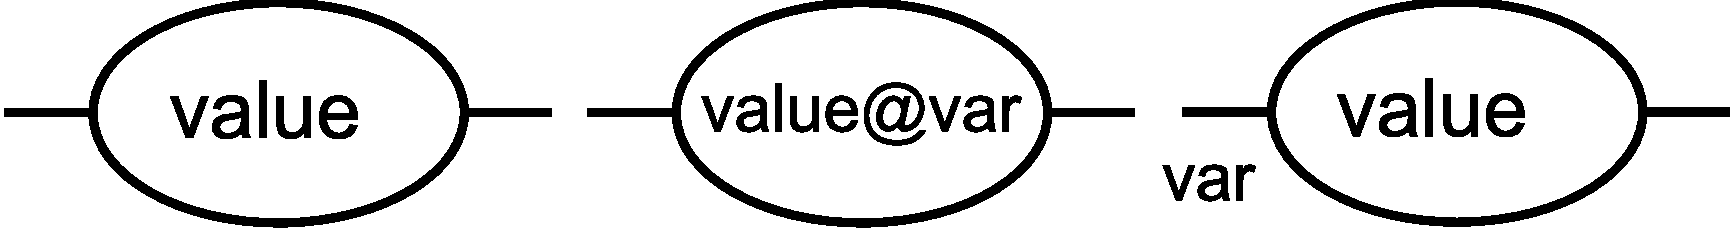
\includegraphics{images/stateVariable}
  \caption{The \PD glyph for \glyph{state variable}, shown with a value and a variable on the far left, with only a value on the middle-left, with an additional label for the variable on the middle-right (discouraged), and decorating a \glyph{macromolecule} (\sect{macromolecule}) on the far right.}
  \label{fig:state-var}
\end{figure}

\begin{figure}[H]
  \centering
    \begin{tabular}{lc}
        A & \raisebox{-\height}{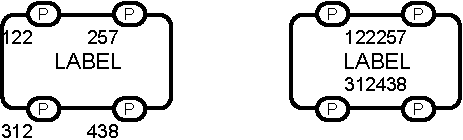
\includegraphics{examples/wrongStateVariablesA}}\\
        B & \raisebox{-\height}{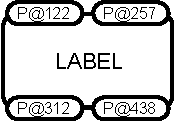
\includegraphics{examples/wrongStateVariablesB}}
    \end{tabular}
  \caption{A. Examples of discouraged use of \glyph{state variables}. B. Encouraged use.}
 \label{fig:wrong-state-var}
\end{figure}

% The following is for [X]Emacs users.  Please leave in place.
% Local Variables:
% TeX-master: "../sbgn_PD-level1"
% End:



\subsection{Glyph: \glyph{Clone marker}}
\label{sec:cloneMarker}

It is sometimes necessary to represent the same \glyph{EPN} several times. Otherwise, the resulting graph is so tightly connected that the map becomes unreadable. An example would be the representation of currency molecules such as ATP. However, we must indicate the fact, so that a reader knows the processes involving this particular glyph are not the only processes involving the \glyph{EPN}. If an \glyph{EPN} is duplicated on a map, we therefore mark all its graphical reprensation with a \glyph{clone marker} auxiliary unit.  This marker provides the reader with a visual indication that this node has been cloned, and that at least one other occurrence of the \glyph{EPN} can be found in the map (or in a submap; see \sect{submap}).  The clone marker takes two forms, simple and labeled, depending on whether the node being cloned can carry state variables. Note that an \glyph{EPN} belongs to a single compartment. If two glyphs labelled ``X'' are located in two different compartments, such as ATP in cytosol and ATP in mitochondrial lumen, they represent different \glyph{EPNs}, and therefore do not need to be marked as cloned (and if they are, they are not part of the same clone).

The simple (unlabeled) \glyph{clone marker} is a portion of the surface of an \glyph{EPN} that has been modified visually through the use of a different shade, texture, or color.  \fig{simpleCloneMarker} illustrates this. The \glyph{clone marker} occupies the lower part of the \glyph{EPN}. The filled area must be smaller than the unfilled one.

\begin{figure}[H]
  \centering
  
\includegraphics[scale = 0.3]{images/simpleCloneMarker}
  \caption{The \PD glyph for \glyph{simple clone marker} applied to a \glyph{simple chemical}}
  \label{fig:simpleCloneMarker}
\end{figure}

Unlike the \glyph{simple clone marker}, the \glyph{labeled clone marker} includes (unsurprisingly, given its name) an identifying label that can be used to identify equivalent clones elsewhere in the map.  This is particularly useful for stateful \glyph{EPNs}, because these can have a large number of state variables displayed and therefore may be difficult to visually identify as being identical. The filled area must be smaller than the unfilled one, but the be large enough to have a height larger than the \glyph{clone marker}'s label (cf below).

\begin{figure}[H]
  \centering
  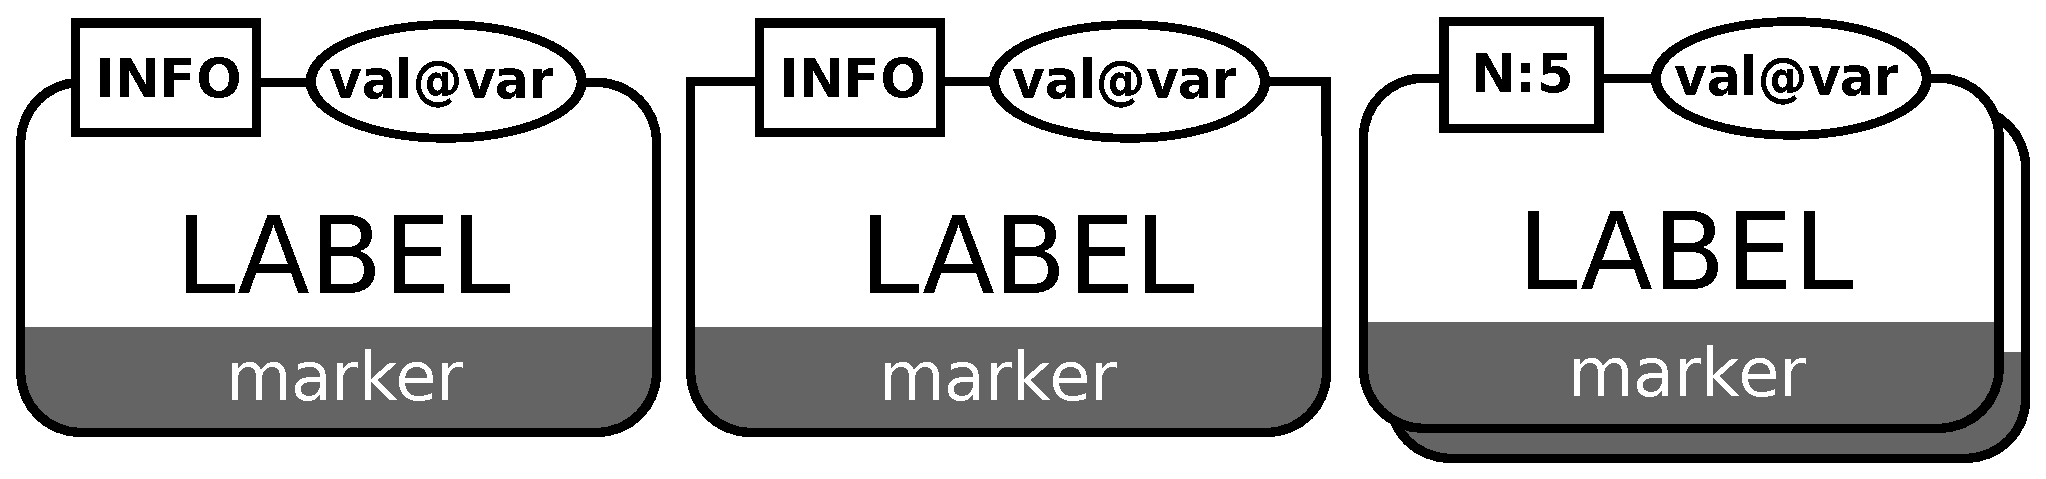
\includegraphics[scale = 0.3]{images/labeledCloneMarker}
  \caption{The \PD glyph for \glyph{labeled clone marker} applied to a \glyph{multimer} of  \glyph{macromolecules}.}
  \label{fig:labeledCloneMarker}
\end{figure}



%%%%%%%%%%%%%%%%%%%%%%%%%%%%%%%%%%%%%%%%%%%%%%%%%%%%%%%%%%%%%%%%%%%%%%
%%%%%%%%%%%%%%%%%%%%%%%%%%%%%%%%%%%%%%%%%%%%%%%%%%%%%%%%%%%%%%%%%%%%%%
%%%%                   State nodes
%%%%%%%%%%%%%%%%%%%%%%%%%%%%%%%%%%%%%%%%%%%%%%%%%%%%%%%%%%%%%%%%%%%%%%
%%%%%%%%%%%%%%%%%%%%%%%%%%%%%%%%%%%%%%%%%%%%%%%%%%%%%%%%%%%%%%%%%%%%%%

\section{Entity pool nodes}\label{sec:EPNs}

An entity pool is a population of entities that cannot be distinguished from each other, when it comes to the \SBGNPDLone map. For instance all the molecular  entities that fulfill the same role in a given process form an entity pool. As a result, an entity pool can represent different granularity levels, such as all the proteins, all the instances of a given protein, only certain forms of a given protein. To belong to a different compartment is sufficient to belong to different entity pools. Calcium ions in the endoplasmic reticulum and calcium ions in the cytosol belong to different entity pools when it comes to representing calcium release from the endoplasmic reticulum.

The \PD contains six glyphs representing classes of material entities: \glyph{unspecified entity} (\sect{unspecifiedEntity}), \glyph{simple chemical} (\sect{simpleChemical}), \glyph{macromolecule} (\sect{macromolecule}), \glyph{nucleic acid feature} (\sect{genetic}), \glyph{multimer} (\sect{multimer}) and \glyph{complex} (\sect{complex}).  (Specific types of macromolecules, such as protein, RNA, DNA, polysaccharide, and specific simple chemicals are not defined by \PD but may be part of future levels of SBGN.)  In addition to the material entities, \PD represents three conceptual entities: \glyph{source}, \glyph{sink} (\sect{sourceSink}), and \glyph{perturbing agent} (\sect{perturbing agent}).  Material and conceptual entities can optionally carry auxiliary units such as \glyph{units of information} (\sect{unitInfo}), \glyph{state variables}  (\sect{stateVariable}) and \glyph{clone markers} (\sect{cloneMarker}).

% $HeadURL$

\subsection{Glyph: \glyph{Unspecified entity}}
\label{sec:unspecifiedEntity}

The simplest type of EPN is the \glyph{unspecified entity}: one whose type is unknown or simply not relevant to the purposes of the map.
This arises, for example, when the existence of the entity has been inferred indirectly, or when the entity is merely a construct introduced for the needs of a map, without direct biological relevance.
These are examples of situations where the \emph{unspecified entity} glyph is appropriate.
(Conversely, for cases where the identity of the entities composing the pool is known, there exist other, more specific glyphs described elsewhere in the specification.)

\begin{glyphDescription}

\glyphSboTerm
 SBO:0000285 ! material entity of unspecified nature


\glyphIncoming
Zero or more \glyph{production} arcs (\sect{production}).



\glyphOutgoing
Zero or more \glyph{consumption} arcs (\sect{consumption}), \glyph{modulation arcs} (\sect{modulations}), \glyph{logic arcs} (\sect{logicArc}), or \glyph{equivalence arcs} (\sect{equivalenceArc}).


\glyphContainer
A \glyph{unspecified entity} is represented by an elliptic shape, as shown in \fig{unspecified}.
Note that the shape must remain an ellipse to avoid confusion with \glyph{simple chemical}, which is represented with a stadium shape (\sect{simpleChemical}).

\glyphLabel
A \glyph{unspecified entity} is identified by a label  that is a string of characters that may be distributed on several lines to improve readability.
The centre of the label must be placed on the centre of the container.
The label may extend outside of the container.



\glyphAux
An \glyph{unspecified entity} can carry a \glyph{clone marker} (see \sect{cloneMarker}).

\end{glyphDescription}

\begin{figure}[H]
  \centering
  
\includegraphics{images/build/unspecified.pdf}
  \caption{The \PD glyph for \glyph{unspecified entity}.}
  \label{fig:unspecified}
\end{figure}

% The following is for [X]Emacs users.   Please leave in place.
% Local Variables:
% TeX-master: "../sbgn_PD-level1"
% End:


\subsection{Glyph: \glyph{Simple chemical}}
\label{sec:simpleChemical}

In SBGN \PDs, a simple chemical is defined as the opposite of a macromolecule (\sect{macromolecule}): it is a chemical compound that is \emph{not} formed by the covalent linking of pseudo-identical residues.  Examples of simple chemicals are an atom, a monoatomic ion, a salt, a radical, a solid metal, a crystal, etc. A \glyph{simple chemical} is represented by a circular
container, as depicted in \fig{simpleChemical}. To avoid confusion with the Unspecified Entity (\ref{sec:unspecifiedEntity}), this glyph must remain a circle and cannot be deformed into an ellipse.

\begin{figure}[H]
  \centering
  \includegraphics[scale = 0.3]{images/simpleChemical}
  \caption{The \PD glyph for \glyph{simple chemical}.}
  \label{fig:simpleChemical}
\end{figure}

Examples of \glyph{simple chemicals} are presented in \fig{simpleChemical-examples}.

\begin{figure}[H]
  \centering
  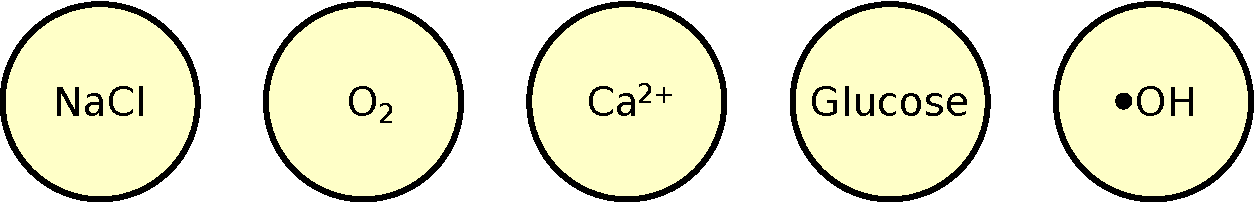
\includegraphics[scale = 0.5]{images/simpleChemical-examples}
  \caption{Examples of \glyph{simple chemicals}. From left to right: sodium chloride (a salt), dioxygene (a elemental molecule), calcium ion, glucose (an heteroatomics molecule), hydroxyl radical.}
  \label{fig:simpleChemical-examples}
\end{figure}

% $HeadURL: https://sbgn.svn.sourceforge.net/svnroot/sbgn/ProcessDiagram/tags/L1V1.3Full/sources/macromolecule.tex $

\subsection{Glyph: \glyph{Macromolecule}}
\label{sec:macromolecule}

Many biological processes involve \emph{macromolecules}: biochemical substances that are built up from the covalent linking of pseudo-identical units.  Examples of macromolecules include proteins, nucleic acids (RNA, DNA), and polysaccharides (glycogen, cellulose, starch, etc.).  Attempting to define a separate glyph for all of these different molecules would lead to an explosion of symbols in SBGN, so instead, \SBGNPDLone defines only one glyph for all macromolecules.  The same glyph is to be used for a protein, a nucleic acid, a complex sugar, and so on.  The exact nature of a particular macromolecule in a map is then clarified using its label and decorations, as will become clear below.  A \glyph{macromolecule} is represented by a rectangular container with rounded corners, as illustrated in \fig{macromolecule}. 

\begin{figure}[H]
  \centering
  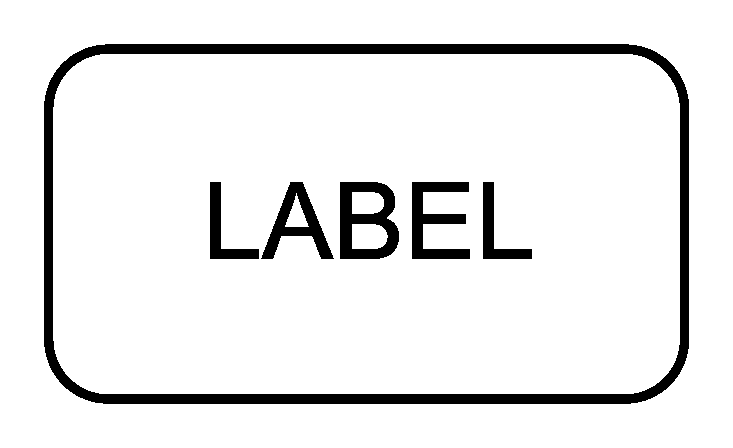
\includegraphics[width = 1.25in]{images/macromolecule-plain}
  \caption{The \PD glyph for \glyph{macromolecule}.}
  \label{fig:macromolecule}
\end{figure}

Examples of \glyph{macromolecules} are presented in \fig{macromolecule-examples}.

\begin{figure}[H]
  \centering
  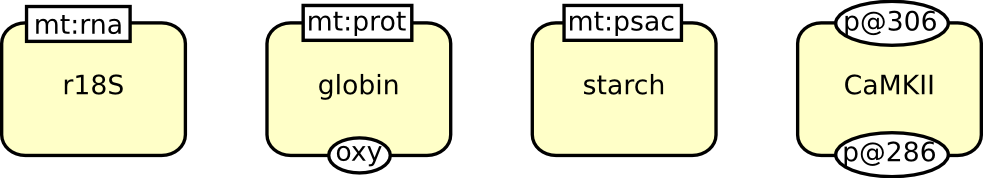
\includegraphics[scale = 0.5]{images/macromolecule-examples}
  \caption{Examples of \glyph{macromolecules}. From left to right: the macromolecule of 18S ribosomal RNA, globin (a protein) in the oxygenated state, a molecule of starch (polymer of glucose), calcium calmodulin kinase 2 phosphorylated on threonine 286 and 306.}
  \label{fig:macromolecule-examples}
\end{figure}




% The following is for [X]Emacs users.   Please leave in place.
% Local Variables:
% TeX-master: "../sbgn_PD-level1"
% End:

% $HeadURL$

\subsection{Glyph: \glyph{Nucleic acid feature}}
\label{sec:genetic}

The \emph{Nucleic acid feature} construct in SBGN is meant to represent a fragment of a macromolecule carrying genetic information.  A common use for this construct is to represent a gene or transcript.  The label of this EPN and its \emph{units of information} are often important for making the purpose clear to the reader of a map.

\begin{glyphDescription}

\glyphSboTerm SBO:0000354 !  informational molecule segment

\glyphContainer A \glyph{nucleic acid feature} is represented by a rectangular container whose bottom half has rounded corners, as shown in \fig{genetic}. This design reminds that we are fundamentally dealing with a unit of information, but this information is carried by a macromolecule.

\glyphLabel The identity of a particular \glyph{Nucleic acid feature} is established by a label placed in an unordered box containing a string of characters.  The characters may be distributed on several lines to improve readability, although this is not mandatory.  The label box must be attached to the center of the container.  The label may spill outside of the container.

\glyphAux A \glyph{nucleic acid feature} can carry state variables (\sect{stateVariable}) that add information about its precise state.  The state of a \glyph{nucleic acid feature} is therefore defined as the vector of all its state variables. 

A \glyph{nucleic acid feature} can also carry one or several \glyph{units of information} (\sect{unitInfo}).  These can characterize a \glyph{nucleic acid feature}'s domain, such as a binding site, or an exon.  Particular \glyph{units of information} carry the material type (\sect{material-types-cv}) and the conceptual type (\sect{conceptual-types-cv}) of the \glyph{nucleic acid feature}. 

A \glyph{nucleic acid feature} may also carry a \glyph{clone marker}
(\sect{cloneMarker}).

\end{glyphDescription}


\begin{figure}[H]
  \centering
  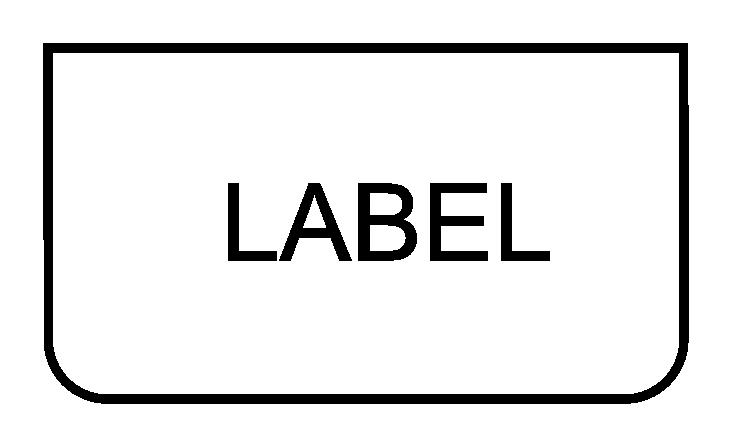
\includegraphics[width = 1.25in]{images/genetic-plain} \hspace*{2em}
  \raisebox{0.04in}{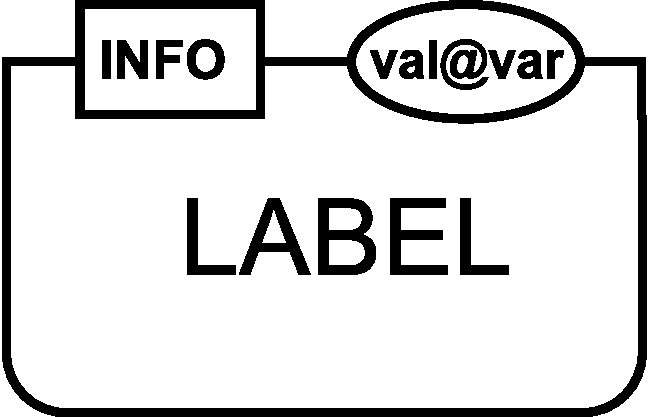
\includegraphics[width = 1.25in]{images/genetic}}
  \caption{The \PD glyph for \glyph{nucleic acid feature}, shown plain and
    unadorned on the left and with an additional state variable and a
    unit of information on the right.} 
  \label{fig:genetic}
\end{figure}

% The following is for [X]Emacs users.  Please leave in place.
% Local Variables:
% TeX-master: "../sbgn_PD-level1"
% End:

\subsection{Glyph: \glyph{Multimer}}
\label{sec:multimer}

As its name implies, a multimer is an aggregation of multiple identical or pseudo-identical entities held together by non-covalent bonds (thus, they are distinguished from polymers by the fact that the later involve covalent bonds).
Here,  \emph{pseudo-identical} refers to the possibility that the entities differ chemically but retain some common global characteristic, such as a structure or function, and so can be considered identical within the context of the SBGN \PD.
An example of this is the homologous subunits in a hetero-oligomeric receptor.

SBGN \PD defines four different \glyph{multimer} glyphs: \glyph{simple chemical multimer}, \glyph{macromolecule multimer}, \glyph{nucleic acid feature multimer} and \glyph{complex multimer}.



\begin{glyphDescription}

\glyphSboTerm
\begin{tabular}{l l}
    & SBO:0000286 ! multimer\\
\glyph{Simple chemical multimer} & SBO:0000421 ! multimer of simple chemicals\\
\glyph{Macromolecule multimer} & SBO:0000420 ! multimer of macromolecules \\
\glyph{Complex multimer} & SBO:0000418 ! multimer of complexes \\
\glyph{Nucleic acid feature multimer} & SBO:0000419 ! multimer of informational molecule segments \\
\end{tabular}


\glyphIncoming
Zero or more \glyph{production} arcs (\sect{production}).



\glyphOutgoing
Zero or more \glyph{consumption} arcs (\sect{consumption}), \glyph{modulation arcs} (\sect{modulations}), \glyph{logic arcs} (\sect{logicArc}), or \glyph{equivalence arcs} (\sect{equivalenceArc}).



\glyphContainer
Each \glyph{multimer} is represented by a different shape depending on the bio-molecular nature of its pseudo-identical subunits, as shown in \tab{multimer_containers}.
The shape of a \glyph{multimer} consists of two \glyph{subunits} or \glyph{EPNs} shapes shifted horizontally and vertically, and stacked on top of another.




\glyphLabel
A \glyph{subunit} is identified by a label that is   a string of characters that may be distributed on several lines to improve readability.
% 
The centre of the label must be placed on the centre of the shape.
The label may extend outside of the shape.
The label should refer to the pseudo-identical subunits, and not to the multimer itself.



\glyphAux A \glyph{multimer} may carry auxiliary units, depending on its type.

A \glyph{macromolecule}, \glyph{nucleic acid feature}, or \glyph{complex multimer} can carry one or more \glyph{state variables} that add information about its state (\sect{stateVariable}).
The state of such a \glyph{multimer} is defined as the set of all its \glyph{state variables}.

A \glyph{multimer} of any type can carry one or more \glyph{units of information} (\sect{unitInfo}).
These can characterize a domain, such as a binding site.
Particular \glyph{units of information} are available for describing the material type (\sect{material-types-cv}), conceptual type (\sect{conceptual-types-cv}) and the cardinality (\sect{cardinality-cv}) of such a \glyph{multimer}.

Note that a \glyph{state variable} or a \glyph{unit of information} carried by a \glyph{multimer} actually applies to each of the subunits individually.
If instead the \glyph{state variables} or the \glyph{units of information} are meant to apply to the whole multimeric assembly, a \glyph{macromolecule} (\sect{macromolecule}) or a \glyph{complex} (\sect{complex}) should be used instead of a \glyph{multimer}.
An assembly containing some \glyph{state variables} or \glyph{units of information} applicable to the subunits, and other \glyph{state variables} or \glyph{units of information} applicable to the assembly (for instance opening of a channel and phosphorylation of each of its subunits) should be represented by a \glyph{complex} (\sect{complex}).

Finally, a \glyph{simple chemical multimer} can also carry a \glyph{simple clone marker} (\sect{cloneMarker}), and a \glyph{macromolecule}, \glyph{nucleic acid feature} or \glyph{complex multimer} a \glyph{labelled clone marker} (\sect{cloneMarker}).

\end{glyphDescription}

\begin{table}[h]
\begin{tabu}{X[c,m]X[c,m]X[c,m]X[c,m]}
    \toprule
    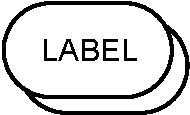
\includegraphics[valign = m]{images/simple_chemical-multimer} & 
\includegraphics[valign = m]{images/macromolecule-multimer} & 
\includegraphics[valign = m]{images/genetic-multimer} & 
\includegraphics[valign = m]{images/complex-multimer}\\[0.5cm]
    \glyph{simple chemical multimer} & \glyph{macromolecule multimer} & \glyph{nucleic acid feature multimer} & \glyph{complex multimer}\\
	\bottomrule
\end{tabu}
\caption{The \PD glyphs for the different types of \glyph{multimers}.}
\label{tab:multimer_containers}
\end{table}

% \begin{figure}[H]
%   \centering
%   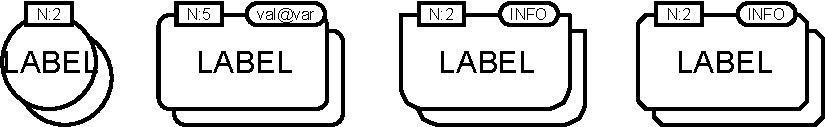
\includegraphics[scale = 0.3]{images/multimer}
%   \caption{The \PD glyph for \glyph{multimer} with an additional unit of information containing the cardinality.}
%   \label{fig:multimer}
% \end{figure}
% 

% The following is for [X]Emacs users.  Please leave in place.
% Local Variables:
% TeX-master: "../sbgn_PD-level1"
% End:

% $HeadURL$

%%%%%%%%%%%%%%%%%%%%%%%%%%%%%%%%%%%%%%%%%%%%%%%%%%%%%%%%%%%%%%%%%%%%%%
%%%%                   Complex
%%%%%%%%%%%%%%%%%%%%%%%%%%%%%%%%%%%%%%%%%%%%%%%%%%%%%%%%%%%%%%%%%%%%%%

\subsection{Glyph: \glyph{Complex}}\label{sec:complex}

A \glyph{complex} represents a pool of biochemical entities, each composed of other biochemical entities, whether macromolecules, simple chemicals, multimers, or other complexes. The resulting entity may have its own identity, properties and function in an SBGN map.
The \glyph{complex} can be described by the set of \glyph{subunits} \add{(\sect{subunit})} it contains (see \fig{complexSubunits}). This description is entirely optional and is there to assist the user with a visual shorthand about the composition of the complex.
% \rougny{Chaneg first sentence to ``A complex represents a pool if biochemical entities, each composed of other biochemical entities...''?}

\begin{glyphDescription}

\glyphSboTerm
SBO:0000253 ! non-covalent complex

\add{
\glyphIncoming
Zero or more \glyph{production} arcs (\sect{production}).
}

\add{
\glyphOutgoing
Zero or more \glyph{consumption} arcs (\sect{consumption}), \glyph{modulation arcs} (\sect{modulations}), \glyph{logic arcs} (\sect{logicArc}), or \glyph{equivalence arcs} (\sect{equivalenceArc}).
}

\glyphContainer
\corr{A \glyph{complex} possesses its own container box surrounding the juxtaposed container boxes of its components.
This container box is a rectangle with cut-corners (an octagonal box with sides of two different lengths). The size of the cut-corners are adjusted so that there is no overlap between the container and the components. The container boxes of the components must not overlap.}{
A \glyph{complex} is represented by a rectangular shape with cut-corners (that is, an octogonal shape with sides of two different lengths).
If the \glyph{complex} is described by a set of \glyph{subunits}, then its shape should surround those of its \glyph{subunits}, and the size of the cut-corners should be adjusted so that there is no overlap between its shape and those of its \glyph{subunits}.
The shapes of the \glyph{subunits} must not overlap.}

\glyphLabel
A \glyph{complex} is identified by a label that is \corr{an unbordered box containing}{} a string of characters \corr{.
The characters}{that} may be distributed on several lines to improve readability\corr{, although this is not mandatory}.
\corr{Ideally, the label box should be attached to the midway between the border of the complex's container box and the border of the components' container boxes. However, if the \glyph{complex} contains \glyph{subunits} glyphs then the label may be positioned to optimise the clarity and avoid overlapping.}{
In the case where the \glyph{complex} is not described by a set of \glyph{subunits}, the centre of the label must be placed on the centre of the \glyph{complex}'s shape.
In the case where the \glyph{complex} is described by a set of \glyph{subunits}, the label may be positioned to optimize the clarity and avoid overlapping, ideally between the bottom-most or the upper-most \glyph{subunit} and the border of the \glyph{complex}.
}

\glyphAux
A \glyph{complex} can carry one or more \glyph{state variables} that add information about its state (\sect{stateVariable}).
\corr{The state of a \glyph{complex} is defined as the set of all its \glyph{state variables}}{} \corr{and all the state variables of all its components}{}.\rougny{In old v2, the state of a complex is only defined by its state variables, not additionally by those of its subunits} \blinov{Talking about the state of a complex is confusing.}

A \glyph{complex} can also carry one or more \glyph{units of information} (\sect{unitInfo}).
These can characterise a domain, such as a binding site.
Particular \glyph{units of information} are available for describing the material type (\sect{material-types-cv}) and the conceptual type (\sect{conceptual-types-cv}) of a \glyph{complex}.

Finally, a \glyph{complex} can also carry a \glyph{labelled clone marker} (see \sect{cloneMarker}).

\end{glyphDescription}

\begin{figure}[H]
  \centering
  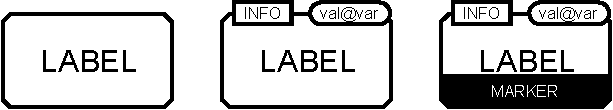
\includegraphics{images/complex-combined}
  \caption{The \PD glyph for \glyph{complex}, shown plain and unadorned on the left, with an additional \glyph{state variable} and a \glyph{unit of information} in the middle, and with a \glyph{labelled clone marker} on the right.}
  \label{fig:complex}
\end{figure}

% The following is for [X]Emacs users.  Please leave in place.
% Local Variables:
% TeX-master: "../sbgn_PD-level1"
% End:


% $HeadURL$

\subsection{Glyph: \glyph{Source} and \glyph{Sink}}
\label{sec:sourceSink}

It is useful to have the ability to represent the creation of an entity or
a state from an unspecified source, that is, from something that one does
not need or wish to make precise.  For instance, in a model where the
production of a protein is represented, it may not be desirable to
represent all of the amino acids, sugars and other metabolites used, or the
energy involved in the protein's creation.  Similarly, we may not wish to
bother representing the details of the destruction or decomposition of some
biochemical species into a large number of more primitive entities,
preferring instead to simply say that the species ``disappears into a
sink''.  Yet another example is that one may need to represent an input
(respectively, output) into (resp. from) a compartment without explicitly
representing a transport process from a source (resp. to a target).

For these and other situations, SBGN defines two glyphs that use the same symbol for explicitly
representing the involvement of an unspecified source or sink.  The symbol
used in SBGN is borrowed from the mathematical symbol for ``empty set'',
but it is important to note that it does not actually represent a true
absence of everything or a physical void---it represents the absence of the
corresponding structures in the model, that is, the fact that these sources
or sinks are conceptually outside the scope of the map. The reason that we
regard the \glyph{Source} and \glyph{Sink} as different glyphs is that they have different
syntax and semantics (the former only connects to a \glyph{Consumption} arc and the latter
a \glyph{Production} arc). This is mainly an issue for software tools and those mapping to
and from SBGN from other notations of exchange formats.

A frequently asked question is, why bother having an explicit symbol at
all?  The reason is that one cannot simply use an arc that does not
terminate on a node, because the dangling end could be mistaken to be
pointing to another node in the map.  This is specially true if the
map is rescaled, causing the spacing of elements in the map to
change.  The availability and use of an explicit symbol for sources and
sinks is critical.

\begin{glyphDescription}

\glyphSboTerm SBO:0000291 ! empty set

\glyphContainer A \glyph{source} or \glyph{sink} is represented by the mathematical symbol for ``empty
set'', that is, a circle crossed by a bar linking the upper-right and
lower-left corners of an invisible square drawn around the circle ($\emptyset$).
\fig{sourceSink} illustrates this.  The symbol should be linked to one
and only one edge in a map.

\glyphLabel A \glyph{source} or \glyph{sink} does not carry any labels.

\glyphAux A \glyph{source} or \glyph{sink} does not carry any auxiliary items.  

\end{glyphDescription}

\begin{figure}[H]
  \centering
  
\includegraphics[scale = 0.3]{images/sourceSink}
  \caption{The \glyph{source} and \glyph{sink} glyphs.}
  \label{fig:sourceSink}
\end{figure}






% The following is for [X]Emacs users.    Please leave in place.
% Local Variables:
% TeX-master: "../sbgn_PD-level1"
% End:

% $HeadURL$

\subsection{Glyph: \glyph{Perturbing agent}}
\label{sec:perturbing agent}

Biochemical networks can be affected by external influences.
Those influences can be the effect of well-defined physical perturbing agents, such as a light pulse or a change in temperature; they can also be more complex and not well-defined phenomena, for instance the outcome of a biological process, an experimental setup, or a mutation.
For these situations, \PD provides the \glyph{perturbing agent} glyph. It is an EPN, and represents the amount of perturbing agent applied to a process.

\begin{glyphDescription}

\glyphSboTerm
SBO:0000405 ! perturbing agent

\add{
\glyphIncoming
None.
}

\add{
\glyphOutgoing
One or more \glyph{modulation arcs} (\sect{modulations}) or \glyph{logic arcs} (\sect{logicArc}), zero or more \glyph{equivalence arcs} (\sect{equivalenceArc}).
}

\glyphContainer
A \glyph{perturbing agent} is represented by a by a modified hexagonal shape having two opposite concave faces, as shown in \fig{perturbing_agent}.

\glyphLabel
A \glyph{perturbing agent} is identified by a label that is \corr{an unbordered box containing}{} a string of characters \corr{.
The characters}{that} may be distributed on several lines to improve readability.
The centre of the label must be placed on the centre of the \corr{shape}{container}.
The label may extend outside of the \corr{shape}{container}.

\glyphAux
A \glyph{perturbing agent} can carry one or more \glyph{units of information} (\sect{unitInfo}).
% These can characterise <EXAMPLES>.
Particular \glyph{units of information} are available for describing the material type (\sect{material-types-cv}) and the conceptual type (\sect{conceptual-types-cv}) of a \glyph{perturbing agent}, as well as its physical characteristic (see \sect{physical-characteristics-cv}).

A \glyph{perturbing agent} can also carry a \glyph{simple clone marker} (see \sect{cloneMarker}).

\end{glyphDescription}

\begin{figure}[H]
  \centering
  
\includegraphics{images/perturbing_agent}
  \caption{The \PD glyph for \glyph{perturbing agent}.}
  \label{fig:perturbing_agent}
\end{figure}

% The following is for [X]Emacs users.  Please leave in place.
% Local Variables:
% TeX-master: "../sbgn_PD-level1"
% End:



% $HeadURL$

\subsection{Examples of complex EPNs}
\label{sec:CplxEPNs}

In this section, we provide examples of Entity Pool Node representations drawn using the \SBGNPDLone glyphs described above. 

\fig{example-camkii} represents a pool of calcium/calmodulin kinase II entities, each with phosphorylation on the sites threonine 286 and 306, as well as catalytic and autoinhibitory domains.  Note the use of \emph{units of information} and \emph{state variables}.

\begin{figure}[H]
  \centering
  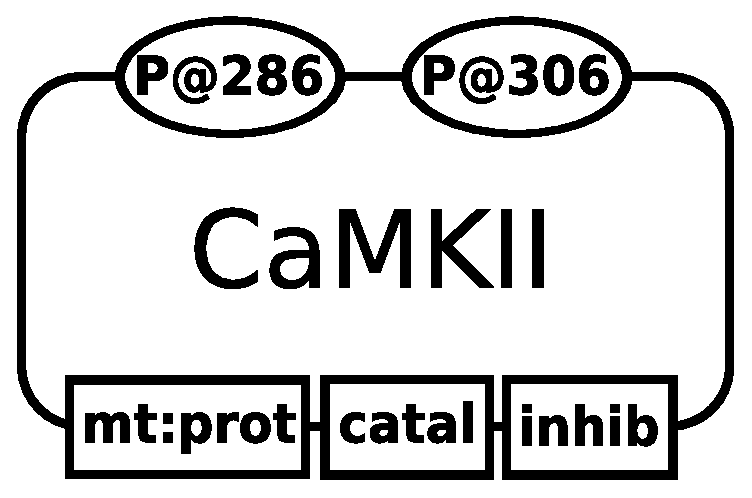
\includegraphics[scale = 0.8]{examples/macromolecule-CaMKII}
  \caption{An example representation of calcium/calmodulin kinase II EPN.}
  \label{fig:example-camkii}
\end{figure}

\fig{example-glur} represents the glutamate receptor in the open state, with both phosphorylation and glycosylation.  The entity carries two functional domains, the ligand-binding domain and the ion pore, and its chemical nature is presided.

\begin{figure}[H]
  \centering
  \includegraphics[scale = 0.8]{examples/macromolecule-GluR}
  \caption{An example of a glutamate receptor in the open state.}
  \label{fig:example-glur}
\end{figure}

%%% Local Variables: 
%%% mode: latex
%%% TeX-master: "../sbgn_PD-level1"
%%% End: 


\section{Referring to other Nodes}

Reference nodes handle links or relationships between elements of a map and sub-map. At present there is only one reference glyph, \glyph{tag}, which can be used in a map refered to by a \glyph{submap} (\sect{submap}) or as an auxilary unit on the \glyph{submap}. The \glyph{clone marker} can also provide additional reference mechanisms and is discussed below (\sect{cloneMarker}).

% $HeadURL$

\subsection{Glyph: \glyph{Tag}}
\label{sec:tag}

A \glyph{tag} is a named handle, or reference, to another EPN (\sect{EPNs}) or compartment (\sect{compartment}).  \glyph{Tags} are used to identify those elements in \glyph{submaps} (\sect{submap}).

\begin{glyphDescription}

\glyphSboTerm Not applicable.

\glyphContainer A \glyph{tag} is represented by a rectangle fused to an empty arrowhead, as illustrated in \fig{tag}.  The symbol should be linked to one and only one edge (\ie it should reference only one EPN or compartment).

\glyphLabel A \glyph{tag} is identified by a label placed in an unbordered box containing a string of characters.  The characters can be distributed on several lines to improve readability, although this is not mandatory.  The label box must be attached to the center of the container. The label may spill outside of the container.

\glyphAux A \glyph{tag} does not carry any auxiliary items. 

\end{glyphDescription}

\begin{figure}[H]
  \centering
  \includegraphics[scale = 0.3]{images/tag}
  \caption{The \PD glyph for \glyph{tag}.}
  \label{fig:tag}
\end{figure}




% The following is for [X]Emacs users.   Please leave in place.
% Local Variables:
% TeX-master: "../sbgn_PD-level1"
% End:



%%%%%%%%%%%%%%%%%%%%%%%%%%%%%%%%%%%%%%%%%%%%%%%%%%%%%%%%%%%%%%%%%%%%%%
%%%%%%%%%%%%%%%%%%%%%%%%%%%%%%%%%%%%%%%%%%%%%%%%%%%%%%%%%%%%%%%%%%%%%%
%%%%                   Containers
%%%%%%%%%%%%%%%%%%%%%%%%%%%%%%%%%%%%%%%%%%%%%%%%%%%%%%%%%%%%%%%%%%%%%%
%%%%%%%%%%%%%%%%%%%%%%%%%%%%%%%%%%%%%%%%%%%%%%%%%%%%%%%%%%%%%%%%%%%%%%

%\section{Container nodes}\label{sec:CNs}
\section{Defined sets of entity Pool nodes}

\subsection{Glyph: \glyph{Compartment}}
\label{sec:compartment}

A compartment is a logical or physical structure that contains entity pool nodes. An EPN can only belong to one compartment. Therefore, the ``same'' biochemical species located in two different compartments are in fact two different pools.

\begin{glyphDescription}

\glyphSboTerm  SBO:0000290 ! physical compartment


\glyphIncoming
None.



\glyphOutgoing
Zero or more \glyph{equivalence arcs} (\sect{equivalenceArc}).


\glyphContainer
A \glyph{compartment} is represented by a surface enclosed in a continuous border or located between continuous borders.
These borders should be noticeably thicker than the borders of the EPNs.
A compartment can take \textbf{any} shape.
A compartment must always be entirely enclosed.

\glyphLabel
A \glyph{compartment} is identified by a label that is  a string of characters that may be distributed on several lines to improve readability.
The label can be placed anywhere in the shape.
The label may extend outside of the shape.

\glyphAux
A \glyph{compartment} can carry one or more \glyph{units of information} (\sect{unitInfo}).
These can characterise the physical environment, such as pH, temperature or voltage.




\end{glyphDescription}

\begin{figure}[H]
  \centering
  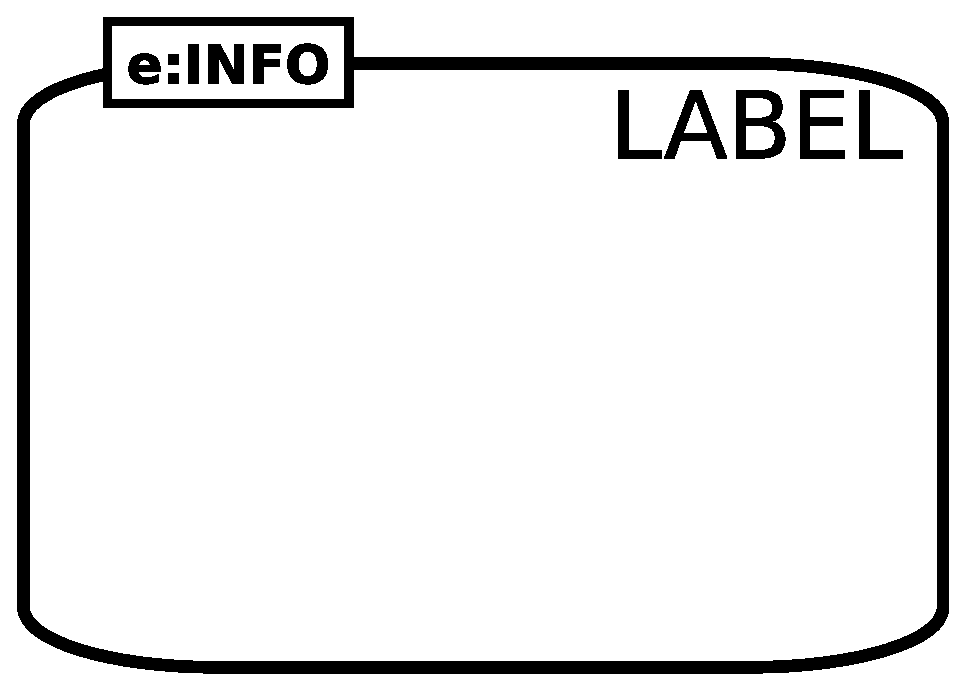
\includegraphics{images/compartment}
  \caption{The \PD glyph for \glyph{compartment}.}
  \label{fig:compartment}
\end{figure}

To allow more aesthetically pleasing and understandable maps, compartments are allowed to overlap each other visually, but it must be kept in mind that this does not mean the top compartment contains part of the bottom compartment.
\fig{overlap} shows two semantically equivalent placement of compartments:

\begin{figure}[H]
  \centering
  \includegraphics[scale = 0.5]{examples/compartment_overlapping}
  \caption{Overlapped compartments are permitted, but the overlap does not imply containment.}
  \label{fig:overlap}
\end{figure}

Overlapped (hidden) part of the compartment should not contain any object which could be covered by an overlapping compartment.
\fig{overlap-bad} illustrates the problem using an incorrect map.

\begin{figure}[H]
  \centering
  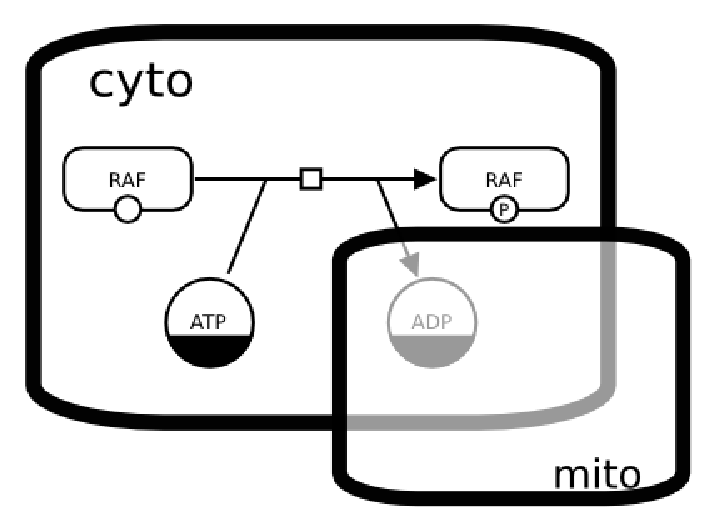
\includegraphics[scale = 0.8]{examples/compartment_overlapping_wrong}
  \caption{Example of an \textbf{incorrect} map.  Overlapped compartments must not obscure other objects.}
  \label{fig:overlap-bad}
\end{figure}

% It is important to note that a compartment never contains another compartment, but may surround it.  A key aspect of correctly drawing two ``adjacent'' compartments is that they are not separated by one line, but by \textbf{two} lines.  \fig{two-comp} provides an example of this in which a cell is shown made up of a nucleus surrounded by the cytoplasm.

% \begin{figure}[H]
%   \centering
%   \includegraphics[scale = 0.4]{examples/compartment-cell}
%  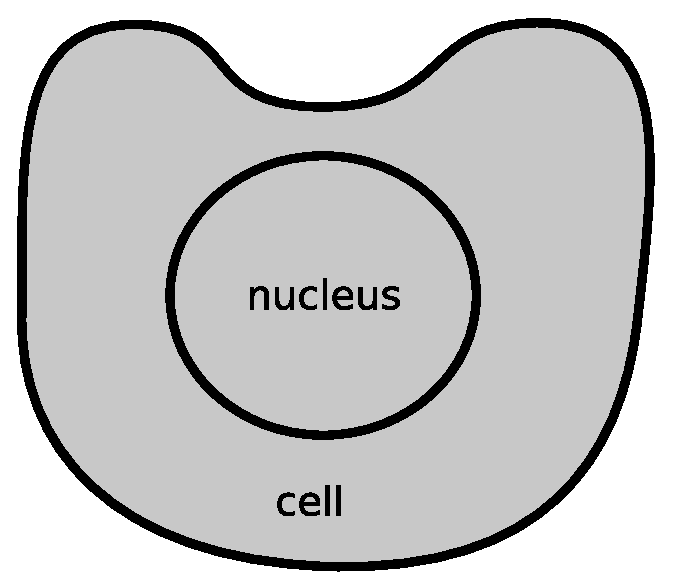
\includegraphics[scale = 0.4]{examples/compartment-cell-wrong}
%   \caption{Compartments can surround other compartments; in that case, both of the compartment's borders must still be shown, with the result that the separation is drawn as two lines. The left example is correct, with twoo disjoint compartments representing the ``cytoplasm'' and the ``nucleus''. The right example is incorrect. Indeed the compartments ``cell'' and ``nucleus'' would be disjoint, the latter only overlapping the former. As a result, the volume of the nucleus is duplicated.}
%   \label{fig:two-comp}
% \end{figure}

% The example diagram in \fig{three-comp} represents three adjacent compartments.  Two of the compartments carry units of information.  Notice that these units of information do not overlap multiple membrane boundaries.

% \begin{figure}[H]
%   \centering
%   \includegraphics[scale = 0.4]{examples/compartment-3comp}
%   \caption{Illustration of units of information and surrounding compartments.}
%   \label{fig:three-comp}
% \end{figure}

% The following is for [X]Emacs users.  Please leave in place.
% Local Variables:
% TeX-master: "../sbgn_PD-level1"
% End:


%%%%%%%%%%%%%%%%%%%%%%%%%%%%%%%%%%%%%%%%%%%%%%%%%%%%%%%%%%%%%%%%%%%%%%
%%%%%%%%%%%%%%%%%%%%%%%%%%%%%%%%%%%%%%%%%%%%%%%%%%%%%%%%%%%%%%%%%%%%%%
%%%%                   Submap
%%%%%%%%%%%%%%%%%%%%%%%%%%%%%%%%%%%%%%%%%%%%%%%%%%%%%%%%%%%%%%%%%%%%%%
%%%%%%%%%%%%%%%%%%%%%%%%%%%%%%%%%%%%%%%%%%%%%%%%%%%%%%%%%%%%%%%%%%%%%%

\section{Encapsulation}
\subsection{\glyph{Submap}}\label{sec:submap}

A \glyph{submap} is used to encapsulate a map (including all types of nodes and edges) within one glyph.
As such, it is not equivalent to an \glyph{omitted process} (\sect{omitted}).
The \glyph{submap} hides the content of this map to the users, and displays only \glyph{submap terminals} (\sect{submapTerminal}).
In the case of an SBGN description that is made available through a software tool, the map enclosed by the  \glyph{submap} may be available to the tool.
A user could then ask the tool to expand this map in a different canvas, for instance by clicking on the \glyph{submap}.
In the case of an SBGN description made available in a book or a website, the content of the map may be available on another page, possibly accessible via an hyperlink on the \glyph{submap}.

\begin{glyphDescription}

\glyphSboTerm
SBO:0000395 ! encapsulating process

\glyphIncoming
None.

\glyphOutgoing
None.

\glyphContainer
A \glyph{submap} is represented by a rectangular shape, to remind that it is fundamentally a process.

\glyphLabel
A \glyph{submap} is identified by a label that is an unbordered box containing a string of characters.
The characters may be distributed on several lines to improve readability.
The centre of the label must be placed on the centre of the shape.
The label may extend outside of the shape.

\glyphAux
A \glyph{submap} must carry one or more \glyph{submap terminals} (\sect{submapTerminal}), each linked to an \glyph{EPN} (\sect{EPNs}) or \glyph{compartment} (\sect{compartment}) of the map using an \glyph{equivalence arc} (\sect{equivalenceArc}).

\end{glyphDescription}

\begin{figure}
\begin{center}
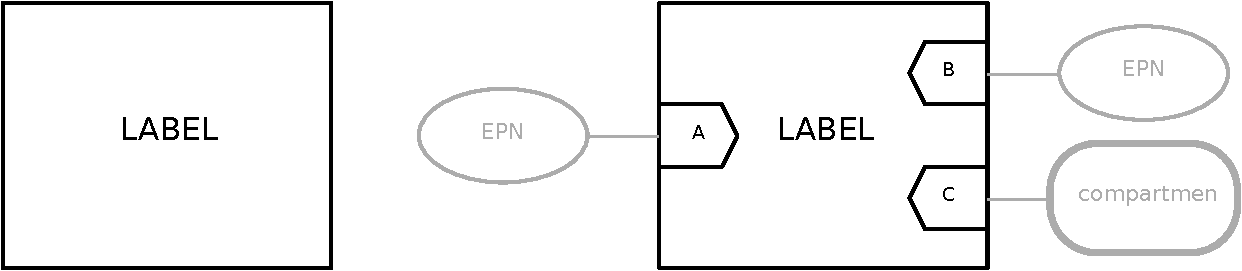
\includegraphics[scale=0.7]{images/build/submap.pdf}
\caption{The \PD glyph for \glyph{submap}, shown plain and unadorned on the left, and with three \glyph{submap terminals} on the right.}
\label{fig:submap}
\end{center}
\end{figure}

\fig{folded} represents a \glyph{submap} that encapsulates processes transforming glucose into fructose-6-phosphate.
The \glyph{submap} carries five \glyph{submap terminals}, four linked to \glyph{EPNs} and one linked to a \glyph{compartment}.
The latter is particularly important in the case of \glyph{EPNs} present only in a \glyph{compartment} enclosed in a \glyph{submap}, and that are not linked to \glyph{submap terminals} themselves.
Note that the \glyph{submap terminals} do not allow defining a ``direction'' for the flux of the processes enclosed in the \glyph{submap}, which is solely determined by the context as in \fig{folded}.

\begin{figure}
\begin{center}
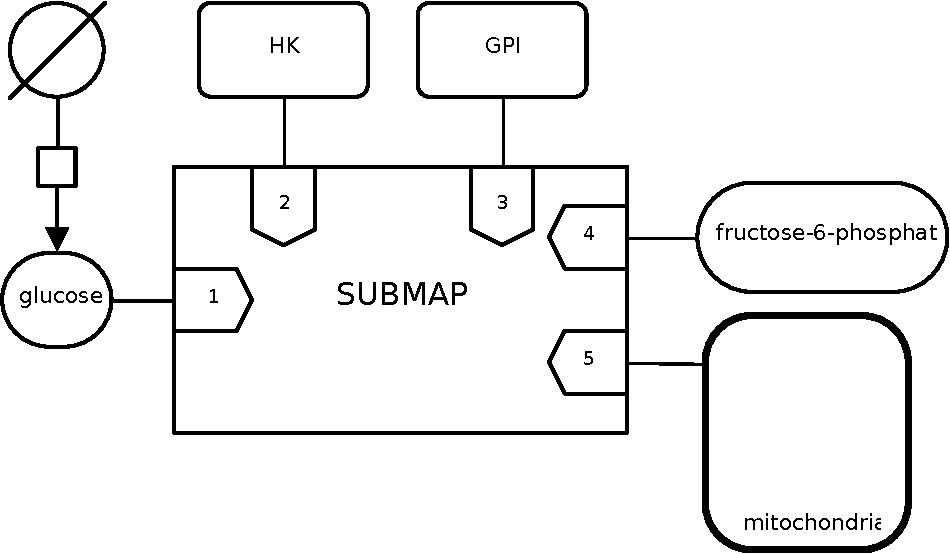
\includegraphics[scale=0.8]{images/build/submap_folded_example.pdf}
\caption{Example of a \glyph{submap} encapsulating processes that transform glucose into fructose-6-phosphate.
The map enclosed by the \glyph{submap} is shown in \fig{unfolded}, whose \glyph{tags} are referred to by the \glyph{submap terminals} decorating the present \glyph{submap} glyph.
}
\label{fig:folded}
\end{center}
\end{figure}

The map in \fig{unfolded} represents the map enclosed in the \glyph{submap} of \fig{folded}.
Note that the tag 5 links the mitochondria \glyph{compartment} in this map to the mitochondria \glyph{compartment} of the main map in \fig{unfolded}.

The \glyph{compartment} containing glucose-6-phosphate is implicitly defined as the same as the \glyph{compartment} containing glucose and fructose-6-phosphate.
There is no ambiguity because if glucose and fructose-6-phosphate were in different \glyph{compartments}, at least one of them would have been linked to a \glyph{submap terminal} of the \glyph{submap} of \fig{folded}.

\begin{figure}
\begin{center}
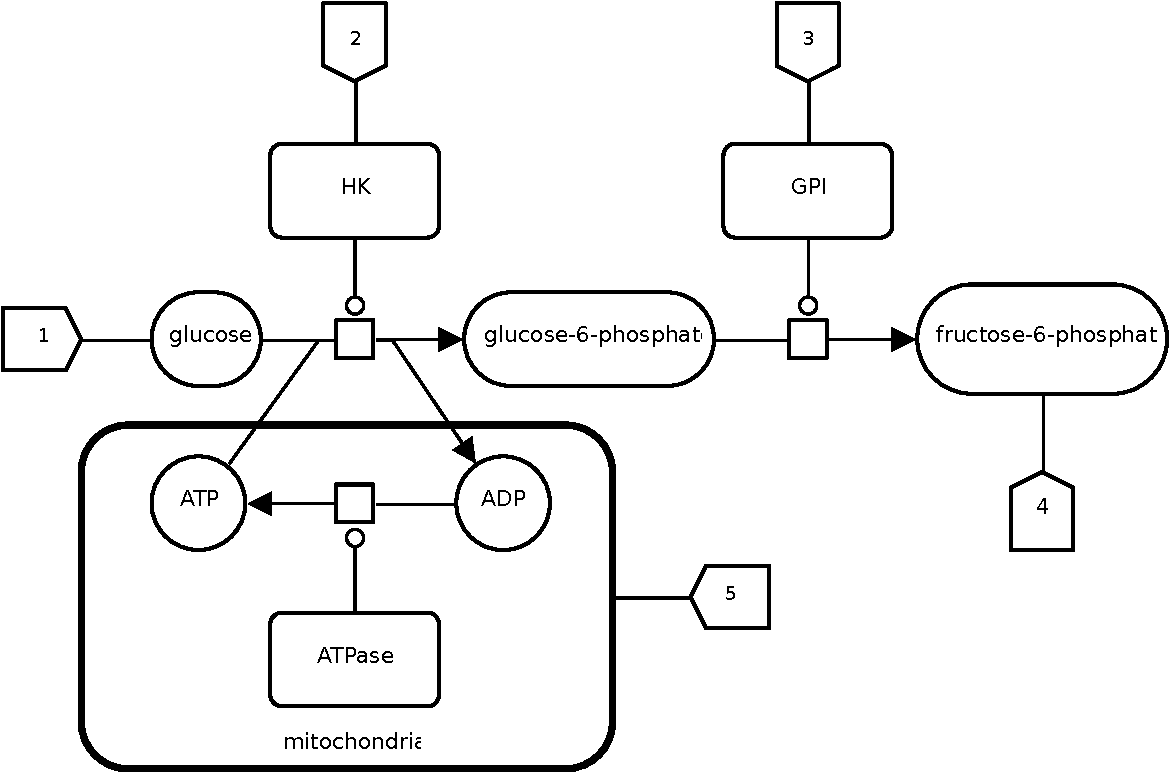
\includegraphics[scale=0.8]{images/build/submap_unfolded_example.pdf}
\caption{Example of a map with \glyph{tags}, showing that it is enclosed in a \glyph{submap} of another map (here, the one of \fig{folded}).}
\label{fig:unfolded}
\end{center}
\end{figure}



%%%%%%%%%%%%%%%%%%%%%%%%%%%%%%%%%%%%%%%%%%%%%%%%%%%%%%%%%%%%%%%%%%%%%%
%%%%%%%%%%%%%%%%%%%%%%%%%%%%%%%%%%%%%%%%%%%%%%%%%%%%%%%%%%%%%%%%%%%%%%
%%%%                   Process nodes
%%%%%%%%%%%%%%%%%%%%%%%%%%%%%%%%%%%%%%%%%%%%%%%%%%%%%%%%%%%%%%%%%%%%%%
%%%%%%%%%%%%%%%%%%%%%%%%%%%%%%%%%%%%%%%%%%%%%%%%%%%%%%%%%%%%%%%%%%%%%%

\section{Process nodes}\label{sec:PNs}

Process nodes represent processes that transform one or several entity pools into one or several entity pools, identical or different.  \SBGNPDLone defines a generic \glyph{process} (\sect{process}), as well as five more specific ones: the \glyph{omitted process} (\sect{omitted}), the \glyph{uncertain process} (\sect{uncertain}), the \glyph{association} (\sect{association}), the \glyph{dissociation} (\sect{dissociation}), and the \glyph{phenotype} (\sect{phenotype}).  In future levels of the SBGN \PDl, more processes may be defined.  (One can even envision the development of a controlled vocabulary of processes, as is done now for \glyph{EPNs}; see \sect{CVs}.)

% $HeadURL$

%%%%%%%%%%%%%%%%%%%%%%%%%%%%%%%%%%%%%%%%%%%%%%%%%%%%%%%%%%%%%%%%%%%%%%
%%                     Process
%%%%%%%%%%%%%%%%%%%%%%%%%%%%%%%%%%%%%%%%%%%%%%%%%%%%%%%%%%%%%%%%%%%%%%

\subsection{Glyph: \glyph{Process}}
\label{sec:process}

A process transforms a set of entity pools (represented by \glyph{EPNs} in \SBGNPDLone) into another set of entity pools.

\begin{glyphDescription}

\glyphSboTerm SBO:0000375 ! process

\glyphOrigin One or several \glyph{consumption} arcs (\sect{consumption}) or one or several \glyph{production} arcs (\sect{production}).

\glyphTarget One or several \glyph{production} arcs (\sect{production}).

\glyphNode A process is represented by a square box linked to two connectors, small arcs attached to the centers of opposite sides. The consumption (\sect{consumption}) and production (\sect{production}) arcs are linked to the extremities of those connectors. The modulatory arcs (\sect{arcs}) point to the other two sides of the box. A \glyph{process} connected to \glyph{production} arcs on opposite sides is a reversible process. 

\end{glyphDescription}

\begin{figure}[H]
  \centering
  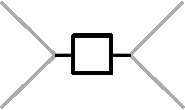
\includegraphics[scale = 0.4]{images/process}
  \caption{The \PD glyph for \glyph{process}.}
  \label{fig:process}
\end{figure}

A process is the basic process node in SBGN.  It describes a process that transforms a given set of biochemical entities---macromolecules, simple chemicals or unspecified entities---into another set of biochemical entities.  Such a transformation might imply modification of covalent bonds (conversion), modification of the relative position of constituents (conformational process) or movement from one compartment to another (translocation).

A cardinality label may be associated with \glyph{consumption} (\sect{consumption}) or \glyph{production} (\sect{production}) arcs to indicate the stoichiometry of the process.  This label becomes a requirement when the exact composition of the number of copies of the inputs or outputs to a reaction are ambiguous in the map.

A process is regarded as reversible if both `sides' of the process are connected to \glyph{production} arcs (see section \ref{sec: semantics reversible procs}).

The example in \fig{trans-phos} illustrates the use of a \glyph{process} node to represent the phosphorylation of a protein in a \PD.

\begin{figure}[H]
  \centering
  
\includegraphics[scale = 0.3]{examples/process-phosphorylation}
  \caption{Phosphorylation of the protein MAP kinase.}
  \label{fig:trans-phos}
\end{figure}

The example in \fig{trans-react} illustrates the use of a \glyph{process} node to represent a reaction between two reactants that generates three products. 

\begin{figure}[H]
  \centering
  \includegraphics[scale = 0.3]{examples/process-reaction}
  \caption{Reaction between ATP and fructose-6-phosphate to produce fructose-1,6-biphosphate, ADP and a proton.}
  \label{fig:trans-react}
\end{figure}

The example in \fig{trans-trans} illustrates the use of a \glyph{process} node to represent a translocation. The large round-cornered rectangle represents a compartment border (see \sect{compartment}).

\begin{figure}[H]
  \centering
  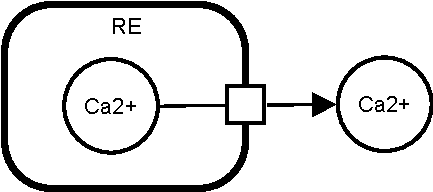
\includegraphics[scale = 0.3]{examples/process-translocation}
  \caption{Translocation of calcium ion out of the endoplasmic reticulum. Note that the \glyph{process} does not have to be located on the boundary of the \glyph{compartment}. A \glyph{process} is not attached to any \glyph{compartment}.}
  \label{fig:trans-trans}
\end{figure}

The example in \fig{trans-reverse} illustrates the use of a \glyph{process} node to represent the reversible opening and closing of an ionic channel in a \PD.

\begin{figure}[H]
  \centering
  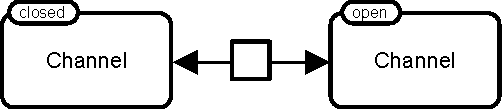
\includegraphics[scale = 0.3]{examples/process-reversible}
  \caption{Reversible opening and closing of an ionic channel.}
  \label{fig:trans-reverse}
\end{figure}

When such a reversible process is asymmetrically modulated, it must be represented by two different processes in a \PD.  \fig{trans-mod} illustrates the use of two \glyph{process} nodes to represent the reversible activation of a G-protein coupled receptor.  In the absence of any effector, an equilibrium exists between the inactive and active forms.  The agonist stabilises the active form, while the inverse agonist stabilises the inactive form.

\begin{figure}[H]
  \centering
  \includegraphics[scale = 0.3]{examples/process-modulated}
  \caption{The reversible activation of a G-protein coupled receptor.}
  \label{fig:trans-mod}
\end{figure}

The example in \fig{trans-dim} presents the conversion of two galactoses into a lactose.  Galactoses are represented by only one \glyph{simple chemical}, the cardinality being carried by the \glyph{consumption} arc.

\begin{figure}[H]
  \centering
  
\includegraphics[scale = 0.3]{examples/process-dimerisation}
  \caption{Conversion of two galactoses into a lactose.}
  \label{fig:trans-dim}
\end{figure}




% The following is for [X]Emacs users.  Please leave in place.
% Local Variables:
% TeX-master: "../sbgn_PD-level1"
% End:

%%%%%%%%%%%%%%%%%%%%%%%%%%%%%%%%%%%%%%%%%%%%%%%%%%%%%%%%%%%%%%%%%%%%%%
%%                     Omitted Process
%%%%%%%%%%%%%%%%%%%%%%%%%%%%%%%%%%%%%%%%%%%%%%%%%%%%%%%%%%%%%%%%%%%%%%
%\color{blue}
\subsection{Glyph: \glyph{Omitted process}}\label{sec:omitted}

Omitted processes are processes that are known to exist, but are omitted from the map for the sake of clarity or parsimony. A single \glyph{omitted process} can represent any number of actual processes. For instance, one may want to represent a long chain of processes leading from one biochemical compound to another, without detailing all steps, but highlighting the fact that this is not a direct transformation.  The \glyph{omitted process} is different from a \glyph{submap} (\sect{submap}). While a \glyph{submap} references to an explicit content, that is hidden in the main map, the \glyph{omitted process} does not ``hide'' anything within the context of the map, and cannot be ``unfolded''. An \glyph{omitted process} is represented by a \glyph{process} in which the square box contains a two parallel slanted lines oriented northwest-to-southeast and separated by an empty space.

\begin{figure}[H]
  \centering
  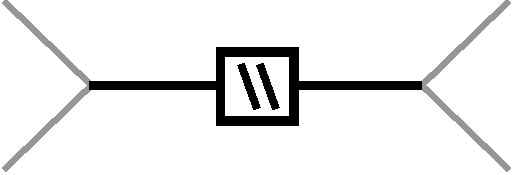
\includegraphics[scale = 0.5]{images/omitted}
  \caption{The \PD glyph for \glyph{omitted process}.}
  \label{fig:omitted}
\end{figure}




\subsection{Glyph: \glyph{Uncertain process}}
\label{sec:uncertain}

Uncertain processes are processes that may not exist. A single \glyph{uncertain process} can represent any number of actual processes.

\begin{glyphDescription}

\glyphSboTerm
SBO:0000396 ! uncertain process

\corr{\glyphOrigin
One or several \glyph{consumption} arcs (\sect{consumption}) or one or several \glyph{production} arcs (\sect{production}).
}{
\glyphIncoming
One or more \glyph{consumption} arcs (\sect{consumption})\footnote{Zero \glyph{consumption arcs} are allowed in the case of a reversible process.}, zero or more \glyph{modulation} arcs (\sect{modulations}).
}

\corr{\glyphTarget
One or several \glyph{production} arcs (\sect{production}).
}{
\glyphOutgoing
One or more \glyph{production} arcs (\sect{production}).
}

\glyphContainer
A \glyph{process} is represented by a square shape containing a question mark.
The shape is linked to two ports, that are small arcs attached to the centres of opposite sides of the shape, as shown in \fig{uncertain}.
The incoming \glyph{consumption} (\sect{consumption}) and outgoing \glyph{production} (\sect{production}) arcs are linked to the extremities of those ports.

The \glyph{modulation arcs} (\sect{modulations}) point to the other two sides of the shape.

\glyphLabel
\corr{An \glyph{uncertain process} is not identified by any label}{None}.

\glyphAux
\corr{An \glyph{uncertain process} does not carry any auxiliary items}{None}.

\end{glyphDescription}

\begin{figure}[H]
  \centering
  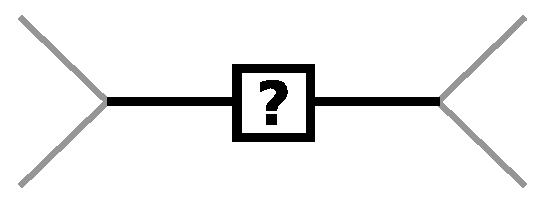
\includegraphics{images/uncertain}
  \caption{The \PD glyph for an \glyph{uncertain process}.}
  \label{fig:uncertain}
\end{figure}

\subsection{Glyph: \glyph{Association}}
\label{sec:association}

The \glyph{association} between one or more \glyph{EPNs} represents the non-covalent binding of the biological entities represented by those \glyph{EPNs} into a larger complex.

\begin{glyphDescription}

\glyphSboTerm
SBO:0000177 ! non-covalent binding

\corr{
\glyphOrigin One or more \glyph{consumption} arcs (\sect{consumption}).
}{
\glyphIncoming
One or more \glyph{consumption} arcs (\sect{consumption}), zero or more \glyph{modulation} arcs (\sect{modulations}).
}

\corr{
\glyphTarget  One \glyph{production} arc (\sect{production}).
One or several \glyph{production} arcs (\sect{production}).
}{
\glyphOutgoing
One \glyph{production} arc (\sect{production}).
}

\glyphContainer
An \glyph{association} is represented by a circular filled shape.
The shape is linked to two ports, that are small arcs attached to the centres of opposite sides of the shape, as shown in \fig{association}.
The incoming \glyph{consumption} (\sect{consumption}) and outgoing \glyph{production} (\sect{production}) arcs are linked to the extremities of those ports.

The \glyph{modulation arcs} (\sect{modulations}) point to the other two sides of the shape.

\glyphLabel
\corr{A \glyph{association} is not identified by any label}{None}.

\glyphAux
\corr{A \glyph{association} does not carry any auxiliary items}{None}.

\end{glyphDescription}

\begin{figure}[H]
  \centering
  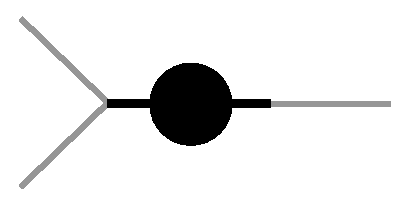
\includegraphics{images/association}
  \caption{The \PD glyph for \glyph{association}.}
  \label{fig:association}
\end{figure}

The example in \fig{assoc-cyclin} illustrates the association of cyclin and CDC2 kinase into the Maturation Promoting Factor.

\begin{figure}[H]
  \centering
  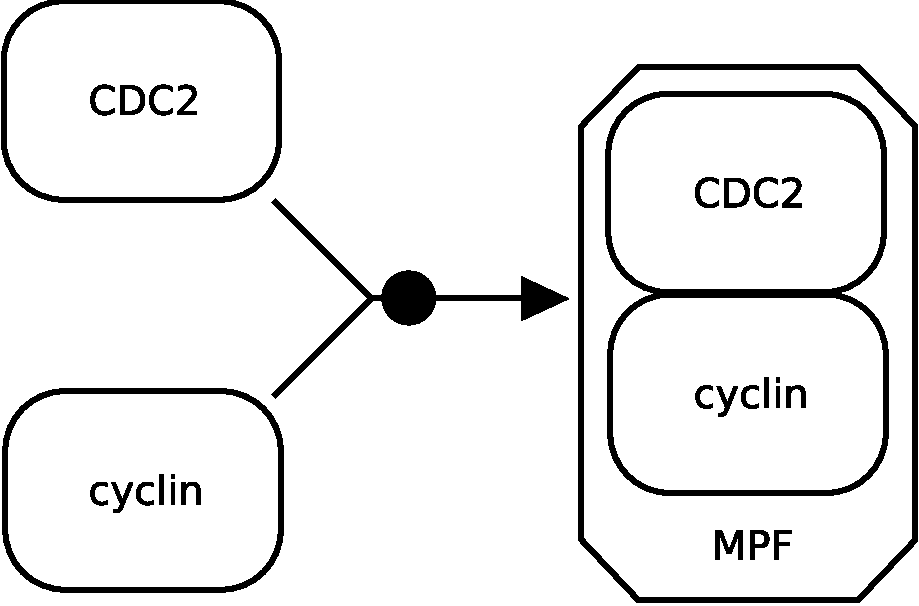
\includegraphics[scale = 0.8]{examples/association-MPF}
  \caption{Association of cyclin and CDC2 kinase into the Maturation Promoting Factor.}
  \label{fig:assoc-cyclin}
\end{figure}

\fig{assoc-unamed} gives an example illustrating the association of a pentameric macromolecule (a nicotinic acetylcholine receptor) with a simple chemical (the local anesthetic chlorpromazin) in an unnamed complex.

\begin{figure}[H]
  \centering
  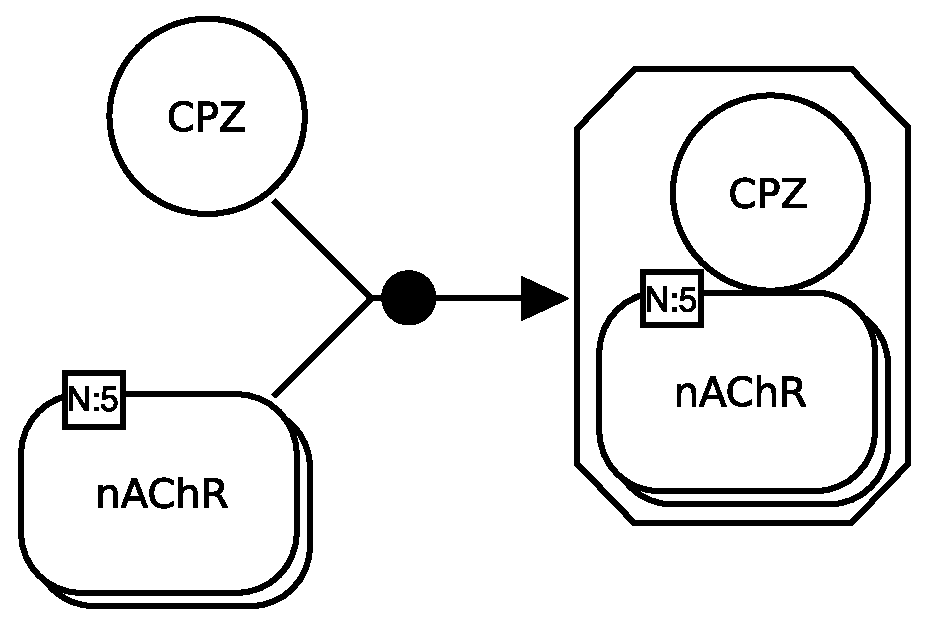
\includegraphics[scale = 0.8]{examples/association-unamed}
  \caption{The association of a pentameric macromolecule with a simple chemical in an unnamed complex.}
  \label{fig:assoc-unamed}
\end{figure}

An association does not necessarily result in the formation of a \glyph{complex}; it can also produce a \glyph{multimer}, or a \glyph{macromolecule} (although the latter case is semantically borderline).  \fig{assoc-multi} gives an example of this, using the formation of hemoglobin.

\begin{figure}[H]
  \centering
  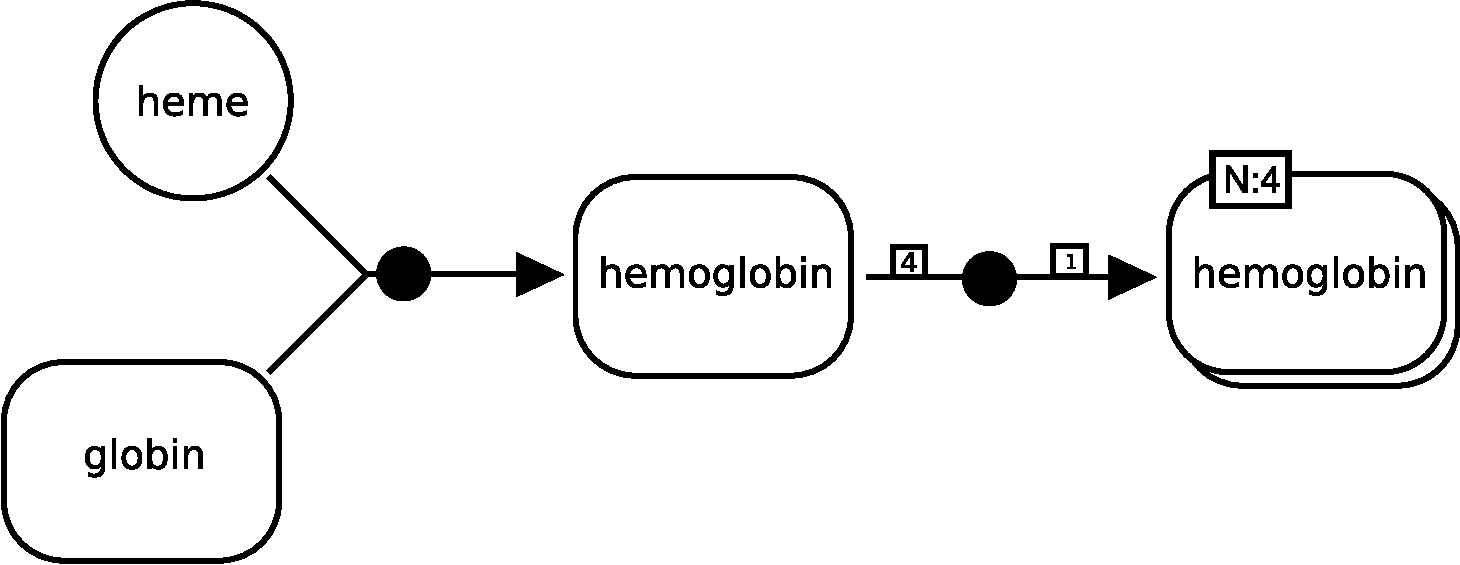
\includegraphics[scale = 0.8]{examples/association-multimerisation}
  \caption{Formation of hemoglobin.}
  \label{fig:assoc-multi}
\end{figure}

% The following is for [X]Emacs users.  Please leave in place.
% Local Variables:
% TeX-master: "../sbgn_PD-level1"
% End:

%%%%%%%%%%%%%%%%%%%%%%%%%%%%%%%%%%%%%%%%%%%%%%%%%%%%%%%%%%%%%%%%%%%%%%
%%                     Dissociation
%%%%%%%%%%%%%%%%%%%%%%%%%%%%%%%%%%%%%%%%%%%%%%%%%%%%%%%%%%%%%%%%%%%%%%
%\color{blue}
\subsection{Glyph: \glyph{Dissociation}}\label{sec:dissociation}

The dissociation of an \glyph{EPN} into one or more \glyph{EPNs} represents the rupture of a non-covalent binding between the biological entities represented by those \glyph{EPNs}.

\begin{glyphDescription}
 \glyphSboTerm SBO:0000180 ! dissociation.
 \glyphOrigin One \glyph{consumption} arc (\sect{consumption}).
 \glyphTarget  One or more \glyph{production} arc (\sect{production}).
 \glyphNode A \glyph{dissociation} between several entities is represented by two concentric circles. A simple empty disc could be, in some cases, confused with the \glyph{catalysis} (section \sect{catalysis}). Moreover, the existence of two circles reminds the dissociation, by contrast with the filled disc of the \glyph{association} (\sect{association}).
 \end{glyphDescription}


\begin{figure}[H]
  \centering
  
\includegraphics[scale = 0.5]{images/dissociation}
  \caption{The \PD glyph for \glyph{dissociation}.}
  \label{fig:dissociation}
\end{figure}

The example in \fig{dissoc-ribo} illustrates the dissociation of the small and large ribosomal subunits from a messenger RNA.

\begin{figure}[H]
  \centering
  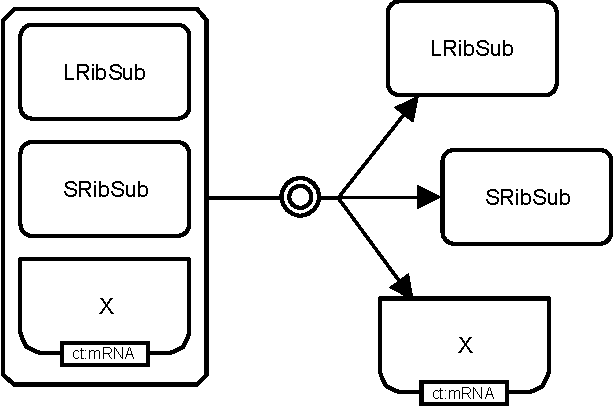
\includegraphics[scale = 0.3]{examples/dissociation-ribosome}
  \caption{Dissociation of the small and large ribosomal subunits from a messenger RNA.}
  \label{fig:dissoc-ribo}
\end{figure}

\subsection{Glyph: \glyph{Phenotype}}
\label{sec:phenotype}

A biochemical network can generate phenotypes or affect biological processes.
Such processes can take place at different levels and are independent of the biochemical network itself.
To represent these processes in a map, \PD defines the \glyph{phenotype} glyph.

\begin{glyphDescription}

\glyphSboTerm
SBO:0000358 ! phenotype


\glyphIncoming
One or more \glyph{modulation} arcs (\sect{modulations}).



\glyphOutgoing
None.


\glyphContainer
A \glyph{phenotype} is represented by an elongated hexagonal shape, as shown in \fig{phenotype}.

\glyphLabel
A \glyph{phenotype} is identified by a label that is  a string of characters that may be distributed on several lines to improve readability.
The centre of the label must be placed on the centre of the shape.
The label may extend outside of the shape.

\glyphAux 
None.

\end{glyphDescription}

\begin{figure}[H]
  \centering
  \includegraphics{images/build/phenotype.pdf}
  \caption{The \PD glyph for \glyph{phenotype}.}
  \label{fig:phenotype}
\end{figure}

% The following is for [X]Emacs users.   Please leave in place.
% Local Variables:
% TeX-master: "../sbgn_PD-level1"
% End:


%%%%%%%%%%%%%%%%%%%%%%%%%%%%%%%%%%%%%%%%%%%%%%%%%%%%%%%%%%%%%%%%%%%%%%
%%%%%%%%%%%%%%%%%%%%%%%%%%%%%%%%%%%%%%%%%%%%%%%%%%%%%%%%%%%%%%%%%%%%%%
%%%%                  Arcs
%%%%%%%%%%%%%%%%%%%%%%%%%%%%%%%%%%%%%%%%%%%%%%%%%%%%%%%%%%%%%%%%%%%%%%
%%%%%%%%%%%%%%%%%%%%%%%%%%%%%%%%%%%%%%%%%%%%%%%%%%%%%%%%%%%%%%%%%%%%%%

\section{Arcs}\label{sec:arcs}

Arcs are lines that link \glyph{EPNs} and \glyph{PNs} together.  The symbols attached to their extremities indicate their semantics.

\subsection{Glyph: \glyph{Consumption}}
\label{sec:consumption}

\glyph{Consumption} is the arc used to represent the fact that an entity pool is consumed by a process, but is not produced by the process.

\begin{glyphDescription}

\glyphSboTerm
SBO:0000394 ! consumption

\glyphOrigin
One \glyph{EPN} (\sect{EPNs}).

\glyphTarget
One \glyph{process node} (\sect{PNs}).

\glyphSymbol
No particular symbol is used to represent a \glyph{consumption}, as shown in \fig{consumption}.

\end{glyphDescription}

\begin{figure}[H]
  \centering
  \includegraphics{images/build/consumption.pdf}
  \caption{The \PD glyph for \glyph{consumption}.}
  \label{fig:consumption}
\end{figure}

A cardinality label may be associated with \glyph{consumption} (\sect{consumption}) or \glyph{production} (\sect{production}) arcs, indicating the stoichiometry of a process.
This label is a number enclosed in a rectangular container with one of the long sides adjacent to the \glyph{consumption} arc.
The cardinality is required to eliminate ambiguity when the exact composition, or the number of copies, of the inputs or outputs to a reaction are ambiguous from the map.
An example is a multimer of six subunits dissociating into two monomers and two dimers.
Without stoichiometry labels another result, such as four monomers and one dimer could be inferred.
Once assigned to one arc connecting to a process node, cardinality should be represented on all \glyph{consumption} and \glyph{production} arcs connected to that process node to avoid misinterpretation.

Omitted cardinality on one edge only should not be treated as cardinality of one, but as an unspecified cardinality.
In most cases, the exact value may be derived from the context, but unless cardinality is explicitly shown, it should be considered as unspecified.
In the case where the stoichiometry of some part of the process is not known, or undefined, a question mark ("?") should be used within the cardinality label of the corresponding arcs.

\subsection{Glyph: \glyph{Production}}
\label{sec:production}

\glyph{Production} is the arc used to represent the fact that an entity pool is produced by a process. In the case of a reversible process, the \glyph{production} arc \corr{also acts as a \glyph{consumption} arc}{represents both a consumption and a production}.

\begin{glyphDescription}

\glyphSboTerm
SBO:0000393 ! production

\glyphOrigin
\corr{Any}{One} \glyph{process node} (\sect{PNs}).

\glyphTarget
\corr{Any}{One} \glyph{EPN} (\sect{EPNs}).

\glyphSymbol
The target extremity of a \glyph{production} carries a filled arrowhead, as shown in \fig{production}.

\end{glyphDescription}

\begin{figure}[H]
  \centering
  \includegraphics{images/production}
  \caption{The \PD glyph for \glyph{production}.}
  \label{fig:production}
\end{figure}

A cardinality label may be associated with a \glyph{production} arc, indicating the stoichiometry of a process.

\fig{prod-card} illustrates the use of \corr{consumption/production}{\glyph{consumption}/\glyph{production}} arc cardinality labels to represent the stoichiometry of a process.

\begin{figure}[H]
  \centering
  \includegraphics[scale = 0.6]{examples/stoichEx1}
  \caption{Cardinality for production arcs.
  \add{The process on the top is wrong as the stoichiometry is not represented, which leads to ambiguity.}}
  \label{fig:prod-card}
\end{figure}

% The following is for [X]Emacs users.  Please leave in place.
% Local Variables:
% TeX-master: "../sbgn_PD-level1"
% End:

\subsection{Glyph: \glyph{Modulation}}
\label{sec:modulation}

% A modulation affects the flux of a process
% represented by the target process. Such a modulation can affect the
% process \textbf{positively or negatively}, or even both ways depending on the
% conditions, for instance the concentration of the intervening
% participants. A \glyph{modulation} can also be used when one does not know the precise direction of the effect.

A general modulation where the exact nature of the modulation is not specified or not known.
The \glyph{modulation} glyph can be used when one does not know the precise direction of the effect.

\begin{glyphDescription}

\glyphSboTerm
SBO:0000168 ! control

\glyphOrigin
One \glyph{EPN} (\sect{EPNs}) or  \glyph{logical operator} (\sect{logic}).

\glyphTarget
One \glyph{process node} (\sect{PNs}).

\glyphSymbol
The target extremity of a \glyph{modulation} carries an empty diamond, as shown in \fig{modulation}.

\end{glyphDescription}

\begin{figure}[H]
  \centering
  \includegraphics{images/build/modulation.pdf}
  \caption{The \PD glyph for \glyph{modulation}.}
  \label{fig:modulation}
\end{figure}

\fig{modul-nico} represents the effect of nicotine on the process between closed and open states of a nicotinic acetylcholine receptor. High concentrations of nicotine open the receptor while low concentrations can desensitize it without opening.

\begin{figure}[H]
  \centering
  \includegraphics[scale = 0.8]{images/build/modulation_nAChR_example.pdf}
  \caption{Modulation of nicotinic receptor opening by nicotine.}
  \label{fig:modul-nico}
\end{figure}

\subsection{Glyph: \glyph{Stimulation}}
\label{sec:stimulation}

A stimulation affects \textbf{positively} the flux of a process represented by the target process.
This stimulation can be, for instance, a catalysis or a positive allosteric regulation. Note that \glyph{catalysis} exists independently in SBGN, see \sect{catalysis}.

\begin{glyphDescription}

\glyphSboTerm
SBO:0000170 ! stimulation

\glyphOrigin
One \glyph{EPN} (\sect{EPNs}) or  \glyph{logical operator} (\sect{logic}).

\glyphTarget
One \glyph{process node} (\sect{PNs}).

\glyphSymbol
The target extremity of a \glyph{stimulation} carries an empty arrowhead, as shown in \fig{stimulation}.

\end{glyphDescription}

\begin{figure}[H]
  \centering
  \includegraphics{images/build/stimulation.pdf}
  \caption{The \PD glyph for \glyph{stimulation}.}
  \label{fig:stimulation}
\end{figure}

%%%%%%%%%%%%%%%%%%%%%%%%%%%%%%%%%%%%%%%%%%%%%%%%%%%%%%%%%%%%%%%%%%%%%%
%%                     Catalysis
%%%%%%%%%%%%%%%%%%%%%%%%%%%%%%%%%%%%%%%%%%%%%%%%%%%%%%%%%%%%%%%%%%%%%%
%\color{blue}
\subsection{Glyph: \glyph{Catalysis}}\label{sec:catalysis}

A catalysis is a particular case of stimulation, where the effector affects
positively the flux of a process represented by the target process. The positive effect on the process is due to the lowering of the activation energy of a reaction. The target extremity of a \glyph{catalysis} carries an empty circle.

\begin{figure}[H]
  \centering
  \includegraphics[scale = 0.5]{images/catalysis}
  \caption{The \PD glyph for \glyph{catalysis}.}
  \label{fig:catalysis}
\end{figure}

The example in \fig{catalysis-MAPK} illustrates the use of \glyph{catalysis} arc to represent the effect of MAPKK on the phophorylation of MAPK.

\begin{figure}[H]
  \centering
  \includegraphics[scale = 0.5]{images/catalysis-MAPK}
  \caption{MAPKK catalyses the phosphorylation of MAPK.}
  \label{fig:catalysis-MAPK}
\end{figure}

\subsection{Glyph: \glyph{Inhibition}}
\label{sec:inhibition}

An inhibition \textbf{negatively} affects the flux of a process represented by the target process.
This inhibition can be, for instance, a competitive inhibition or an allosteric inhibition.

\begin{glyphDescription}

\glyphSboTerm
SBO:0000169 ! inhibition

\glyphOrigin
One \glyph{EPN} (\sect{EPNs}) or \glyph{logical operator} (\sect{logic}).

\glyphTarget
One \glyph{process node} (\sect{PNs}).

\glyphSymbol
The target extremity of an \glyph{inhibition} carries a bar perpendicular to the arc, as shown in \fig{inhibition}.

\end{glyphDescription}

\begin{figure}[H]
  \centering
  \includegraphics{images/build/inhibition.pdf}
  \caption{The \PD glyph for \glyph{inhibition}.}
  \label{fig:inhibition}
\end{figure} 

\subsection{Glyph: \glyph{Necessary stimulation}}
\label{sec:necessary_stim}

A necessary stimulation is one that is necessary for a process to take place. A process modulated by a necessary stimulation can only occur when this necessary stimulation is active.

\begin{glyphDescription}

\glyphSboTerm
SBO:0000171 ! necessary stimulation

\glyphOrigin
One \glyph{EPN} (\sect{EPNs}) or \glyph{logical operator} (\sect{logic}).

\glyphTarget
One \glyph{process node} (\sect{PNs}).

\glyphSymbol
The target extremity of a \glyph{necessary stimulation} carries an open arrowhead (to remind that it is a \glyph{stimulation}) coming after a larger perpendicular bar, as shown in \fig{Necessary Stimulation}.

\end{glyphDescription}

\begin{figure}[H]
  \centering
  \includegraphics{images/build/necessary_stim.pdf}
  \caption{The \PD glyph for \glyph{Necessary Stimulation}.}
  \label{fig:Necessary Stimulation}
\end{figure}

The example in \fig{necessary_stim-gene} below describes the transcription of a gene~X, that is the creation of a messenger RNA~X triggered by the gene~X.  The creation of the protein~X is then triggered by the mRNA~X.  (Note that the same example could be represented using the gene as reactant and product, although it is semantically different.)

\begin{figure}[H]
  \centering
  \includegraphics[scale = 0.8]{images/build/necessary_stim_genetic_example.pdf}
  \caption{The creation of a messenger RNA~X triggered by the gene~X.}
  \label{fig:necessary_stim-gene}
\end{figure}

The example in \fig{necessary_stim-calcium} below describes the transport of calcium ions out of the endoplasmic reticulum. Without IP3 receptor, there is no calcium flux, therefore, one cannot use a \glyph{stimulation}.
The \glyph{necessary stimulation} instead represents the necessity for the receptor to be present for the transport to take place.

\begin{figure}[H]
  \centering
  \includegraphics[scale = 0.8]{images/build/necessary_stim_transport_example.pdf}
  \caption{The transport of calcium ions out of the endoplasmic reticulum into the cytosol. Note that IP3R crosses both compartment boundaries. This is allowed, but the Macromolecule should only belong to one of the compartments see section \ref{sec: unresolved multi-comp ents} for more discussion of this issue.}
  \label{fig:necessary_stim-calcium}
\end{figure}

%%%%%%%%%%%%%%%%%%%%%%%%%%%%%%%%%%%%%%%%%%%%%%%%%%%%%%%%%%%%%%%%%%%%%%
%%                     Logic arc
%%%%%%%%%%%%%%%%%%%%%%%%%%%%%%%%%%%%%%%%%%%%%%%%%%%%%%%%%%%%%%%%%%%%%%
%\color{blue}
\subsection{Glyph: \glyph{Logic arc} }\label{sec:logicArc}

\glyph{Logic arc} is used to represent the fact that an entity influences
the outcome of a logic operator. 

\begin{glyphDescription}
 \glyphSboTerm SBO:0000398 ! logical relationship.
 \glyphOrigin Any \glyph{EPN} (\sect{EPNs}) or \glyph{logical operator} (\sect{logic}).
 \glyphTarget Any \glyph{logical operator} (\sect{logic}).
 \glyphEndPoint No particular symbol is used to represent a logic arc.
 \end{glyphDescription}

\begin{figure}[H]
  \centering
  \includegraphics[scale = 0.4]{images/logicArc}
  \caption{The \PD glyph for \glyph{logic arc}.}
  \label{fig:logicArc}
\end{figure}

%%%%%%%%%%%%%%%%%%%%%%%%%%%%%%%%%%%%%%%%%%%%%%%%%%%%%%%%%%%%%%%%%%%%%%
%%                     Equivalence Arc
%%%%%%%%%%%%%%%%%%%%%%%%%%%%%%%%%%%%%%%%%%%%%%%%%%%%%%%%%%%%%%%%%%%%%%
%\color{blue}
\subsection{Glyph: \glyph{Equivalence arc} }\label{sec:equivalenceArc}

\glyph{Equivalence arc} is the arc used to represent the fact that all entities
marked by a \glyph{tag} are equivalent. An \glyph{equivalence arc} is represented by a simple line without particular symbols at its extremities.

\begin{figure}[H]
  \centering
  \includegraphics[scale = 0.4]{images/equivalence}
  \caption{The \PD glyph for \glyph{Equivalence arc}.}
  \label{fig:equivalence}
\end{figure}



%%%%%%%%%%%%%%%%%%%%%%%%%%%%%%%%%%%%%%%%%%%%%%%%%%%%%%%%%%%%%%%%%%%%%%
%%%%%%%%%%%%%%%%%%%%%%%%%%%%%%%%%%%%%%%%%%%%%%%%%%%%%%%%%%%%%%%%%%%%%%
%%%%                   Logical operators
%%%%%%%%%%%%%%%%%%%%%%%%%%%%%%%%%%%%%%%%%%%%%%%%%%%%%%%%%%%%%%%%%%%%%%
%%%%%%%%%%%%%%%%%%%%%%%%%%%%%%%%%%%%%%%%%%%%%%%%%%%%%%%%%%%%%%%%%%%%%%

\section{Logical operators}\label{sec:logic}

\subsection{Glyph: \glyph{And}}
\label{sec:and}


The output of an \glyph{and} glyph is True if all its inputs are True, and False otherwise.



\begin{glyphDescription}

\glyphSboTerm
SBO:0000173 ! and


\glyphIncoming One or more \glyph{logic arcs} (\sect{logicArc}).



\glyphOutgoing
One \glyph{logic arc} (\sect{logicArc}) or \glyph{modulation arc} (\sect{modulations}).


\glyphContainer
An \glyph{and} operator is represented by a circular shape containing the word ``AND''.
The shape is linked to two ports, that are small arcs attached to the centres of opposite sides of the shape, as shown in \fig{and}.
The incoming \glyph{logic arcs} (\sect{logicArc}) are linked to the extremity of the leftmost or uppermost port, while the outgoing \glyph{logic arc} (\sect{logicArc}) or \glyph{modulation} (\sect{modulation}) is linked to the extremity of the rightmost or bottommost port.

\glyphLabel
None.

\glyphAux
None.

\end{glyphDescription}

\begin{figure}[H]
  \centering
  \includegraphics{images/build/and.pdf}
  \caption{The \PD glyph for \glyph{and}. Only two inputs are represented, but more would be allowed.}
  \label{fig:and}
\end{figure}

% The following maps illustrate the dephosphorylation of the MAP inase ERK by the protein phosphatase 2A and the STriatal Enriched Phosphatase, in ST (left) and ER (right).
%
% \begin{center}
% \scalebox{0.5}{\includegraphics{images/build/stimulation_example1}.pdf}
% \end{center}

\subsection{Glyph: \glyph{Or}}
\label{sec:or}

\corr{The glyph \glyph{or} is used to denote that any of the \glyph{EPNs} linked as input is sufficient to produce the output.}
{
The output of an \glyph{or} glyph is True if at least one of its inputs is True, and False otherwise.
}

\begin{glyphDescription}

\glyphSboTerm
SBO:0000174 ! or

\corr{
\glyphOrigin More than one \glyph{EPN} (section~\ref{sec:EPNs}) or \glyph{logical operator} (section~\ref{sec:logic}).
}{
\glyphIncoming One or more \glyph{logic arcs} (\sect{logicArc}).
}

\corr{
\glyphTarget  One modulation (section~\ref{sec:modulation}), stimulation (section~\ref{sec:stimulation}), catalysis (section~\ref{sec:catalysis}), inhibition (section~\ref{sec:inhibition}) or necessary stimulation (section~\ref{sec:necessary_stim}) arc.
}{
\glyphOutgoing
One \glyph{logic arc} (\sect{logicArc}) or \glyph{modulation arc} (\sect{modulations}).
}

\glyphContainer
An \glyph{or} operator is represented by a circular shape containing the word ``OR''.
The shape is linked to two ports, that are small arcs attached to the centres of opposite sides of the shape, as shown in \fig{or}.
The incoming \glyph{logic arcs} (\sect{logicArc}) are linked to the extremity of the leftmost or uppermost port, while the outgoing \glyph{logic arc} (\sect{logicArc}) or \glyph{modulation} (\sect{modulation}) is linked to the extremity of the rightmost or bottommost port.

\glyphLabel
\corr{An \glyph{or} operator is not identified by any label}{None}.

\glyphAux
\corr{An \glyph{or} operator does not carry any auxiliary items}{None}.

\end{glyphDescription}

\begin{figure}[H]
  \centering
  \includegraphics{images/or}
  \caption{The \PD glyph for \glyph{or}. Only two inputs are represented, but more would be allowed.}
  \label{fig:or}
\end{figure}

%%%%%%%%%%%%%%%%%%%%%%%%%%%%%%%%%%%%%%%%%%%%%%%%%%%%%%%%%%%%%%%%%%%%%%
%%                     Not
%%%%%%%%%%%%%%%%%%%%%%%%%%%%%%%%%%%%%%%%%%%%%%%%%%%%%%%%%%%%%%%%%%%%%%
%\color{blue}
\subsection{Glyph: \glyph{Not}}\label{sec:not}

The glyph \glyph{not} is used to denote that the \glyph{EPN} linked as input cannot produce the output. \glyph{Not} is represented by a circle carrying the word ``NOT''.

\begin{figure}[H]
  \centering
  \includegraphics[scale = 0.5]{images/not}
  \caption{The \PD glyph for \glyph{not}.}
  \label{fig:not}
\end{figure}



% The following is for [X]Emacs users.  Please leave in place.
% Local Variables:
% TeX-master: "../sbgn_PD-level1"
% End:
 % compile error
\chapter{Process Description Language Grammar}
\label{chp:grammar}

\section{Overview}

One of the goals of \SBGNPDLone is to provide a visual description of biological systems that can accurately and unambiguously  convey to the reader what the writer of a \PDm meant. A secondary, but nevertheless important goal is to provide a visual language that can be supported by software tools. To achieve both goals we require a detailed set of rules that are universally applied to \PDms. In \chap{glyphs} the glyphs of the \PDl were introduced and key usage rules were described; we expect that this will be sufficient for casual users of the notation. However, this chapter provides a more detailed description of the rules that apply to the \PDl and it is anticipated that this will be required reading for ``power users'' of the notation and tool developers implementing SBGN \PD viewers or editors.

In addition to understanding the rules of the notation it is also important to understand the underlying model, or abstraction, of the biological world that the \PDl uses. By understanding the abstractions used one can also understand more clearly what the author of a map meant, and also what the author could not say given the limitations of the notation. In the next section, we describe the abstractions and concepts implicit in the SBGN \PDl.

% In this chapter, we describe how the glyphs of \SBGNPDLone can be combined
% to make a valid SBGN \PDm. To do this, we must at the very least
% define what glyphs can be connected to each other. This is called
% syntax. Next, we must define rules over and above connection rules,
% such as whether duplicate symbols are permitted. In addition, we must define what the notation ``means'' --- how does it represent a biological pathway? This is semantics, and it is essential if a reader is to understand a \PDm without external help, and a writer is to create one that reflects his understanding of a biological system.

% In this section we start off by describing the concepts of the
% \PD{} language. Next a detailed description of the syntax is provided
% followed by a description of the syntactic rules of the notation.

\section{Concepts}
\label{sec:concepts}

The key abstraction of the SBGN \PDl is one of processes that act on pools of entities. The entities are typically biological molecules, but need not be (such as a \glyph{perturbing agent}), and the \glyph{process} is typically a combination of one or more  biochemical reactions, but again need not be. Processes are controlled, or \emph{modulated}, by other entity pools and new entities can be obtained from a \glyph{source} and existing entities discarded to a \glyph{sink}.

It can be helpful to think of the SBGN \PD as describing the flow of a fluid, especially when tying to understand concepts such as stoichiometry, and modulation. In this analogy, each \glyph{EPN} represents a tank of fluid, which may be emptied via a pipe (the consumption arc, \sect{consumption}) that is connected to a valve (the process node, \sect{PNs}), which in turn is connected to other pipes (the production arcs, \sect{production}) that fill other tanks (\glyph{EPNs}). The opening of the valve, and thus the rate of the process can be controlled by the volume of fluid in another tank (this is modulation)\footnote{The precise nature of the relationship between valve opening and amount of fluid determines the nature of the modulation.}. If there are two consumption pipes feeding fluid into the process and one is wider and allows double the flow of the first then the fluid will mix in the process with a 2:1 ratio. This corresponds to the stoichiometry of the \glyph{consumption} and \glyph{production} arcs. Finally, the system needs a source of fluid from one or more external sources (\glyph{source}, section \sect{sourceSink}) and somewhere for it to drain away (the \glyph{sink}).

One can see that this maps very closely to the abstraction described in the \PDl, but it also has an interesting side-effect that it allows us to add quantities to SBGN glyphs. In particular, EPNs have an implicit amount of entities in the entity pool and processes have an implicit rate. Since SBGN \PD is not a modelling language this will not be discussed in any further detail, however, this is an important concept that underpins our understanding of how processes are modulated in \sect{mod-semantics}.

% This analogy can equally apply to an electronic circuit, where the valves may be transistors, the Entity Pool Node capacitors, sources the cathode of a battery and an earth as the sink.

%%  In SBGN modulation takes 3 forms:

%% \begin{enumerate}
%% \item The rate of fluid flow through the value is opened is related to the amount of fluid in the modulating tank (modulation arc).
%% \item The rate is directly related to the fluid level in the modulating tank (activation arc).
%% \item The rate is inversely related to the fluid level in the modulating tank (inhibition arc; note that a catalysis arc is identical to this).
%% \end{enumerate}

%% A more subtle form of modulatory control is exhibited by special
%% ```logic'' valves that open based on boolean logic (Logic Gates).
%% These are as follows:

%% \begin{description}
%% \item[AND] The valve has more than one input pipe. If water flows in both pipes then the value opens and lets water flow into its output pipe.
%% \item[OR] This is equivalent to two pipes that flow into one. Fluid from two or more input pipes is directed to the output pipe.
%% \item[NOT] This value must work in conjunction with another valve and
%%   has one input and one output pipe. If fluid flows into the valve
%%   then nothing flows out of it and if there is no flow into it there
%%   is flow out of it.
%% \end{description}

%% The input pipe to a logic valve is in turn connected to a
%% ``pressure-dependent'' value (Existence Arc). This valve only opens at
%% a specified pressure and so it allows us to determine a threshold
%% above which water can flow to the logic valve. This is important as it
%% allows us to convert an analogue value (fluid pressure or in the case
%% of SBGN the concentration of a chemical Entity Pool Node) into a digital true
%% or false value required by Boolean logic.

% Finally, the system needs a source of fluid from one or more external sources (\glyph{source}, section \sect{sourceSink}) and somewhere for it to drain away (the \glyph{sink}).

% This analogy can equally apply to an electronic circuit, where the valves may be transistors, the Entity Pool Node capacitors, sources the cathode of a battery and an earth as the sink.

\section{The conceptual model}
\label{sec:conceptual-model}

In order to formalize the conceptual representation described above and the semantic rules that we will describe later, we have described the \PDl using UML Domain Object Model. We have used it to define the ``taxonomy'' of the \PD glyphs and their relationship to each other. Finally we describe the attributes of each node glyph that are required to uniquely identify an instance of it in a \PDm. The concept of identity is important in some of the rules described below.

% \begin{landscape}
\begin{figure}[htb]
\begin{center}
\includegraphics[width=0.6\linewidth]{images/sbgn_node_taxonomy}
\caption{Organisation of the node glyphs within SBGN \PDl. All UML classes (boxes) correspond to \PD node glyphs except those with italicised names, which are organisational groupings. They correspond to the groupings used elsewhere in this document.}
\label{fig:sbgn_node_tax}
\end{center}
\end{figure}
%\end{landscape}

\begin{figure}[htb!]
\begin{center}
\includegraphics[width=\linewidth]{images/sbgn_edge_taxonomy}
\caption{Organisation of the edge glyphs within SBGN \PDl. All UML classes (boxes) correspond to \PD node glyphs except those with italicised names, which are organisational groupings. They correspond to the groupings used elsewhere in this document.}
\label{fig:sbgn_edge_tax}
\end{center}
\end{figure}


\begin{center}
\begin{small}
\tablefirsthead{\hline
\textbf{Glyph} & \textbf{Identifying Attributes} \\\hline\hline}
\tablehead{\hline
\multicolumn{2}{|l|}{\small\sl continued from previous page}\\\hline
\textbf{Glyph} & \textbf{Identifying Attributes} \\\hline\hline}
\tabletail{\hline
\multicolumn{2}{|r|}{\small\sl continued on next page}\\
\hline}
\tablelasttail{\hline}

\topcaption{The Identifying attributes of \PD node glyphs. When a glyph is always unique in a map, this is indicated by the term \emph{instance}. The term \emph{state values} indicates that the values of all the EPN's state variables are used in the definition of its identity.}

\begin{supertabular}{|p{4.5cm}|p{10cm}|}\hline
Unit of Information & \emph{instance} \\\hline
State variable & Owning StatefulEpnNode, value \\\hline
Clone maker & Owning EpnNode \\\hline
Labelled clone maker & Owning EpnNode, Label \\\hline
Unspecified entity & Owning compartment, Label \\\hline
Simple chemical & Owning compartment, Label \\\hline
Macromolecule & Owning compartment, Label, Material type, \emph{state values} \\\hline
Nucleic acid feature & Owning compartment, Label, Conceptual type, \emph{state values} \\\hline
Complex & Owning compartment, Label, Subunit Epns, \emph{state values} \\\hline
Simple chemical multimer & Owning compartment, Label, Cardinality \\\hline
Macromolecule multimer & Owning compartment, Label, Material type, Cardinality, \emph{state values} \\\hline
Nucleic acid feature multimer & Owning compartment, Label, Conceptual type, Cardinality, \emph{state values} \\\hline
Complex multimer & Owning compartment, Label, Cardinality, Subunit Epns, \emph{state values} \\\hline
Source & Owning compartment \\\hline
Sink & Owning compartment \\\hline
Perturbing agent & Label \\\hline
Tag & Label \\\hline
Compartment & Label \\\hline
Submap & Label \\\hline
Process & Combination of all EPNs connecting to process. \\\hline
Omitted process & As \glyph{process}. \\\hline
Uncertain process & As \glyph{process}. \\\hline
Association & As \glyph{process}. \\\hline
Dissociation & As \glyph{process}. \\\hline
Phenotype & Label \\\hline
\end{supertabular}
\end{small}
\end{center}

\paragraph*{Notes}

\begin{enumerate}
\item A complex may have a Label or be defined by its subunits. In the case where it has both then all complexes with the same label must also have the same subunit composition.
\item  Generally process nodes are unique, but if all EPNs associated with a process are cloned, then the \glyph{process} must be a duplicate as well.
\end{enumerate}


% The model is separated into two layers. The Visual Layer (\fig{sbgn_visual}) directly maps to the glyphs used to visualise SBGN and reflects the syntax of the notation. The Conceptual Layer describes what is ``meant'' by the visual SBGN representation (\fig{sbgn_conceptual}). It is important in defining concepts such as Entity types and state variables that are implicit in the Visual Layer.

%  \begin{landscape}
% \begin{figure}[p]
% \begin{center}
% \includegraphics[width=0.5\linewidth]{images/sbgn_visual}
% \caption{UML model of SBGN visual representation. Class names shown in italics are abstract classes and do not correspond to a glyph. Classes in non-italicised script with the suffixes ``Node'' and ``Arc'' correspond to node and arc glyphs respectively.}
% \label{fig:sbgn_visual}
% \end{center}
% \end{figure}

% \begin{figure}[p]
% \begin{center}
% \includegraphics[width=0.85\linewidth]{images/sbgn_conceptual}
% \caption{UML model of the SBGN conceptual representation.}
% \label{fig:sbgn_conceptual}
% \end{center}
% \end{figure}
% \end{landscape}
% The classes shown in the UML model are described in more detail in the
% tables below. In particular the tables define the properties that
% uniquely identify each component of the notation. This is important in
% defining the rules for duplication and the submap interface later.

% \newlength{\commlen}
% \setlength{\commlen}{6cm}
% \begin{landscape}
% \begin{center}
% \begin{scriptsize}
% \tablefirsthead{\hline\multicolumn{5}{|c|}{Visual Layer Data Dictionary}\\\hline
%  Name & \multicolumn{2}{|c|}{Attributes} & Glyph & Comment\\\cline{2-3}
%  & Name & Description & & \\\hline}
% \tablehead{\hline
% \multicolumn{5}{|l|}{\small\sl continued from previous page}\\\hline
% Name & \multicolumn{2}{|c|}{Attributes} & Glyph & Comment\\\cline{2-3}
%  & Name & Description & & \\\hline\hline}
% \tabletail{\hline
% \multicolumn{5}{|r|}{\small\sl continued on next page}\\
% \hline}
% \tablelasttail{\hline}

% \topcaption{A data dictionary for the Visual Layer of the SBGN
%   Conceptual Model. Attributes that uniquely identify a class are
%   followed by (I) and required attributes by (R): it is implied that
%   identifying attributes are also required. The default cardinality of
%   an attribute is one (or zero or one if it is not required) unless
%   otherwise specified. A standard notation for cardinality is used,
%   for example \{0 \ldots *\} should be read zero, one or many. The Glyph
%   column states the Glyph the class maps to, unless the class is
%   purely conceptual and so defined as Abstract.}

% \begin{supertabular}{|p{3cm}|p{4cm}|p{5.5cm}|p{2.5cm}|p{\commlen}|}\hline
% %
% Map & name (I) & Name of the map. & N/A & This is the visualisation of a SBGN map.\\\hline
% %
% Submap & mainMapName (I) & Name of the main map this is a submap of.& N/A & \multirow{2}{\commlen}{A SBGN map used to define a SBGN submap}\\
% & name (I) & Name of the submap. & & \\\hline
% %
% BasicEntity\-Node & & & Abstract & The most fundamental node type. Any node that can be drawn on a Map inherits from this.\\\hline
% %
% ConsumableNode & & & Abstract & Nodes that are connected to the start of a consumption arc.\\\hline
% %
% ProducableNode & & & Abstract & Nodes that linked to the end of a production arc.\\\hline
% %
% ModulatableNode & modulatingNodes (I) \{0 \ldots *\} & Any number of
% nodes that modulate this one.& Abstract & Nodes representing a process
% that can be modulated and so are linked to the end of a modulation arc.\\\hline
% %
% ModulatingNode & & & Abstract & Nodes that can modulate modulatable nodes. They are linked to the origin of a modulating arc.\\\hline
% %
% CompartmentNode & name (I) & Name of compartment being defined. At present the name of the compartment is not restricted, i.e.\, a controlled vocabulary is not used. & Compartment & \\
% & unitsOfInformation \{0 \ldots *\} & any number of Units of Information. & &\\\hline
% %
% EntityPoolNode (EPN) & name (I) & The name of the entity. & Abstract & \multirow{3}{\commlen}{Nodes that inherit from this type are generally chemical species that can be produced, consumed or transformed in chemical processes. It refers to a population (or pool) of such species.} \\
%  & compartment (I) & If no compartment is specified then this is implicitly defined as the ``default'' compartment. & & \\
% & unitsOfInformation \{0 \ldots *\} & Any number of Units of Information. & &\\\hline
% %
% StatefulEntity\-Pool\-Node & As EPN & & Abstract & \multirow{2}{\commlen}{All EPN that inherit from this class may have state variables assigned to them.}\\
% & stateDescriptions (I) \{0 \ldots *\} & Any number of StateDescriptions associated with this EPN. & &\\\hline
% %
% SimpleChemical\-Node & As EPN & & SimpleChemical & \\\hline
% %
% Unspecified\-Entity\-Node & As EPN &  & UnspecifiedEntity & \\\hline
% %
% SourceNode & &  & Source/Sink & The SourceNode can only be associated with \emph{one} consumption arc. Note that this shares the same Glyph as SinkNode.\\\hline
% %
% SinkNode & & & Source/Sink & The SinkNode can only be associated with \emph{one} production arc. Note that this shares the same Glyph as SourceNode.\\\hline
% %
% PhenotypeNode & name (I) & Name of the phenotype. & Phenotype & \\\hline
% %
% Perturbing Agent Node & name (I) & Name of the perturbing agent. & Perturbing Agent & \\\hline
% %
% MacromoleculeNode & As StatefulEntityPoolNode & & Macromolecule & \multirow{2}{\commlen}{} \\
%  & macromoleculeType (I) & The type of the macromolecule. Currently there are no constraints on permitted types. & & \\\hline
% %
% Nucleic\-Acid\-Feature\-Node & As StatefulEntityPoolNode & & Nucleic\-Acid\-Feature & \\\hline
% %
% ComplexNode & As StatefulEntityPoolNode & & Complex & \multirow{3}{\commlen}{} \\
%  & subunits \{0 \ldots *\} & A list of EPNs that together compose the complex. & & \\
%  & subunitStates (I) \{0 \ldots *\} & The set of state descriptions of any Subunits that are StatefulEntityPoolNodes. & & \\\hline
% %
% Multimer\-Macromolecule\-Node & As MacromoleculeNode & & Multimer\-Macromolecule & \multirow{2}{\commlen}{Note that all subunits have the \emph{same} StateDescription values.} \\
%  & numberOfSubunits (I) & The number of identical subunits of this macromolecule. & & \\\hline
% %
% MultimerSimple\-Chemical\-Node & As SimpleChemicalNode & & MultimerSimple\-Chemical & \multirow{2}{\commlen}{} \\
% & numberOfSubunits (I) & The number of identical subunits of this simple chemical. & & \\\hline
% %
% MultimerComplex\-Node & As ComplexNode & & MultimerComplex & \multirow{2}{\commlen}{Note that all subunits have the \emph{same} StateDescription values.}\\
%  & numberOfSubunits (I) & The number of identical subunits of this complex. & & \\\hline
% %
% UnitOfInformation & owningEPN (I) & Identity of the owning EntityPoolNode (not displayed, but implied by ``ownership'' of the glyph). & Unit Of Information & \multirow{2}{\commlen}{} \\
% & prefix & Prefix (I) & & \\
% & annotation & Annotation (R) & & \\\hline
% %
% StateDescription & owningStatefulEPN & Identity of the owning Stateful\-Entity\-Pool\-Node (not displayed, but implied by ``ownership'' of the glyph). & State Variables & \multirow{3}{\commlen}{} \\
%  & variable & The name (identification) of the ``state variable'' glyph associated a StatefulEntityPoolNode. & & \\
%  & value &  The definition of a value for the given variable. & & \\\hline
% %
% ProcessNode & As ModulatableNode & & Process & \multirow{3}{\commlen}{}\\
%  & outputNodes (I) \{1 \ldots *\} & The OutputNodes linked to the process by a ProductionArc. & & \\
%  & inputNodes (I) \{1 \ldots *\} & The InputNodes linked to the process by either a ProductionArc or ConsumptionArc. & & \\\hline
% %
% OmittedProcess\-Node & As Process Node & & Omitted Process &\\\hline
% %
% UncertainProcess\-Node & As Process Node & & Uncertain Process & \\\hline
% %
% Association\-Node & As Process Node & & Association & \\\hline
% %
% Dissociation\-Node & As Process Node & & Dissociation& \\\hline
% %
% LogicOperatorNode & gateType (I) & The type of boolean gate. Currently one of OR, AND, NOT. & Abstract & \multirow{3}{\commlen}{Not a glyph but a placeholder for the common behaviour of all logic gates.}\\
%  & modulatingNodes (I) & The modulating nodes that are the input the Boolean logic operator. They must be linked via a LogicArc. & & \\
%  & modulatedNode (I) & A ModulatableNode connected via a Modulation\-Arc or another Logic\-Operator\-Node connected via a LogicArc. & & \\\hline
% %
% ANDNode & As LogicalOperatorNode & & And & \\\hline
% %
% ORNode & As LogicalOperatorNode & & Or & \\\hline
% %
% NOTNode & As LogicalOperatorNode & & Not & \\\hline
% %
% SubMapNode & subMapName (I) & The name of the submap it is defining. & Submap & \multirow{2}{\commlen}{} \\
%  & compartment (R) & If no compartment is specified then this is implicitly defined as the ``default'' compartment. & & \\\hline
% %
% TagNode & subMapName (I) & Name of submap that owns tag. & Tag & \\
% & identifier (I) & A name that uniquely identifies the tag on the submap. & & \\\hline
% %
% SubMapTerminalNode & subMapName (I) & Name of submap that owns labeled terminal. & SubMapTerminal & \\
% & identifier (I) & A name that uniquely identifies the terminal on the submap. & & \\\hline
% %
% ProductionArc & processNode (I) & The ProcessNode that this is the output of. & Production & \multirow{2}{\commlen}{It is assumed that the arc is unidirectional.} \\
%  & producableNode (I) &  & & \\\hline
% %
% ConsumptionArc & consumableNode (I) & The ConsumableNode that is the input to the process. & Consumption & It is assumed that the arc is unidirectional.\\
%  & processNode (I) & & & \\\hline
% %
% ModulationArc & modulatingNode (I) & The ModulatingNode that is the origin of this link. & Modulation & \multirow{2}{\commlen}{} \\
%  & modulatedNode (I) & The ModulatableNode that is controlled (modulated) by this arc. & & \\\hline
% %
% StimulationArc & As ModulationArc & & Stimulation & \\\hline
% %
% CatalysisArc & As ModulatioArc & & Catalysis & \\\hline
% %
% InhibitionArc & As ModulationArc & & Inhibition & \\\hline
% %
% Necessary StimulationArc & As ModulationArc & & Inhibition & \\\hline
% %
% LogicArc & modulatingNode (I) & The ModulatingNode that is the origin of this link. & LogicArc & \multirow{3}{\commlen}{Conceptually this class can be thought of as converting a continuous input (the population of the EntityPool) into a discrete Boolean output (True or False).} \\
%  &  &  & & \\
%  & logicalOperator (I) & The logicalOperatorNode that is the target of this link. & & \\\hline
% %
% % TagArc & tag (I) & The tag assigned to with the EPN. & Tag & \multirow{2}{\commlen}{} \\
% %  & taggedEPN (I) & The EPN assigned to the tag. & & \\\hline
% EquivalenceArc & Tag (I) & The tag assigned to with the EPN. & Tag & \multirow{2}{\commlen}{} \\
%  & EPN (I) & The EPN assigned to the tag. & & \\\hline
% %
% \end{supertabular}
% \end{scriptsize}
% \end{center}

% \newlength{\mappinglen}
% \setlength{\mappinglen}{3.5cm}
% \newlength{\desclen}
% \setlength{\desclen}{5.5cm}
% \begin{center}
% \begin{scriptsize}
% \tablefirsthead{\hline\multicolumn{5}{|c|}{Conceptual Layer Data Dictionary}\\\hline
% Name & \multicolumn{2}{|c|}{Attributes} & Description & Mapping to Visual Layer\\\cline{2-3}
%  & Name & Description & & \\\hline}
% \tablehead{\hline
% \multicolumn{5}{|l|}{\small\sl continued from previous page}\\
% \hline\hline
% Name & \multicolumn{2}{|c|}{Attributes} & Description & Visual Mapping\\\cline{2-3}
%  & Name & Description & & \\\hline\hline}
% \tabletail{\hline
% \multicolumn{5}{|r|}{\small\sl continued on next page}\\
% \hline}
% \tablelasttail{\hline}

% \topcaption{A data dictionary for the Conceptual Layer of the SBGN
%   Model. Attributes that uniquely identify a class are
%   followed by (I) and required attributes by (R): it is implied that
%   identifying attributes are also required. The default cardinality of
%   an attribute is one (or zero or one if it is not required) unless
%   otherwise specified. A standard notation for cardinality is used,
%   for example \{0 \ldots *\} should be read zero, one or many. A mapping to a class in the Visual Layer is provided where appropriate.}

% \begin{supertabular}{|p{3cm}|p{4cm}|p{6cm}|p{\desclen}|p{\mappinglen}|}\hline
% %
% Map & name (I) & A name or identifier for the map. & The biological pathway that is represented by the SBGN map. & Map\\\hline
% %
% SubMap & name (I) & The name of the submap. &  & SubMap\\
%  & mainMapName (I) & The name of the map that refers to this submap. & & \\\hline
% %
% Compartment & name (I) & The name of the compartment. & & CompartmentNode\\\hline
% %  & containingCompartment & The compartment that contains this compartment, if any. & & \\\hline
% %
% BasicEntity & & & Root class of all Entities that can be contained by a Compartment. & BasicEntityNode \\\hline
% %
% Controller & & & Something that can control a Controllable. & ModulatingNode \\\hline
% %
% Controllable & & & Something that can be controlled by a Controller & ModulatableNode \\\hline
% %
% EntityType & Name (I) & The name of the EntityType. & \multirow{2}{\desclen}{This is the type of the EntityPool.} & \multirow{2}{\mappinglen}{No direct maps to the visual layer. It is an implied attribute of the EntityPoolNode.}\\
% & type (I) &  Type of the Entity. One of: SimpleChemical, UnspeciedEntity, Complex, Macromolecule, and Nucleic\-Acid\-Feature. & & \\
%  & annotations \{0 \ldots *\} & Annotation must be associated with the type and be general to all Entity Pool Node. If it were associated with the Species then this would be synonymous with a state description. & & \\\hline
% %
% Multimeric\-Entity\-Type & As EntityType & & An Entity that can form homo-multimeric complexes. All copies share the same attributes. & \\
%  & cardinality (I) & The number of subunits in the monomer. & & \\\hline
% %
% Stateful\-Entity\-Type & As EntityType & & An EntityType that can have state variables associated with it. & \\
%  & stateVariables \{ 0 \ldots * \} & & & \\\hline
% %
% Complex\-Entity\-Type & As Stateful\-Entity\-Type & & & \multirow{3}{\mappinglen}{Implicitly defined by a ComplexNode.} \\
%  & cardinality (I) & from MultimericEntityType. & & \\
%  & subunits \{ 0 \ldots * \} & The set of EntityTypes that the complex composed of. & & \\\hline
% %
% Macromolecule\-Entity\-Type & macromoleculeType (I) &  The type of the macromolecule. The permitted type names are not constrained as yet. Suggest types are protein, mRNA, miRNA, tRNA, rRNA, DNA, polysaccaride. See also controlled vocabularies for material type \ref{sec:material-types-cv} and conceptual type \ref{sec:conceptual-types-cv} & & Implicitly defined by a Macromolecule\-Node and Multimer\-Macromolecule\-Node\\\hline
% %
% StateVariable & name (I) & The name of the state variable. & \multirow{2}{\desclen}{The state variable is assigned to a StatefulEntityType and can have one or more values assigned to it when used in a StatefulEntityPool.} & \multirow{2}{\mappinglen}{The name of a State\-Description.} \\[20pt]
%  & & & & \\
% %  & domainValues \{1 \ldots * \} & The domain of the StateVariable, i.e. the set of possible values it can hold. This is required because an Stateful\-Entity\-Pool is assigned a set of state values for a given StateVariable. & & \\
%  \hline
% %
% StateValue & value (I) & The value of the state. & A value that can be assigned to a state variable. & The value string or ``regexp'' used in the State\-Description.\\\hline
% %
% EntityPool & entityType (I) & The EntityType of the pool. & An instantiation of an EntityType. & EntityPoolNode\\\hline
% %
% StatefulEntity\-Pool & As EntityPool & & & \multirow{2}{\mappinglen}{Stateful\-Entity\-Pool\-Node} \\
%  & stateValueSets \{1 \ldots * \} &  A set of state values assigned to a the State\-Variables of the associated Stateful\-Entity\-Type. & & \\\hline
% %
% ComplexEntityPool & As StatefulEntity & & \multirow{3}{\desclen}{The instantiation of a complex that is defined by it's own state and the states of its subunits.} & ComplexNode \\
%  & subunitValues (I) \{0 \ldots * \} &  The set of StateValues for all subunits. & & \\
%  & & & & \\\hline
% %
% Annotation & prefix (I) & A classifier for the annotation. & & UnitOfInformation\\
%  & annotation & Annotation that is associated with a Entity\-Type or Compartment. & & \\\hline
% %
% Process & processType (I) &  One of: Unspecified, Dissociation, Association, Omitted Process, Uncertain Process. & & The type is specified by the type of Glyph used: Process\-Node, Dissociation\-Node, Association\-Node, Omitted\-Process\-Node, Uncertain\-Process\-Node.\\\hline
% %
% Flux & process (I) & The process that this is the output of.  &  The flux represent the flow of EPNs to or from a process. & ProductionArc\\
%  & participant (I) & The EPN that is involved with the above process. & &\\\hline
% % 
% Reversible Flux & As Flux & & & ProductionArc \\ \hline
% %
% Input & As Flux & & Here the flow can only go from the EPN to the Process. & ConsumptionArc \\ \hline
% %
% Control & type (R) & The type of the control. One of Modulation, Stimulation, Inhibition, Necessary Stimulation, Catalysis or LogicalOperator. & & ModulationArc \\\hline
% %
% LogicalOperator & type (R) & The type of LogicalOperator. One of AND, OR, NOT. & & LogicalOperatorNode \\\hline
% %
% LogicAdapter & & & The LogicalOperator takes a set of Boolean inputs (T or F) from an EntityPool which is a non-Boolean quantity. Conceptually, the adapter converts the continuous quantity into a discrete Boolean quantity. & LogicArc \\\hline
% %
% Perturbing Agent & name & Name of the perturbing agent. & & Perturbing Agent Node \\\hline
% %
% Phenotype & name & Name of the phenotype. & & PhenotypeNode \\\hline
% %
% Source & & & & SourceNode \\\hline
% %
% Sink & & & & SinkNode \\\hline
% %
% Collapsed\-Sub\-Map & referredSubMap (I) & Submap that this refers too. & The submap is ``collapsed'' down to this element, which acts as a placeholder for the submap. & SubMapNode \\\hline
% %
% SubMap\-Entity\-Mapping & identifier (I) & Identifier in Visual layer to link Entity\-Pool\-Nodes in the main map and submap. & \multirow{3}{\desclen}{A definition of the mapping between the submap and main map for a single EntityPool.} & \multirow{3}{\mappinglen}{SubMap\-Terminal\-Node and Tag\-Node}\\
%  & entityPool (R) & The EntityPool node that is mapped between the submap and the main map. & & \\\hline
% %
% \end{supertabular}
% \end{scriptsize}
% \end{center}
% \end{landscape}

\section{Syntax}

The syntax of the SBGN \PDl is defined in the form of an incidence matrix. An incidence matrix has arcs as rows and nodes as columns. Each element of the matrix represents the role of an arc in connection to a node. Source (S) means that the arc can begin at that node. Target (T) indicates that the arc can end at that node. Numbers in parenthesis represent the maximum number of arcs of a particular type to have this specific connection role with the node. Empty cells means the arc is not able to connect to the node.

\subsection{Node connectivity}

\begin{center}
\begin{tabular}{||c|c|c|c|c|c|c|c|c|c|c|c|c||}
\hline
\hline
\raisebox{20pt}{$Arc \backslash EPN$} &\vglyph{macromolecule} & \vglyph{simple chemical} & 
\vglyph{unspecified entity} &  \vglyph{multimer} & \vglyph{complex} & 
\vglyph{nucleic acid feature}& \vglyph{tag} & \vglyph{submap terminal} & \vglyph{empty set} & 
\vglyph{perturbing agent} &  \vglyph{submap}\\ \hline 
\glyph{consumption}      & S & S & S & S & S & S &   & & S(1) &  & \\ \hline 
\glyph{production}        & T & T & T & T & T & T &   & & T(1) &  & \\ \hline 
\glyph{modulation}        & S & S & S & S & S & S &   & &  & S & \\ \hline 
\glyph{stimulation}        & S & S & S & S & S & S &   & & & S & \\ \hline 
\glyph{catalysis}          & S & S & S & S & S &   &   & & &   & \\ \hline 
\glyph{inhibition}          & S & S & S & S & S & S &   & & & S & \\ \hline 
\glyph{necessary stimulation} & S & S & S & S & S & S &  & &  & S & \\ \hline 
\glyph{logic arc}          & S & S & S & S & S & S &   &  & &   & \\ \hline 
\glyph{equivalence arc}     & S & S & S & S & S & S & T & T  & & \\ \hline \hline
\end{tabular}
\end{center}

\paragraph*{Additional rules}

\begin{enumerate}
    \item An EPN that is a \glyph{subunit} of a \glyph{complex} can only be linked to a modulation arc.
    \item With the above exception, glyphs that are subunits cannot be connect to any arc glyph.
    \item A \glyph{logic arc} that is linked to an \glyph{equivalence operator} on one side can only be linked to an EPN on the other side.
\end{enumerate}
    
\begin{center}
\begin{tabular}{||c|c|c|c|c|c|c|c|c|c|c||}
\hline
\hline
\raisebox{20pt}{$Arc \backslash PN$} & \vglyph{process}  & \vglyph{omitted process}  & 
\vglyph{uncertain process} & \vglyph{phenotype}  & \vglyph{association}  & \vglyph{dissociation}  & \vglyph{and}  &  
\vglyph{or} & \vglyph{not} & \vglyph{equivalence} \\ \hline 
\glyph{consumption} & T & T &  T & & T    & T(1) &      &      &  &    \\ \hline
\glyph{production}  & S & S & S & & S(1) & S    &      &      &   &   \\ \hline
\glyph{modulation}  & T & T & T & T  &   &      & S(1) & S(1) & S(1) & \\ \hline
\glyph{stimulation} & T & T & T & T &    &      & S(1) & S(1) & S(1) & \\ \hline
\glyph{catalysis}   & T & T & T & T &    &      & S(1) & S(1) & S(1) & \\ \hline
\glyph{inhibition}  & T & T & T &  T &    &      & S(1) & S(1) & S(1) & \\ \hline
\glyph{necessary stimulation}     & T & T & T &  T &    &      & S(1) & S(1) & S(1) & \\ \hline
\glyph{logic arc}   &   &   &   &      & &      & T    & T    & T(1) & T \\ \hline
\glyph{equivalence arc} &   &   &  &    & &      &      &      &    &  \\ \hline \hline
\end{tabular}
\end{center}

\subsection{Containment definition}
\label{sec:containment}

By containment we mean that a glyph can be drawn inside the other glyph. This does not necessarily mean that the glyph ``belongs'' the the containing node, although in some cases it does. In this section the concept of ``belonging'' is referred to as ownership and you can find node ownership in \sect{conceptual-model}. There are two glyphs that allow containment: \glyph{compartment} and \glyph{complex}. The next table describes the relationship between \PD glyphs and these containers. A $+$ means that the element may be drawn within a container. A $-$ means containment is not allowed.

\begin{center}
\tablefirsthead{\hline
\textbf{Glyph $\backslash$ Containers}  & \textbf{\glyph{complex}} & \textbf{\glyph{compartment}}  \\\hline\hline}
\tablehead{\hline
\multicolumn{3}{|l|}{\small\sl continued from previous page}\\\hline
\textbf{Glyph $\backslash$ Containers}  & \textbf{\glyph{complex}} & \textbf{\glyph{compartment}}  \\\hline\hline}
\tabletail{\hline
\multicolumn{3}{|r|}{\small\sl continued on next page}\\
\hline}
\tablelasttail{\hline}

\begin{supertabular}{|c|c|c|}
\glyph{unspecified entity}    &         +       &          +         \\ \hline
\glyph{simple chemical}      &         +       &          +         \\ \hline
\glyph{macromolecule}        &         +       &          +        \\ \hline
\glyph{nucleic acid feature}   &         +       &          +      \\ \hline 
\glyph{multimer}             &         +       &          +         \\ \hline
\glyph{empty set}          &         -       &          +          \\ \hline 
\glyph{perturbing agent}          &         -       &          +      \\ \hline
\glyph{phenotype}           &         -       &          +         \\ \hline
\glyph{tag}                  &         -       &          +          \\ \hline
\glyph{submap terminal}    &         -       &   +         \\ \hline
\glyph{state variable}    &         +       &   +               \\ \hline
\glyph{complex}              &         +       &          +       \\ \hline
\glyph{compartment}          &         -       &          +      \\ \hline
\glyph{submap}               &         -       &          +         \\ \hline
\glyph{process}             &         -       &          +         \\ \hline
\glyph{omitted process}      &         -       &          +     \\ \hline
\glyph{uncertain process}    &         -       &          +        \\ \hline
\glyph{association}          &         -       &          +         \\ \hline
\glyph{dissociation}         &         -       &          +         \\ \hline
\glyph{consumption}          &         -       &          +        \\ \hline
\glyph{production}           &         -       &          +          \\ \hline
\glyph{modulation}           &         -       &          +         \\ \hline
\glyph{stimulation}          &         -       &          +          \\ \hline
\glyph{catalysis}            &         -       &          +          \\ \hline
\glyph{inhibition}           &         -       &          +         \\ \hline
\glyph{necessary stimulation}   &         -       &          +     \\ \hline
\glyph{logic arc}            &         -       &          +          \\ \hline
\glyph{equivalence arc}      &         -       &          +      \\ \hline
\glyph{and}                  &         -       &          +         \\ \hline
\glyph{or}                   &         -       &          +          \\ \hline
\glyph{not}                  &         -       &          +         \\ \hline
\glyph{equivalence}                  &         -       &          +         \\ \hline
\hline
\end{supertabular}
\end{center}


\section{Semantic rules}

\subsection{EPNs}

 \begin{enumerate}
   \item All \glyph{state variables} associated with a Stateful Entity Pool Node should be unique and not duplicated within that node.
   \item If a state variable is used in one EPN then is must be used in all equivalent stateful EPNs\footnote{A stateful EPN is equivalent if the EPNs are identical when their state descriptions are ignored.}.
   \item EPNs should not be orphaned (i.e.\, they must be associated with at least one arc).
 \end{enumerate}

\subsection{Process Nodes}

As described in \sect{process}, the \glyph{consumption} and \glyph{production} arcs converge before connecting to the process node (\fig{process-sidedness}). This defines the EPNs that are the input and outputs of an irreversible process. Since, processes can be reversible in the following rules we refer to these groupings as the ``left-hand-side'' (LHS) and ``right-hand-side'' (RHS) of the process\footnote{Note this designation is purely for grouping and is used even then the sides of the reaction are above and below the process.}. For convenience we will also collectively refer to the \glyph{consumption} and \glyph{production} arcs as \emph{flux} arcs.

\begin{figure}[H]
  \centering
  \includegraphics[scale = 0.8]{images/build/process_sidedness.pdf}
  \caption{An illustration of the ``sidedness'' of a process. The designation of LHS and RHS is essentially arbitrary.}
  \label{fig:process-sidedness}
\end{figure}

\subsubsection{Flux Arcs}

\begin{enumerate}
\item All process nodes (with the exception of \glyph{phenotype}) must have a LHS and RHS.
    \item All EPNs on the LHS of a process must be unique.
    \item All EPNs on the RHS of a process must be unique.
    \item All \glyph{phenotype} glyphs must be associated with at least one modulation arc.
    \item The EPNs that make up the LHS of the process should be consistent with the RHS, i.e., the process should constitute a    balanced biochemical reaction.
    \item Once the stoichiometry of a flux arc is displayed in a map then all other flux arcs should
    display their stoichiometry make.
    \item If the stoichiometry is undefined or unknown this should be indicated by the use of a question mark (``?''). 
   \item If more than one set of stoichiometries can be applied to the flux arcs of the process then the stoichiometry of the flux arcs must be displayed.
\end{enumerate}  

\subsubsection{\glyph{Association}}

  \begin{enumerate}
    \item An \glyph{Association} is always an irreversible process.
    \item If a \glyph{Complex} is on the RHS of the association then
  there must be at least 2 EPNS on the LHS.
\end{enumerate}  

\subsubsection{\glyph{Dissociation}}
  \begin{enumerate}
    \item A \glyph{Dissociation} is always an irreversible process.
    \item If a \glyph{Complex} is on the LHS of the dissociation then there must be at least 2 EPNs on the RHS.
\end{enumerate}  

\subsubsection{Modulation}
\label{sec:mod-semantics}

As discussed in \sect{concepts}, it is implied, but not defined explicitly that the process has a rate at
which it converts its LHS EPNs to its RHS EPNs (and vice-versa in the case of a reversible process). This concept is
important in understanding how the \PDl describes process modulation.

\begin{enumerate}
\item A \glyph{process} with no modulations has an underlying ``basal rate''
  which describes the rate at which it converts inputs to outputs.
\item A \glyph{modulation} changes the basal rate in an unspecified fashion.
\item A \glyph{stimulation} is a modulation that increases the basal rate.
\item An \glyph{inhibition} is a modulation that decreases the basal rate.
\item The above types of modulation, when assigned to the same process, are combined and have a multiplicative effect on the basal rate of the process.
\item Modulators that do not interact with each other in the above manner, should be drawn as modulating different process nodes. Their effect is therefore additive.
\item At most one \glyph{necessary stimulation} can be assigned to a process node. Two \glyph{necessary stimulations}
  would imply an implicit AND or OR operator. For clarity only
  one \glyph{necessary stimulation} can be assigned to a \glyph{process}, and such combinations must be
  explicitly expressed using \glyph{logical operators}. 
\item At most one \glyph{catalysis} can be assigned to a
  \glyph{process}. Modulation by a catalysis arc implies that the exact biochemical mechanism underlying
  the process is known. In this context two \glyph{catalysis} cannot
  be assigned to the same process node as they represent
  independent reactions. Other EPNs can be assigned to the same process as a catalysis, such as modulators, stimulators, and
  inhibitors, and will have a multiplicative modulation on the reaction rate defined by the catalysis.
\end{enumerate}

\subsubsection{Reversible Processes}
\label{sec: semantics reversible procs}

A process is deemed to be reversible if it has \glyph{production} arcs on both the LHS and RHS of a process node \fig{process-reversibility}. Semantically, the \glyph{production} arc can be thought of as allowing a reversible flow of entities between the \glyph{process} and the \glyph{EPN}. A \glyph{consumption} arc only permits an irreversible flow from the \glyph{EPN} to the \glyph{process}. In this way, the \glyph{consumption} arc forces the \glyph{process} to be irreversible. \glyph{Consumption} arcs cannot be associated with both sides of a \glyph{process} as this would prohibit any flow through the \glyph{process}.

\begin{figure}[H]
  \centering
  \includegraphics[scale = 0.8]{images/build/reversible_process.pdf}
  \caption{A valid reversible process. A process is reversible if its LHS and RHS contain only \glyph{production} arcs.}
  \label{fig:process-reversibility}
\end{figure}
 
\begin{enumerate}
\item  A mixture of \glyph{consumption} and \glyph{production} arcs on the same side of a \glyph{process} is not permitted.

\item The semantics of \glyph{modulation} is the same as for irreversible processes, .i.e., the amount of entity in the modulation pool affects the rate of the process.
\end{enumerate}

 
\subsection{Cloning}

SBGN allows identical nodes to be duplicated on a map if they are
explicitly marked as such. This is done using a \glyph{clone marker}. The details are shown in table \ref{tab:processduprules}.


\begin{center}
\tablecaption{Duplication rules.}
\label{tab:processduprules}
\begin{footnotesize}
\tablefirsthead{\hline
  Node & Can be duplicated & Indication & Additional Rules\\\hline}
\tablehead{\hline
\multicolumn{4}{|l|}{\small\sl continued from previous page}\\
\hline\hline
  Node & Duplicate? & Indication & Additional Rules\\\hline\hline}
\tabletail{\hline
\multicolumn{4}{|r|}{\small\sl continued on next page}\\
\hline}
\tablelasttail{\hline}
\begin{supertabular}{|l|c|p{4cm}|p{3.5cm}|}\hline
Compartment   & N & & \\\hline
SimpleChemical & Y & \glyph{Simple clone marker} & \\\hline
UnspecifiedEntity & Y & \glyph{Simple clone marker} & \\\hline
EmptySet & Y & & \\\hline
Perturbing Agent & Y & \glyph{Simple clone marker} & \\\hline
Phenotype & Y & \glyph{Simple clone marker} & \\\hline
MultimerChemicalEntity & Y & \glyph{Simple clone marker} & \\\hline
StatefulEntityPool & Y & \glyph{Labeled clone marker} & \\\hline
Macromolecule & Y & \glyph{Labeled clone marker} & \\\hline
MultimerMacromolecule & Y & \glyph{Labeled clone marker} & \\\hline
Nucleic\-Acid\-Feature & Y & \glyph{Labeled clone marker} & \\\hline
Complex & Y & \glyph{Labeled clone marker} & \\\hline
Process & Y & None & \\\hline
OmittedProcess & Y & As Process  & \\\hline
UncertainProcess & Y & As Process  & \\\hline
Association & Y & As Process  & \\\hline
Dissociation & Y & As Process  & \\\hline
LogicalOperator & Y & None & \\\hline
AND & Y & None & \\\hline
OR & Y & None & \\\hline
NOT & Y & None & \\\hline
Equivalence & Y & None & \\\hline
\end{supertabular}
\end{footnotesize}
\end{center}


\subsection{Compartment spanning}

An \glyph{EPN} cannot \emph{belong} to more than one
\glyph{compartment}. However, an EPN can be \emph{drawn} over more than one
\glyph{compartment}. In such cases, the decision on which is the owning
\glyph{compartment} is deferred to the drawing tool or the
author. A \glyph{complex} may contain EPNs which belong to different
\glyph{compartments} and in this way a \glyph{complex} can be used to describe
entities that span more than one {compartment}.

This restriction makes it impossible to represent in a semantically
correct way a macromolecule that spans more then one compartment ---
for example a receptor protein. It is clearly desirable to be able to
show a macromolecule in a manner that the biologist expects (i.e.,
spanning from the outside through the membrane to the
inside). Therefore, the author is recommended to draw the
macromolecule across compartment boundaries, but the underlying SBGN
semantic model will assign it to only one.

Note that this has implications for auto-layout algorithms as
they will only be able to treat such \glyph{entity pool nodes} as contained within
a \glyph{compartment} and will have no way of knowing a macromolecule spans a
compartment.

The current solution is consistent with other Systems Biology
representations such as SBML and BioPAX. For more information about the
problems representing membrane spanning proteins and the rationale
behind the current solution see \sect{postponed}.

\subsection{Submaps}

The submap is a visual device that allows the detail of an \PD map to be exported into another \PD map and replaced by a \glyph{submap} glyph, which acts as a place-holder. This is described and illustrated in \sect{submap}. In the following discussion we will refer to the original map as the \emph{main} map and the map containing the export detail as the submap. 

\begin{enumerate}
\item For a valid mapping between an EPN in the map and submap to exist the identifiers in the \glyph{tag} and the submap terminal must be identical and their associated entity pool nodes must be identical.
\item If the same EPN is present in the map and a submap, then they must be mapped to each other.
\item Since the main map and submap share the same namespace, an EPN that is cloned in the main map must also be
marked as cloned in the submap --- even if there is only one copy of the EPN in the submap. The converse applies when the EPN in the submap is cloned\footnote{This has the additional benefit of ensuring that main maps and submaps do not need to be modified if the submap is exanded and collapsed by a viewing or editing tool.}.
\end{enumerate}

\subsection{Equivalence operator}
\label{sec:eq-semantics}

\begin{enumerate}
    \item Pools should not overlap
    \item A \glyph{process} should not affect \glyph{EPNs} belonging or deriving from both sides of an \glyph{equivalence operator}
    \item For \glyph{simple chemicals} (stateless \glyph{EPNs}) it is not allowed to show specifics both as input and as output of a pathway
\end{enumerate}

For automatic verification, the first rule can be transformed into the following validation rules:
\begin{enumerate}[label=(\alph*)]
    \item Split generic processes and influences into specific ones.
    \item There should not be any repeating processes or influences after this splitting procedure is complete.
\end{enumerate}



\chapter{Layout Rules for a Process Description}
\label{chp:layout}

\section{Introduction}

The previous chapters describe the appearance and meaning of \SBGNPDLone components. Here we describe rules governing the visual appearence and asthetics of the \PDl. The components of a \PD have to be placed in a meaningful way -- a random distribution with spaghetti-like connections will most likely hide the information encoded in the underlying model, whereas an elegant placement of the objects, giving a congenial appearance of the maps, may reveal new insights. The arrangement of components in a map is called a \emph{layout}.

SBGN \PDs should be easily recognisable not only by the
glyphs used, but also by the general style of the layout. However, the
arrangement of the components is a complex art in itself, and there is
no simple rule which can be applied to all cases. Therefore this
section provides rules for the layout of process description maps, divided
into two categories:
\begin{enumerate}
  \item requirements, i.\,e.~rules which \textbf{must} be fulfilled by a
  layout, and
  \item recommendations, i.\,e.~rules which \textbf{should} be followed if
  possible. 
\end{enumerate}
In addition, we provide a list of additional suggestions which may help in producing aesthetically more pleasant layouts, possibly easier to understand.

Those layout rules are independent of the method used to produce
the map, and apply to both manually drawn maps as well as
maps produced by an automatic layout algorithm. The rules do
not deal with interactive aspects (e.\,g.~the effect of zooming). Further information about automatic network layout
(graph drawing) can be found, for example, in the books of Di Battista and
co-authors~\cite{DiBattista:1998} and Kaufmann and Wagner~\cite{Kaufmann:2001}.

Please note that the color of objects do not carry any meaning in
SBGN. Although one can use colors to emphasize part of a map or
encode additional information, the meaning of the map should not
depend on the colors. Furthermore, objects can have different sizes
and size is also meaningless in SBGN. For example, a process node
may be larger than a protein node. Also the meaning of a graph
should be conserved upon scaling as far as possible.

\section{Requirements}

Requirements are rules which \textbf{must} be fulfilled by a layout to
produce a valid \PDm.

\subsection{Node-node overlaps}

Nodes are only allowed to overlap in two cases when they are allowed to contain other nodes --- as described in \sect{containment}. Otherwise, nodes are not allowed to overlap (\fig{layout1}). This includes the
touching of nodes. Touching is not allowed apart from the case where
it has a specific meaning, e.g.\, two macromolecules touching each
other within a complex because they form the complex.

\begin{figure}[htb]
  \centering
  \includegraphics[scale=0.3]{images/layout-node-node}
  \caption{Nodes must not overlap.}\label{fig:layout1}
\end{figure}

\subsection{Node-edge crossing}\label{crosEdNoRe}

Edges must be drawn on the top of a the node (\fig{layout2}). See also recommendation \sect{crosEdNo}.

\begin{figure}[htb]
  \centering
  \includegraphics[scale=0.3]{images/layout-node-edge}
  \caption{If an edge crosses a node, the edge must be drawn on top
  of the node.}\label{fig:layout2}
\end{figure}

\subsection{Node border-edge overlaps}

Edges are not allowed to overlap the border lines of nodes (\fig{layout3}).

\begin{figure}[htb]
  \centering
  \includegraphics[scale=0.3]{images/layout-node-border-edge}
  \caption{Edges must not overlap node borders.}\label{fig:layout3}
\end{figure}

\subsection{Edge-edge overlaps}

Edges are not allowed to overlap (\fig{layout4}). This includes touching of edges.
Furthermore, an edge is neither allowed to cross itself nor to cross
a boundary of node more than twice or other edges more than once.

\begin{figure}[htb]
  \centering
  \includegraphics[scale=0.3]{images/layout-edge-edge}
  \caption{Edges must not overlap.}\label{fig:layout4}
\end{figure}

\subsection{Node orientation}

Nodes have to be drawn horizontally or vertically, any other
rotation of elements is not allowed (\fig{layout5}).

\begin{figure}[htb]
  \centering
  \includegraphics[scale=0.3]{images/layout-orientation}
  \caption{The node orientation must be horizontally or
  vertically.}\label{fig:layout5}
\end{figure}

\subsection{Node-edge connection}

\begin{enumerate}
\item The arcs linking the square glyph of a \glyph{process} to the \glyph{consumption} and \glyph{production arcs}
 are attached to the center of opposite sides (\fig{layout6}).
\item The modulatory arcs are attached to the other two sides, but not necessarily all to the center, as several modifiers can affect the same process node.
\end{enumerate}

\begin{figure}[htb]
  \centering
  \includegraphics[scale=0.3]{images/layout-connecting-arcs}
  \caption{Arcs between a \glyph{process}  and the \glyph{consumption} and \glyph{production arcs} must be attached to the center of opposite sides, modulatory
  arcs must be attached to the other two sides.}\label{fig:layout6}
\end{figure}

\subsection{Node labels}

At least a part of the label (unbordered box containing a string of characters) has to be placed inside the node it belongs to. Node labels are not allowed to overlap other nodes or other labels (this includes touching of other nodes or labels).

\subsection{Edge labels}

Edge labels are not allowed to overlap nodes. This includes touching
of nodes.

\subsection{Compartments}

If a process has all participants in the same compartment the process node and all edges/arcs should be drawn in this compartment.  If a process has participants in at least two different compartments, the process node has to be either in a compartment where the process has at least one participant or in the empty space.

\section{Recommendations}

Recommendations are rules which should be followed if possible and generally should improve the clarity of the diagram.

\subsection{Node-edge crossing}
\label{sec:crosEdNo}

Situations where edges and nodes cross should be avoided. Note that some crossings may be unavoidable, e.\,g.~the crossing between an edge and a compartment border or an edge and a complex (if the edge connects an element inside the complex with something outside).

\subsection{Labels}

Labels should be horizontal. Node labels should be placed completely
inside the node if possible. Edge labels should be placed close to
the edge and avoid overlapping the edge as well as other edge
labels.

\subsection{Avoid edge crossings}

The amount of crossings between edges should be minimized.

\subsection{Branching of \glyph{association} and \glyph{dissociation}}

The branching points of \glyph{association} and \glyph{dissociation} nodes should be placed closed to the symbol of the process, if possible at a distance comparable than, or smaller to, the diameter of the symbol defining the process (\fig{branching}).

\begin{figure}[htb]
  \centering
  \includegraphics[scale=0.3]{images/layout-branching}
  \caption{Branching points should be close to association and dissociation symbols.}\label{fig:branching}
\end{figure}

\subsection{Units of information}

Units of information should not hide the structure of the
corresponding node and should not overlap other
elements (\fig{layout7}).

\begin{figure}[htb]
  \centering
  \includegraphics[scale=0.5]{images/layout-unit-information}
  \caption{Units of information should not overlap with any
  other element.}\label{fig:layout7}
\end{figure}

\section{Additional suggestions}

Here is a list of additional layout suggestions which may help improve the asthetics and clarity of \PD maps.

\begin{itemize}
  \item Angle of edge crossings: If edge crossing cannot be avoided then the edges should cross with an angle close to 90 degrees.
 \item Drawing area and width/height ratio: The drawing should
  be compact and the ratio between the width and the height
  of the drawing should be close to 1.
  \item Edge length: Long edges should be avoided.
  \item Number of edge bends: Edges should be drawn with
  as few bends as possible.
  \item Similar and symmetric parts: Similar parts of a map
  should be drawn in a similar way, and symmetric parts
  should be drawn symmetrically.
  \item Proximity information: Related elements (e.\,g.~nodes
  connected by a process or all elements within a compartment)
  should be drawn close together.
  \item Directional information: Subsequent processes (e.\,g.~a sequence
  of reactions) should be drawn in one direction (e.\,g.~from
  top to bottom or from left to right).
  \item Compartments: It can help clarity to use a different background shade or color for each compartment.
\end{itemize}


\chapter{Acknowledgements}\label{sec:acknowledgements}

Here we acknowledge those people and organisations that assisted in the development of this and previous releases of the SBGN \PDl specification. First, we specifically acknowledge those who contributed directly to each revision of the  specification document, followed by a comprehensive acknowledgement of contributors that attended workshops and forum meetings or in some other way provided input to the standard. Finally, we acknowledge the bodies that provided financial support for the development of the standard.

\section{Level 1 Release 1.0}

The specification of was written by Nicolas \lenov{}, 
Stuart Moodie, Anatoly Sorokin, Michael Hucka, Falk Schreiber, Emek Demir, 
Huaiyu Mi, Yukiko Matsuoka, Katja Wegner, and Hiroaki Kitano. In addition, 
the specification benefited much from the help of (in alphabetical order) Frank Bergmann, Sarala 
Dissanayake, Ralph Gauges, Peter Ghazal, Lu Li, and Steven Watterson.

\section{Level 1 Release 1.1}

The specification of SBGN PD L1 V1.1 was written by Stuart Moodie and Nicolas \lenov{}, with contributions from (in alphabetical order) Frank Bergmann, Sarah Boyd, Emek Demir, Sarala Wimalaratne, Yukiko Matsuoka, Huaiyu Mi, Falk Schreiber, Anatoly Sorokin, and Alice Vill\'{e}ger.

\section{Level 1 Release 1.2}

The specification of SBGN PD L1 V1.2 was modified by Stuart Moodie, with contributions from (in alphabetical order) Sarah Boyd, Nicolas \lenov{}, and Huaiyu Mi.

\section{Level 1 Release 1.3}

The specification of SBGN PD L1 V1.3 was modified by Stuart Moodie, with contributions from (in alphabetical order) Tobias Czauderna, Nicolas \lenov{}, and Anatoly Sorokin.

\section{Level 1 Release 2.0}

The specification of SBGN PD L1 V2.0 was modified by Adrien Rougny, with contributions from (in alphabetical order) Irina Balaur, Michael Blinov, Hanna Borlinghaus, Ugur Dogrusoz, Andreas Dräger, Augustin Luna, Alexander Mazein, Stuart Moodie, and Vasundra Touré.


\section{Comprehensive list of acknowledgements}

Here is a more comprehensive list of people who have been actively involved in SBGN development, either by their help designing the languages, their comments on the specification, help with development infrastructure or any other useful input.  We intend this list to be complete. We are very sorry if we forgot someone, and would be grateful if you could notify us of any omission.

Mirit Aladjemm, Irina Balaur, Frank Bergmann, Michael Blinov, Hanna Borlinghaus, Sarah Boyd, Laurence Calzone, Melanie Courtot, Emek Demir, Ugur Dogrusoz, Andreas Dräger, Tom Freeman, Akira Funahashi, Ralph Gauges, Peter Ghazal, Samik Ghosh, Igor Goryanin, Michael Hucka, Akiya Jouraku, Hideya Kawaji, Douglas Kell, Sohyoung Kim, Hiroaki Kitano, Kurt Kohn, Fedor Kolpakov, Nicolas \lenov{}, Lu Li, Augustin Luna, Yukiko Matsuoka, Alexander Mazein, Huaiyu Mi, Stuart Moodie, Adrien Rougny, Sven Sahle, Chris Sander, Herbert Sauro, Esther Schmidt, Falk Schreiber, Jacky Snoep, Anatoly Sorokin, Jessica Stephens, Linda Taddeo, Vasundra Touré, Steven Watterson, Alice Vill\'{e}ger, Katja Wegner, Sarala Wimalaratne, Guanming Wu.


The authors are also grateful to all the attendees of the SBGN meetings, as 
well as to the subscribers of the \mailto{sbgn-discuss@googlegroups.com} mailing list.


\section{Financial Support}

The development of SBGN was mainly supported by a grant from the Japanese \emph{New Energy and Industrial Technology Development Organization} (NEDO, \url{http://www.nedo.go.jp/}).  The \emph{Okinawa Institute of Science and Technology} (OIST, \url{http://www.oist.jp/}), the \emph{AIST Computational Biology Research Center} (AIST CBRC, \url{http://www.cbrc.jp/index.eng.html}) the British \emph{Biotechnology and Biological Sciences Research Council} (BBSRC, \url{http://www.bbsrc.ac.uk/}) through a Japan Partnering Award, the European Media Laboratory (EML Research gGmbH, \url{http://www.eml-r.org/}), and the Beckman Institute at the California Institute of Technology (\url{http://bnmc.caltech.edu}) provided additional support for SBGN workshops. Some help was supplied by the \emph{Japan Science and Technology Agency} (JST, \url{http://www.jst.go.jp/}) and the \emph{Genome Network Project} of the Japanese Ministry of Education, Sports, Culture, Science, and Technology (MEXT, \url{http://www.mext.go.jp/}) for the development of the gene regulation network aspect of SBGN, and from the \emph{Engineering and Physical Sciences Research Council} (EPSRC, \url{http://www.epsrc.ac.uk}) during the redaction of the specification. The \emph{German Ministry of Education and Research} (\url{https://www.bmbf.de/}) provided support for an SBGN workshop and the redaction of the specification. Funding from \emph{National Institute of General Medical Sciences (NIGMS)} grant (P41 GM103504) and \emph{National Human Genome Research Institute (NHGRI)} grant (U41 HG006623) was additionally used for the redaction of the specification.


\appendix

\chapter{Complete examples of \PD Maps}

The following maps present complete examples of SBGN Process Descriptions representing biological processes. They by no mean exhaust the possibilities of  \SBGNPDLone.

\fig{glycolysis} presents an example of metabolic pathway, that examplifies the use of the \glyph{EPNs} \glyph{simple chemical}, \glyph{macromolecule}, and \glyph{clone marker}, the \glyph{PNs} \glyph{process}, and the \glyph{connecting arcs} \glyph{consumption}, \glyph{production} and \glyph{catalysis}.

\begin{figure}[htb]
\begin{center}
\scalebox{0.4}{\includegraphics{examples/glycolysis}}
\caption{Glycolysis. This example illustrates how SBGN can be used to describe metabolic pathways.}\label{fig:glycolysis}
\end{center}
\end{figure}

\fig{insulin} presents an example of signalling pathway, that examplifies in addition the use of the \glyph{EPNs} \glyph{phenotype}, and \glyph{state variable}, the \glyph{containers} \glyph{complex}, \glyph{compartment} and \glyph{submap}, the \glyph{PNs} \glyph{association}, and the \glyph{connecting arcs} \glyph{stimulation}. Note the complex IGF and IGF receptor, located on the boundary of the compartment. This position is only for user convenience. The complex has to belong to a given compartment in \SBGNPDLone.

\begin{figure}[t]
\begin{center}
\scalebox{0.35}{\includegraphics{examples/insulin}}
\caption{Insulin-like Growth Factor (IGF) signalling. This example shows the use of compartments and how details can be hidden by using a submap. The submap is shown on \fig{mapk}.}\label{fig:insulin}
\end{center}
\end{figure}

\fig{mapk} is an expanded version of the submap present on the map present in \fig{insulin}. It shows the use of \glyph{tag}.

\begin{figure}[b]
\begin{center}
\scalebox{0.5}{\includegraphics{examples/MAPK-only}}
\caption{A submap of the previous map showing the MAPK cascade.}\label{fig:mapk}
\end{center}
\end{figure}

\fig{muscle} introduces an SBGN \PD that spans several compartments. Note that the compartment ``synaptic vesicle'' is not \textbf{contained} in the compartment ``synaptic button'' but \textbf{overlaps} it. The \glyph{simple chemical} ``ACh'' of the ''synaptic vesicle`` is not the same \glyph{EPN} than the ``ACh'' of the ``synaptic button'' and of ``synaptic cleft''.  The situation is similar with the compartments ``ER'' and ``muscle cytosol''.  The map exemplifies the use of the \glyph{PN} \glyph{omitted} and \glyph{dissociation}, and the \glyph{connecting arc} \glyph{necessary stimulation}.

\begin{figure}[htb]
\begin{center}
\scalebox{0.5}{\includegraphics{examples/muscle}}
\caption{Neuronal/Muscle signalling. A description of inter-cellular signalling using SBGN.}\label{fig:muscle}
\end{center}
\end{figure}

\fig{IFN} introduces the use of \SBGNPDLone to encode gene-regulatory networks. It also show the use of the \glyph{EPNs} \corr{\glyph{Source}}{\glyph{empty set}} and the \glyph{logical operator} \glyph{and}.

\begin{figure}[htb]
\begin{center}
\scalebox{0.5}{\includegraphics{examples/IFNGeneRef}}
\caption{Activated STAT1$\alpha$ induction of the IRF1 gene. An example of gene regulation using logical operators.}\label{fig:IFN}
\end{center}

\end{figure}
 % compile error
\chapter{Examples of use of the \glyph{equivalence operator}}
\label{ex_eq}

In the following, we give examples of use and misuse of the newly introduced \glyph{equivalence operator} (\sect{equivalence}).

Figures~\ref{fig:D1_2} and~\ref{fig:D1_3} introduce the use of the \glyph{equivalence operator} to form generic \glyph{EPNs}.
They show how the use of such an operator might allow reducing drastically the complexity of a map, without losing any information.

\begin{figure}
    \centering
    \begin{tabular}{lc}
        A & \raisebox{-\height}{\includegraphics[scale=0.25]{examples/D1_2A}}\\
        B & \raisebox{-\height}{\includegraphics[scale=0.25]{examples/D1_2B}}
\end{tabular}
\caption{LXR signalling induced by 25-hydroxycholesterol, 27-hydroxycholesterol and 24(S)-hydroxycholesterol. A. Without an \glyph{equivalence operator}: events have to be multiplied for the three hydroxysterols. B. With an \glyph{equivalence operator}: a compact representation is possible allowing a better readability.}
\label{fig:D1_2}
\end{figure}

\begin{figure}
    \centering
    \begin{tabular}{lc}
        A & \raisebox{-\height}{\includegraphics[scale=0.35]{examples/D1_3A}}\\
        B & \raisebox{-\height}{\includegraphics[scale=0.35]{examples/D1_3B}}
    \end{tabular}
\caption{First step of the inhibition of cholesterol synthesis in presence of sterols. A. Without an \glyph{equivalence operator}. B. With an \glyph{equivalence operator}.}
\label{fig:D1_3}
\end{figure}

Figures~\ref{fig:D3_3}, \ref{fig:D3_1}, and~\ref{fig:D3_2} show misuses of the \glyph{equivalence operator}.
The use of the \glyph{equivalence operator} requires respecting a number of rules (\sect{eq-semantics}), that we recall briefly here: 1. Pools should not overlap; 2. A \glyph{process} should not affect \glyph{EPNs} belonging or deriving from both sides of an \glyph{equivalence operator}; 3. For \glyph{simple chemicals} (stateless \glyph{EPNs}) it is not allowed to show specifics both as input and as output of a pathway.
The example of \fig{D3_3} does not respect the first rule, the example of \fig{D3_2} does not respect the first two rules, and the example of \fig{D3_2} does not respect the third rule.

\begin{figure}
\begin{center}
\includegraphics[scale=0.4]{examples/D3_3}
\end{center}
\caption{An example of misuse of the \glyph{equivalence operator}. The use of the \glyph{equivalence operators} does not respect the first rule, because the two generic pools colored in red on the right of the \glyph{equivalence operator} do overlap.}
\label{fig:D3_3}
\end{figure}

\begin{figure}
\begin{center}
\includegraphics[scale=0.35]{examples/D3_1}
\end{center}
\caption{An example of misuse of the \glyph{equivalence operator} in a signalling pathway.
Because the phosphorylation of ERK1 is `included'' in the phosphorylation of MAPK, phosphorylated ERK1 and phosphorylated MAPK are overlapping pools, which contradicts the first rule.
As for the two processes marked in red, they both contradict the second rule, because phosphorylated ERK1 is on one side of the \glyph{equivalence operator}, while MAPK and phosphorylated MAPK are on its other side.
In terms of automatic verification, phosphorylation of MAPK can be split into two processes: phosphorylation of ERK1 and phosphorylation of ERK2 since MAPK is equivalent to ERK1 and ERK2; then there would be a repeating process of ERK1 phosphorylation.}
\label{fig:D3_1}
\end{figure}

\begin{figure}
    \centering
    \begin{tabular}{lclc}
        A & \raisebox{-\height}{\includegraphics[scale=0.35]{examples/D3_2A}} & B & \raisebox{-\height}{\includegraphics[scale=0.35]{examples/D3_2B}}
    \end{tabular}
\caption{An example of misuse of the \glyph{equivalence operator} in an abstract pathway involving \glyph{simple chemicals}.
A. Correct use. The use of the \glyph{equivalence operator} respects the third rule, because the pathway involves \glyph{macromolecules}, that are stateful \glyph{EPNs}.
B. Misuse. The use of the \glyph{equivalence operator} does not respect the third rule, because the pathway involves \glyph{simple chemicals}, that are stateless \glyph{EPNs}.}
\label{fig:D3_2}
\end{figure}



\noindent\rotatebox{-90}{\scalebox{0.8}{\includegraphics{images/refcard}}}

\chapter{Issues postponed to future levels}\label{sec:postponed}

\section{Multicompartment entities}
\label{sec: unresolved multi-comp ents}

The problem of entities, such as macromolecules, spanning several compartments proved to be a challenge for the community involved in the development of SBGN Process Description Level 1. It was thus decided to leave it for a future Level. It turns out there is at the moment no obvious solution satisfactory for everyone. Three broad classes of solutions have been identified so far:

\begin{itemize}
\item One can systematically locate an \glyph{EPN} in a given \glyph{compartment}, for instance a transmembrane receptor in a membrane. However, the reactions of this entity with entities represented by \glyph{EPN} in other compartments, such as extracellular ligands and second messenger systems, will create artificial transport reactions.
\item One can represent the domains of proteins in different compartments by \glyph{macromolecules}, and link all those macromolecules in a \glyph{complex} spanning several compartments. However, such a representation would be very confusing, implying that the domains are actually different molecules linked through non-covalent bonds.
\item On can accept \glyph{macromolecules} that span several compartments, and represent domains as \glyph{units of information}. Those \glyph{units of information} should then be located in given compartments. To make a full use of such a representation, one should then start and end connecting arcs on given \glyph{units of information}, something prohibited by the current specification.
\end{itemize}

\section{Logical combination of state variable values}

The value of a \glyph{state variable} has to be perfectly defined in \SBGNPDLone. If a state variable can take the alternative values ``A'', ``B'' and ``C'',  one cannot attribute it values such as ``non-A'', ``A or B'', ``any'' or ``none''. As a consequence some biochemical processes cannot be easily represented because of the very large number of states to enumerate. The decision to forbid such a Boolean logic lies in the necessity of maintaining truth path all over an SBGN map. 

\section{Non-chemical entity nodes}

The current specification cannot represent combinations of events and entities. For instance, a variable ``voltage'' cannot be controlled by a difference of concentration between different entities, such as a given ion in both sides of a membrane. 

% \section{}
%
% 

\section{State and transformation of compartments}

In \SBGNPDLone a \glyph{compartment} is a stateless entity. It cannot carry  \glyph{state variables}, and cannot be subjected to process modifying a state. As a result, a \glyph{compartment} cannot be transformed, moved, split or merged with another. If one wants to represent the transformation of a compartment, one has to create the start and end compartments, and represent the transport of all the \glyph{EPNs} from one to the other. This is not satisfactory, and should be addressed in the future.

\chapter{Revision History}

\section{Version 1.0 to Version 1.1}

Below are the changes incorporated into Version 1.1 of the \SBGNPDLone specification.

\begin{center}
\label{tab:revision history 1.1}
\tablefirsthead{\hline
Description & Tracker ID\\\hline}
\tablehead{\hline
\multicolumn{2}{|l|}{\small\sl continued from previous page}\\
\hline\hline
Description & Tracker ID\\\hline\hline}
\tabletail{\hline
\multicolumn{2}{|r|}{\small\sl continued on next page}\\
\hline}
\tablelasttail{\hline}
\begin{supertabular}{|p{12cm}|c|}\hline
Regarding modulation of reversible processes, changed ``should'' to ``must'' be represented by two \glyph{process} & \\\hline
Removed ``The connectors and the box move as a rigid entity'' in the definition of \glyph{process} & \\\hline
Changed the definition of process node to ``represent processes that transform one or several EPNs into \emph{one or several EPNs, identical or different}''& \\\hline
Changed SBO term of \glyph{compartment} From SBO:0000289 (functional compartment) to SBO:0000290 (physical compartment) & \\\hline
Reoganised classification of glyphs & \\\hline
Reoganised glyph section to reflect the above changes & \\\hline
Revised reference card to reflect changes in glyph organisation &
\\\hline
Revised logic operators throughout spec to make sure input and output
arcs meet before attaching to the glyph - as with processes. &
\\\hline
Added enumerated rules to grammar section. This is probably not
complete, but should help the implementation of semantc validation by
software tools. The hope is this will be refined as tools start
validating maps. & \\\hline
Updated UML maps and data dictionary  to be consistent with rest
of changes to spec. & \\\hline
Definition of cardinality is ambiguous & 2840996 \\\hline
\glyph{Sink and source} are lumped together & 2726435 \\\hline
SBO terms are incorrect or missing. & 2841261 \\\hline
\glyph{Compartment} description is confusing and contradictory. & 2841122
\\\hline
\glyph{Clone marker} fill percentages unhelpful. & 2841114 \\\hline
Use of CV for physical charactetistic not clear. & 2841085 \\\hline
Definition of Cardinality is ambiguous. & 2840996 \\\hline
input to AND on IFN example. & 2804326 \\\hline
more SBO terms for \glyph{multimers} & 2803593 \\\hline
Legend of figure 2.20 is incorrect & 2803537 \\\hline
legend of figure 3.2 & 2802990 \\\hline
Compartment colouring & 2745703 \\\hline
Errors in diag a4. & 2664912 \\\hline
Change name of trigger glyph. & 2664908 \\\hline
Transition should be renamed process. & 2664862 \\\hline
Converting arcs tautological. & 2664843 \\\hline
Example invalid. & 2545870 \\\hline
consumption and production. & 2388317 \\\hline
Should require circles to be distinguishable from ellipses & 2219388
\\\hline
Figure 2.53 & 2162619 \\\hline
Reference card: production & 2104471 \\\hline
Figure 2.42 is wrong & 2104465 \\\hline
Mistake in the multi-cellular example  & 2395488 \\\hline
Should not prevent processes having identical in and out & 2664933
\\\hline
No description of linking to subunit rules. & 2545810 \\\hline
Extensively revised the grammar section. The UML diagrams have been simplified to show glyph taxonomy, and the data dictionary has been pruned to just show glyph identity. The some syntax rules have been moved into semantics and the rules reformulated to make them easier to understand. & \\\hline
Eliminated duplicate rules in layout section and revised text
slightly. & \\\hline
Phenotype cloning? & 2989007 \\\hline
Perturbing agent description & 2940021 \\\hline
\end{supertabular}
\end{center}

\section{Version 1.1 to Version 1.2}

Below are the changes incorporated into Version 1.2 of the \SBGNPDLone specification.

\begin{center}
\label{tab:revision history 1.2}
\tablefirsthead{\hline
Description & Tracker ID\\\hline}
\tablehead{\hline
\multicolumn{2}{|l|}{\small\sl continued from previous page}\\
\hline\hline
Description & Tracker ID\\\hline\hline}
\tabletail{\hline
\multicolumn{2}{|r|}{\small\sl continued on next page}\\
\hline}
\tablelasttail{\hline}
\begin{supertabular}{|p{12cm}|c|}\hline
Perturbing agent description & 2940021 \\\hline
Members of complex touching & 2849273 \\\hline
PD Reference card error for submap glyph & 3029242 \\\hline
\end{supertabular}
\end{center}

\section{Version 1.2 to Version 1.3}

Below are the changes incorporated into Version 1.3 of the \SBGNPDLone specification.

\begin{center}
\label{tab:revision history 1.3}
\tablefirsthead{\hline
Description & Tracker ID\\\hline}
\tablehead{\hline
\multicolumn{2}{|l|}{\small\sl continued from previous page}\\
\hline\hline
Description & Tracker ID\\\hline\hline}
\tabletail{\hline
\multicolumn{2}{|r|}{\small\sl continued on next page}\\
\hline}
\tablelasttail{\hline}
\begin{supertabular}{|p{12cm}|c|}\hline
Incorrect editor on title page & \\\hline
Typos in acknowledgements & \\\hline
Fixed typo in item on catalysis in section \ref{sec:mod-semantics}. & \\\hline
State variables figure 2.6 V1.2 & 3090543 \\\hline\end{supertabular}
\end{center}

\section{Version 1.3 to Version 2.0}

Below are the changes incorporated into Version 2.0 of the \SBGNPDLone specification.

\begin{center}
\label{tab:revision history 2.0}
\tablefirsthead{\hline
Description & Tracker ID\\\hline}
\tablehead{\hline
\multicolumn{2}{|l|}{\small\sl continued from previous page}\\
\hline\hline
Description & Tracker ID\\\hline\hline}
\tabletail{\hline
\multicolumn{2}{|r|}{\small\sl continued on next page}\\
\hline}
\tablelasttail{\hline}
\begin{supertabular}{|p{12cm}|c|}\hline
    Added equivalence operator glyph (\sect{equivalence}) & \\\hline
    Added annotation glyph (\sect{annotation}) & \\\hline
    Added submap terminal glyph (\sect{submapTerminal}) & \\\hline
    Replaced source and sink glyphs by empty set glyph (\sect{emptySet}) & \\\hline
    Added subunit glyphs (\sect{subunit}) & \\\hline
    Changed state variable glyph from ellipse to stadium (\sect{stateVariable}) & \\\hline
    Changed simple chemical glyph from circle to stadium (\sect{simpleChemical}) & \\\hline
    Set process glyph identity to ``instance'' (\sect{concepts}) & \\\hline
    Broke arcs section into three new sections: flux arcs (\sect{fluxes}), modulation arcs (\sect{modulations}) and logic arc (\sect{logic_arc}) & \\\hline
    Moved sections ``Referring to other nodes and arcs'' (\sect{ref_nodes}) and ``Encapsulation'' (\sect{encapsulation}) to the end of chapter 2 & \\\hline
    Homogenized ``Container'', ``Label'' and ``Auxiliary units'' entries for all glyphs & \\\hline
    Redrew all figures with SBGN-ED using a unified style & \\\hline
    Added ``Incoming arcs'' and ``Outgoing arcs'' entries for all nodes & \\\hline
    Updated the reference card with the new glyphs and shapes (appendix~\ref{chap:refcard}) & \\\hline
    Added acknowledgements (\sect{acknowledgements}) & \\\hline
    Rewrote the standfirst and the ``Label'' entry of the state variable section (\sect{stateVariable}) & \\\hline
    Added text to the standfirst of the multimer section and table 2.8 showing the different glyphs (\sect{multimer}) & \\\hline
    Rewrote standfirst of the tag section (\sect{tag}) & \\\hline
    Rewrote standfirst of the submap section, some text explaining the examples and captions of the figures (\sect{submap}) & \\\hline
    Moved equivalence arc section (\sect{equivalenceArc}) to section ``Encapsulation'' (\sect{encapsulation}) and rewrote the standfirst & \\\hline
    Added a standfirst to the logical operators section (\sect{logic}) & \\\hline
    Rewrote the definitions of the and operator (\sect{and}), the or operator (\sect{or}) and the not operator (\sect{not}) glyphs & \\\hline
    Updated figure 3.1, table 3.1, table 3.2, and the tables of section 3.4.1 and 3.4.2 with the new glyphs & \\\hline
    Added rules regarding the equivalence operator glyph in the semantic rules section (\sect{eq-semantics}) & \\\hline
    Added usage examples for the equivalence operator glyph in a new appendix (appendix~\ref{ex_eq}) & \\\hline
\end{supertabular}
\end{center}


\backmatter

\clearpage
\bibliographystyle{unsrt}
\dogrusoz{we should list author names consistently in Bibliography: M. Kaufmann vs. Michael Kaufmann}
\bibliography{sbgn_PD-level1}


%% ----------------------------------------------------------------------------
\end{document}
%% ----------------------------------------------------------------------------


% The following is for [X]Emacs users.  Please leave in place.
% Local Variables:
% TeX-master: t
% End:
